\documentclass{report}
\usepackage[utf8]{inputenc}
\usepackage{mathrsfs}
\usepackage{caption}

\usepackage{graphicx} % Required for inserting images
\graphicspath{{img/}}
\usepackage[a4paper,top=2cm,bottom=2.5cm,left=2.5cm,right=2.5cm,marginparwidth=0cm]{geometry}

%link in latex
\usepackage[hidelinks]{hyperref}
\hypersetup{
    colorlinks=false,
    linkcolor=blue,
    filecolor=magenta,      
    urlcolor=cyan,
    pdftitle={Embedded-Software-for-the-Internet-of-Things-BERARDO-CRISTIANO},
    pdfpagemode=FullScreen,
    }
\urlstyle{same}
\usepackage{afterpage}
\usepackage[T1]{fontenc} % codifica dei font
\usepackage[utf8]{inputenc} % lettere accentate da tastiera
\usepackage[english]{babel} % lingua del documento
\usepackage{url} 
\usepackage{quoting}
\usepackage{xspace}% per lo spazio intelligente
\usepackage{titlesec} % per formato custom dei titoli dei capitoli
\usepackage{tcolorbox}%per i box

\usepackage{float}
\usepackage{sidecap}
\usepackage{amsmath}
\usepackage{pgfplots}   % per i grafici
\pgfplotsset{width=7cm,compat=1.9}
\usepackage{booktabs}
\usepackage{amssymb}

\usepackage{listings}

\definecolor{codegreen}{rgb}{0,0.6,0}
\definecolor{codegray}{rgb}{0.5,0.5,0.5}
\definecolor{codepurple}{rgb}{0.58,0,0.82}
\definecolor{backcolour}{rgb}{0.95,0.95,0.92}

% \lstdefinestyle{mystyle}{
%     backgroundcolor=\color{backcolour},   
%     commentstyle=\color{codegreen},
%     keywordstyle=\color{magenta},
%     numberstyle=\tiny\color{codegray},
%     stringstyle=\color{codepurple},
%     basicstyle=\ttfamily\footnotesize,
%     breakatwhitespace=false,         
%     breaklines=true,                 
%     captionpos=b,                    
%     keepspaces=true,                 
%     numbers=left,                    
%     numbersep=5pt,                  
%     showspaces=false,                
%     showstringspaces=false,
%     showtabs=false,                  
%     tabsize=2
% }

\lstdefinestyle{myStyle}{
    belowcaptionskip=1\baselineskip,
    breaklines=true,
    frame=none,
    numbers=none, 
    basicstyle=\footnotesize\ttfamily,
    keywordstyle=\bfseries\color{green!40!black},
    commentstyle=\itshape\color{purple!40!black},
    identifierstyle=\color{blue},
    backgroundcolor=\color{gray!10!white},
}

\lstset{style=mystyle}


\usepackage{circuitikz}


\newcommand\blankpage{%
    \null
    \thispagestyle{empty}%
    \addtocounter{page}{-1}%
    \newpage}

\begin{document}

\pagestyle{plain}

\thispagestyle{empty}

\begin{center}
  \begin{figure}[h!]
  \centering
    
\includegraphics[trim= 1cm 3.5cm 8.1cm 24.2cm, clip]{img/unitnlogo.pdf}
  \end{figure}

  \vspace{2 cm} 

  \LARGE{Department of Engineering and Computer Science\\}

  \vspace{1 cm} 
  \Large{Bachelor degree in\\
    %Informatica
    Computer, Communication and Electronic Engineer
    %Ingegneria dell'Informazione e Organizzazione d'Impresa
    %Ingegneria Elettronica e delle Telecomunicazioni
  }

  \vspace{2 cm} 
  %\Large\textsc{Manuale di Fisica I\\} 
  %\vspace{1 cm} 
  \Huge\textsc{Embedded Software for the Internet of Things\\}
  % \Large{\it{Con un approccio da studente a studente}}


  \vspace{1.9cm} 
  \begin{tabular*}{\textwidth}{ c @{\extracolsep{\fill}} c }
  \Large{Professor} & \Large{Student}\\
  \Large{Kasim Sinan Yildirim}& \Large{Cristiano Berardo 234428}\\
  \end{tabular*}

  \vspace{1.9cm} 

  \Large{Academic Year 2024/2025}
  
\end{center}
\afterpage{\blankpage}


\tableofcontents

\clearpage

\chapter{Embedded Systems Overview and Key Concepts}

\section{Definition of Embedded System}

% Embedded System are computing  system with \textbf{strongly coupled} hardware and software integration, designed to perform a \textbf{dedicate functionality}


\begin{tcolorbox}[colback=blue!5!white, colframe=blue!50!white, arc=0mm, sharp corners]

% \begin{center}
%     \textbf{\Large CIA triad \Large}\\
% \end{center}
Embedded System are computing  system with \textbf{strongly coupled} hardware and software integration, designed to perform a \textbf{dedicate functionality.}
\end{tcolorbox}
\paragraph{}

The world \textbf{embedded} means: build into, to be an integral part of, a large system.


The larger system is called \textbf{Embedding System}.

\begin{figure}[H]
    \centering
    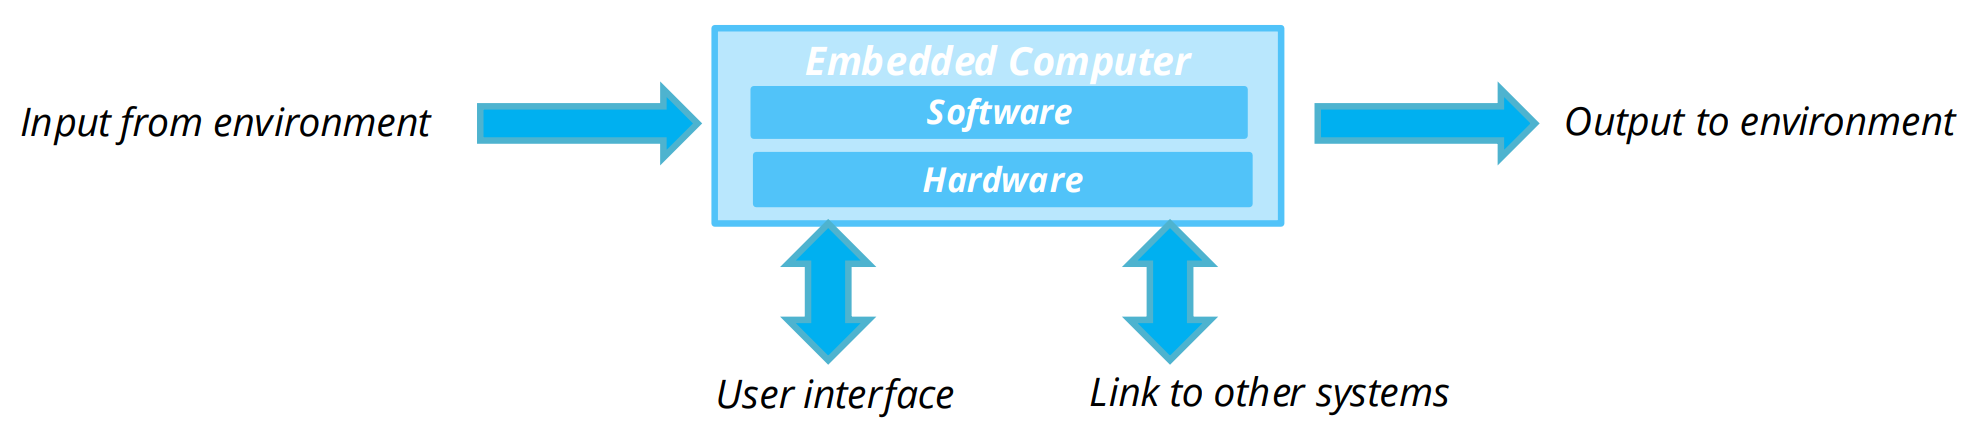
\includegraphics[width=0.8\linewidth]{img/img1.png}
    \caption{Embedded Computer}
\end{figure}

Another definition of embedded system: 

\begin{tcolorbox}[colback=blue!5!white, colframe=blue!50!white, arc=0mm, sharp corners]
\textbf{Application-specific} computer system often with \textbf{real-time computer constraints}.
Implemented using \textbf{MCUs}, MicroControllerUnit.
\end{tcolorbox}

\paragraph{}
Embedded systems are added to larger system for different reasons:

\begin{itemize}
    \item Lower cost;
    \item Lower performance;
    \item Energy efficiency;
    \item More Functions and Features.
\end{itemize}

\newpage
\subsection{Example of some Embedded Systems}

\paragraph{Bike Computer}

\begin{itemize}
    \item Functions: speed and distance measurements;
    \item Constraints: size, cost, power and energy, weight;
    \item Inputs: wheel rotation that indicate how fast we are;
    \item Output: Display the speed;
    \item Use Low-Performance Microcontroller: 8-bit, 10 MIPS.
\end{itemize}

We can see that all the constraint change the design, software and hardware integration.

\paragraph{Automotive Embedded System}

Nowadays, cars are fully of microprocessors that detect different events that occur while driving or not:

\begin{itemize}
    \item 4-bit microcontroller checks seat belts;
    \item Microcontrollers run dashboard device;
    \item 16/32-bit microprocessor controls the engine...
\end{itemize}


\section{Microprocessor VS Microcontroller}

What is the difference between  \textbf{Microprocessor}, CPU, and\textbf{Microcontroller}, MCU?


Both have a \textbf{CPU core} to execute instructions.

\subsection{Microprocessor, CPU}

The \textbf{microprocessor (CPU) is a single core processor} that support at least the instruction of \textit{fetching}, \textit{decoding} and \textit{executing}. 

Normally it is used for a general purpose computer, it also \textbf{need memory and I/O}.

\paragraph{}

Nevertheless, this CPU uses the same logic to perform \textbf{different tasks}, so we can change the \textbf{program} within the memory to perform different algorithms, thus simplifying the design and the usability.


\begin{figure}[H]
    \centering
    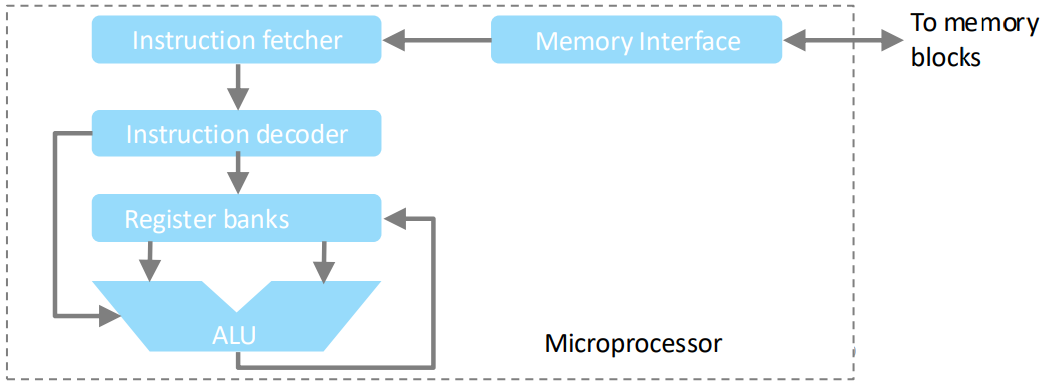
\includegraphics[width=0.8\linewidth]{img/img2.png}
    \caption{CPU schema}
\end{figure}

\paragraph{Alternative?} Field-Programmable Gate Arrays (also known as \textbf{FPGAs}), custom logic, etc. All of this things are a \textbf{dedicate hardware} that has a special purpose, indeed they are designed for a specific function. In general they use less power than CPU but they can not be used for other functions.

\paragraph{}

\textbf{Modern microprocessors} also offer features to control power consumption, via software we can reduce the consumption (sleep mode).

Microprocessor are used in combination with some custom logic for a well-defined functions, while the CPU and software is used for everything else.


\subsection{Microcontroller, MCU}

As written above, the MCU generally has a single-core processor, memory blocks, Digital and Analog I/Os and other basic pheripherals. It is typically used for a \textbf{basic control purposes}.

\begin{figure}[H]
    \centering
    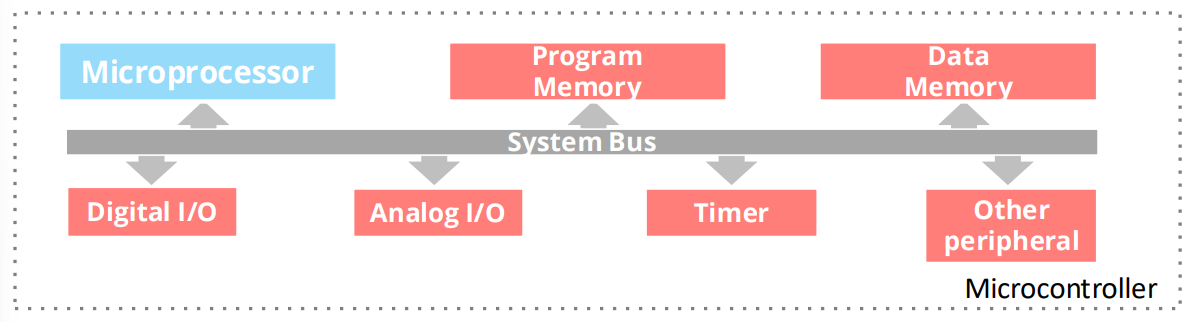
\includegraphics[width=0.8\linewidth]{img/img3.png}
    \caption{Microcontroller}
\end{figure}

\subsection{How to chose between CPUs and MCUs?}

In most embedded system, MCUs are chosen to be the best solution because they offers:

\begin{itemize}
    \item Low development and manufacturing cost;
    \item Easy porting and updating;
    \item Light footprint;
    \item Relatively low power consumption;
    \item Good performance for low-end products.
\end{itemize}

\begin{figure}[H]
    \centering
    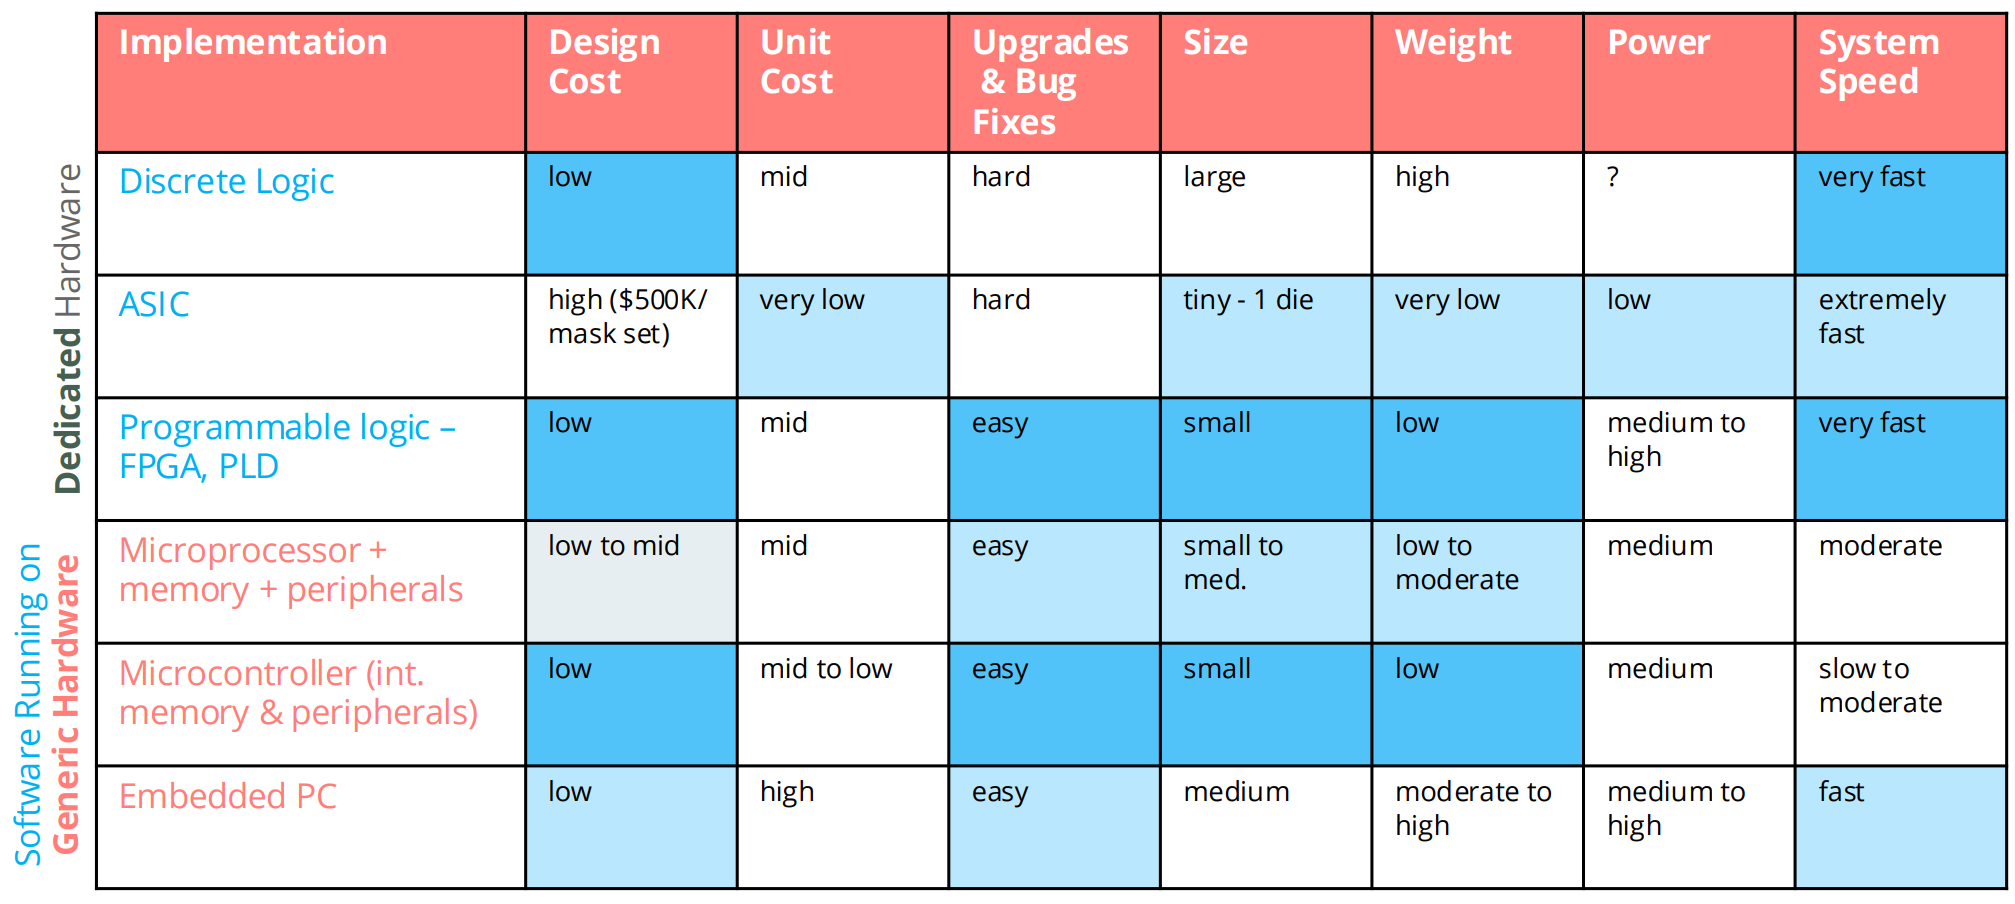
\includegraphics[width=1\linewidth]{img/img4.png}
    \caption{Options for Building Embedded Systems}
\end{figure}

Unless there's a very specific reason, such as some constraints, the best choice for embedded systems is
software running on generic hardware.


\subsection{Basic functionality of an Embedded System}

\begin{itemize}
    \item[] \textbf{Monitoring Applications: } monitor a process and adjust an output to maintain desired set point, e.g. temperature, speed...
    \item[] \textbf{Sequencing: } step through different stages, called states, based on environment and system;
    \item[] \textbf{Digital signal processing: } remove noise, select desired signal features;
    \item[]  \textbf{IoT applications: } exchange information reliably and quickly using near-by communications and networks.
\end{itemize}

\section{Challenges in Embedded System Design}

There are lots of challenges when we use the embedded system some could be: how much hardware do we need? How faster the CPU is? How do we meet our deadlines? faster HW or cleverer SW? How minimise power consumption? Turn off unnecessary logic or reduce memory accesses? How de we design for upgradeability? Is it secure?

\paragraph{}

\textbf{Testing on embedded system is complex: }we can not separate the testing of an embedded computer from the machine in witch it is embedded.
\paragraph{}
\textbf{Limited observability and controllability: }it is difficult to see how it happen, there is none screen and keyboards, we need to watch the electrical signal values.
\paragraph{}
\textbf{restricted development environments: }much more limited than those available for PCs.

\section{Attributes of Embedded Systems}

\subsubsection{Interfacing with the environment}

Analog signals from sensors, typically using a voltage value that rappresents a physical value.

\subsubsection{Concurrent and reactive behaviors: real-time constraints on responses}
Embedded systems are not single-threaded: a lot of things can happen simultaneously as they respond to
sequences and combinations of events in a timely manner.
Embedded systems typically must perform multiple separate activities concurrently, especially when
having several sensors.

\subsubsection{Fault handling}
Operate independently for long periods and handle likely faults \textbf{without crashing}


\subsubsection{Diagnostics}

Embedded systems should help developers determine problems quickly.


\subsection{Example Analog Sensor - Depth Gauge}

We want calculate how deep and underwater object is: 


\begin{itemize}
    \item[-] A sensor detects pressure and generate a proportional output voltage \textbf{Vsensor}
    \item[-] Hence an Analog to Digital converter calculate and transform the voltage into a digit 
\end{itemize}

\begin{lstlisting}[language=c++]
// Your Software
ADC_Code = adc_read();
V_sensor = ADC_code * V_ref / ADC_MASK;
Pressure_kPa = 250 * (V_sensor / V_supply + 0.04);
Depth_ft =33 * (Pressure_kPa - Atmos_Press_kPa) / 101.3;
//Actual relationship between depth and pressure
\end{lstlisting}


  \begin{minipage}{\linewidth}
      \centering
      \begin{minipage}{0.45\linewidth}
          \begin{figure}[H]
                \centering
                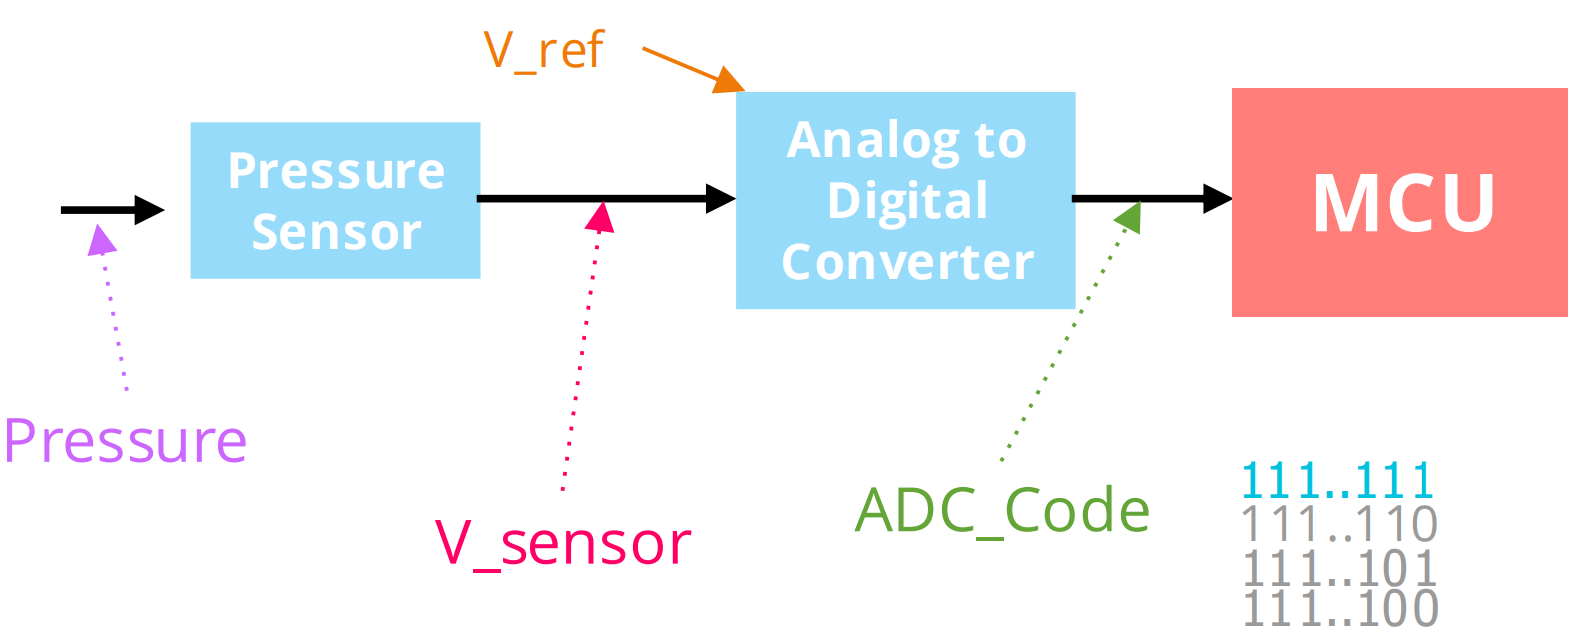
\includegraphics[width=1\linewidth]{img/img5.png}
          \end{figure}
      \end{minipage}
      \hspace{0.05\linewidth}
      \begin{minipage}{0.45\linewidth}
          \begin{figure}[H]
                \centering
                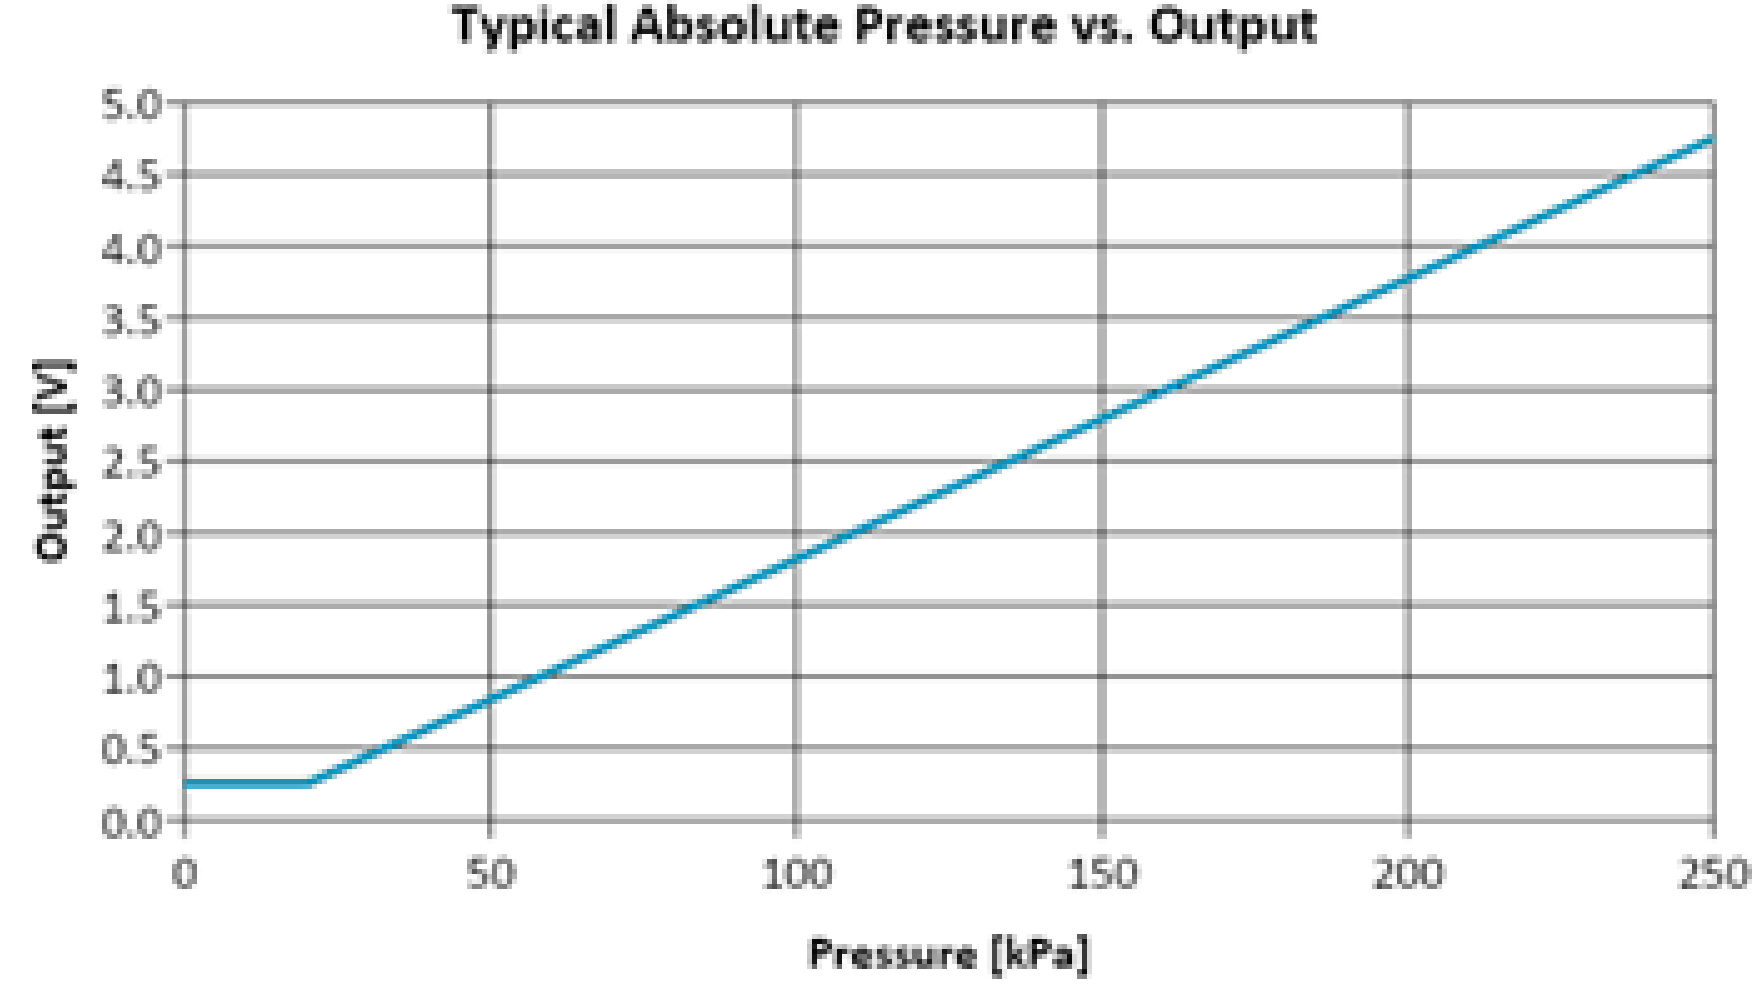
\includegraphics[width=1\linewidth]{img/image5.png}
          \end{figure}
      \end{minipage}
  \end{minipage}

\section{MCU Hardware \& Software for Concurrency}

In a microcontroller (MCU) several things happen \textbf{concurrently} while the CPU is executing instructions. 

Specialized hardware peripherals add dedicated \textbf{concurrent processing}, like analog interfacing, timers,
and detecting external signal events. Peripherals use interrupts to notify the CPU of events.

Embedded systems rely on both MCU hardware peripherals and software to get everything done concurrently on time


  \begin{minipage}{\linewidth}
      \centering
      \begin{minipage}{0.25\linewidth}
          \begin{figure}[H]
                \centering
                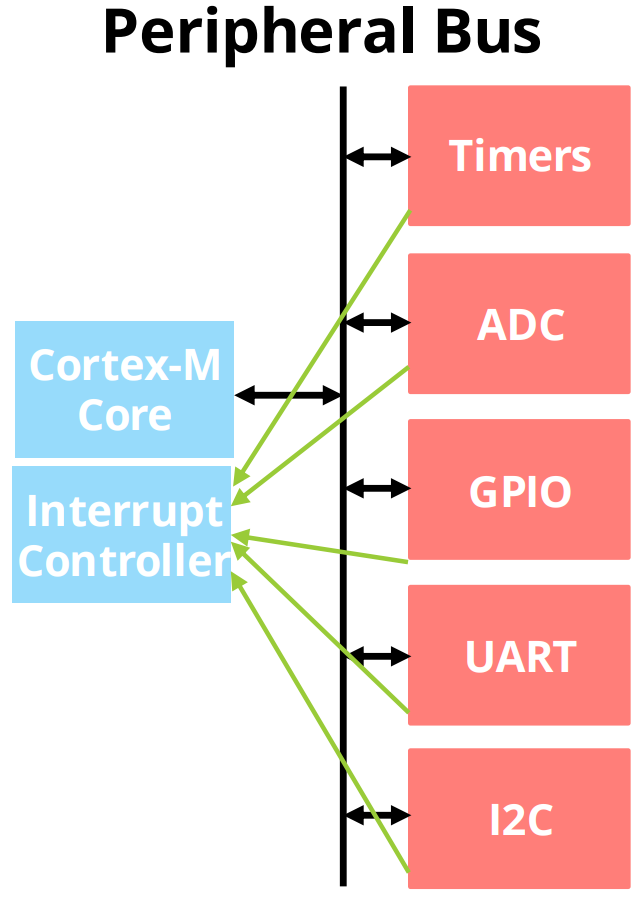
\includegraphics[width=1\linewidth]{img/image6.png}
          \end{figure}
      \end{minipage}
      \hspace{0.05\linewidth}
      \begin{minipage}{0.65\linewidth}
          \begin{figure}[H]
                \centering
                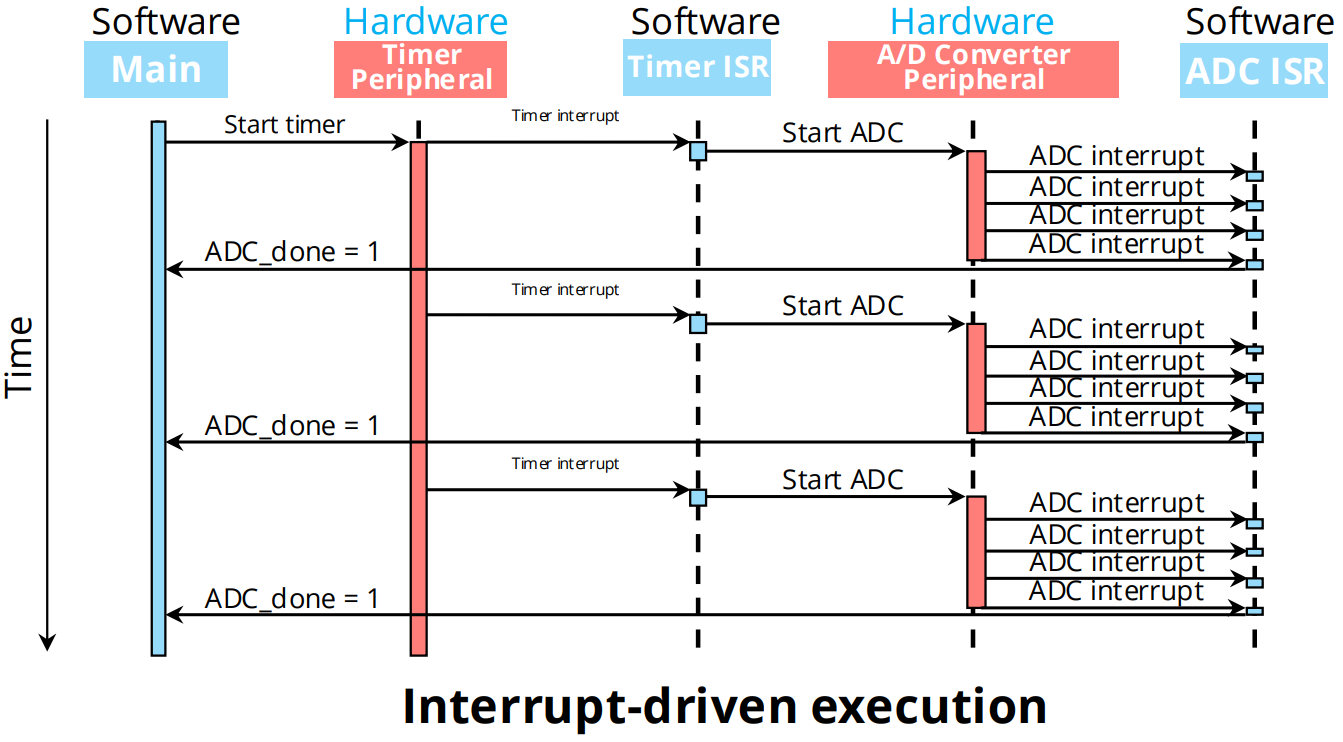
\includegraphics[width=1\linewidth]{img/image7.png}
          \end{figure}
      \end{minipage}
  \end{minipage}


\subsection{Embedded Software}

Programmed in C rather than Java (smaller and faster code, so less expensive MCU). Some performance-critical code may be in \textbf{assembly language}.

Typically, no OS, but instead a simple scheduler (or even just interrupts + main
code (foreground/background system). If OS is used, likely to be a lean \textbf{RTOS}


\subsection{Hardware and Software Co-design Model}

Commonly both the hardware and the software for embedded system are \textbf{developed in parallel}, this allow to optimize the overall
product's design, functionality and manufacturing/development cost.

Push things to the software layer if functionality can be achieved in software, this reduce  the  overall hardware \textbf{complexity} and cost.

\subsection{Functional vs. Non-functional Requirements}

Embedded systems have \textbf{MANY non-functional requirements} (how the system should perform). Timing
correctness is way more critical in embedded systems, especially in medical, transportation and
military systems.

Non-functional requirements can be: the time required to compute an output, the system's size, weight,
portability, power consumption, battery capacity, reliability and so on.


\paragraph{}
\textbf{Functional requirements are user-centric}, tangible and observable, and specify what the system must do.

\newpage
\section{Internet of Things (IoT)}
An Internet-of-Things system is a networked embedded
computing system. An IoT system is addressable
via a network.

Some examples are smart buildings and home appliances, wearable devices, medical devices.

\paragraph{}
Networking is a \textbf{critical component} of an IoT system

\subsection{Why IoT?}
\begin{itemize}
    \item[] Items can have more functionality and become more intelligent
    \item[] Items can be managed more easily
    \item[] More information becomes available
\end{itemize}


\subsection{Cyber-physical Systems}

Combines physical devices with computers that control the device. The embedded computer is the cyber part that replaces mechanical controllers:

\begin{itemize}
    \item more accurate and more sophisticated control
    \item monitors and controls the physical processes with feedback loops
\end{itemize}

\begin{figure}[H]
    \centering
    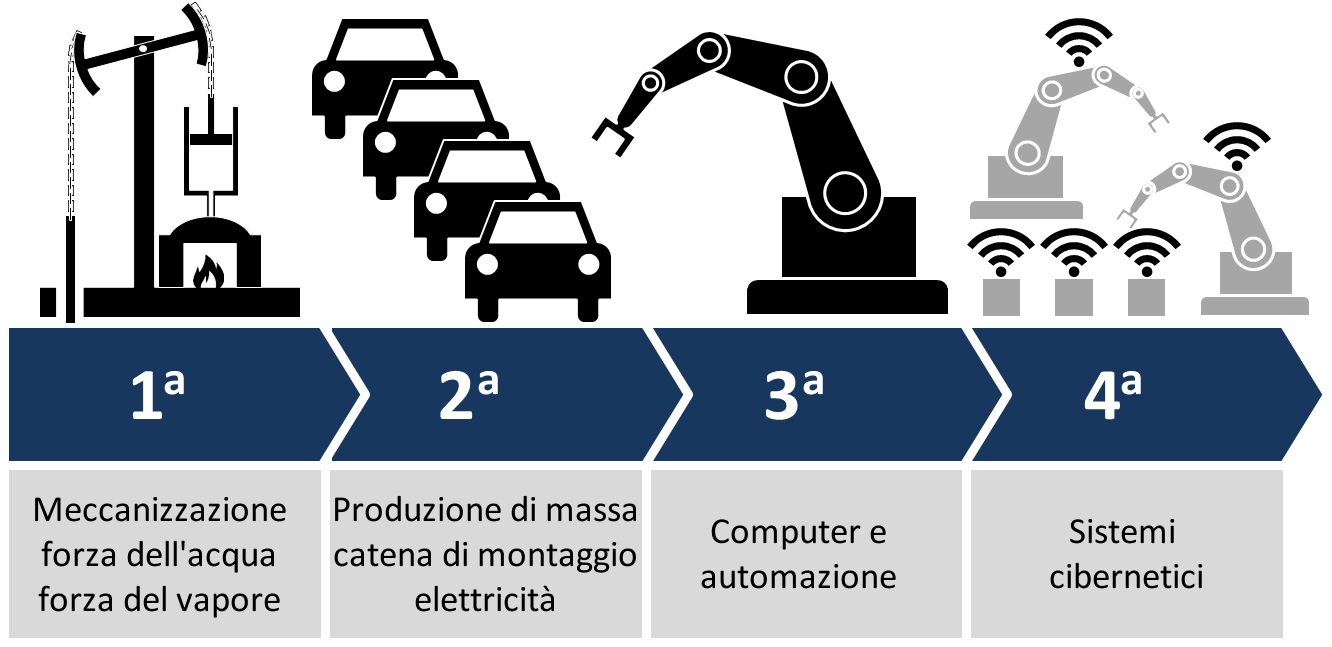
\includegraphics[width=0.5\linewidth]{img/Industry_4.0_ita.png}
\end{figure}

\section{Summary}

An embedded system is built for a specific application. It has complex hardware and software components.


Embedded systems pose many design challenges: Functional, output as a function of input, and non-functional requirements, Deadlines, power, cost.

In real-time systems, \textbf{timing correctness} is just as important as functional
or logical correctness
\chapter{Arm Cortex-M4 Processor and Its
Architecture}

\section{What is an ARM architecture?}

ARM stands for \textbf{Advanced RISC Machine}. It's a family of RISC-based processors, well-known for their
power efficiency and use in mobile devices (smartphones and tablets), designed and licensed by Arm to a
wide ecosystem of partners.

\section{RISC VS CISC}


\paragraph{Complex Instruction Set Computer (CISC):}
\paragraph{}
This processor offers a variety of instructions that perform very complex tasks like string searching and a
number of different instruction formats of varying lengths.

Examples of CISC processors are Intel processors.

\paragraph{Reduced Instruction Set Computer (RISC):}
\paragraph{}

This processor offers fewer and simpler instructions that can be efficiently executed in a pipelined manner,generally uses load/store instruction sets, operates only on register and cannot operate directly on
memory locations.


Overall, it's simplified hardware design and implementation which means that it will require less
power to use.


What is an ARM Cortex processor? What does it offer us? What are they main components?


\section{ARM Company}

Arm is the company that designs Arm-based processor cores. It does not manufacture them, but licenses
the designs to semiconductor partners which can add their own intellectual property (IP) on top of, which
then can fabricate and sell to customers.


\paragraph{}
Two types of licenses:

\begin{itemize}
    \item Microarchitectural License, which allows the vendor to use one of the various available Cortex licenses (RTL-level design of the processor).
    \item Architectural License, which allows the vendor to develop one's own microarchitecture based on ARM's ISA.
\end{itemize}

\section{How to Design an Arm-based SoC}

\begin{enumerate}
    \item Select a set of IP cores from Arm and/or other third-party IP vendors
    \item Integrate IP cores into a single-chip design
    \item Give design to semiconductor foundries for chip fabrication
\end{enumerate}

\begin{figure}[H]
    \centering
    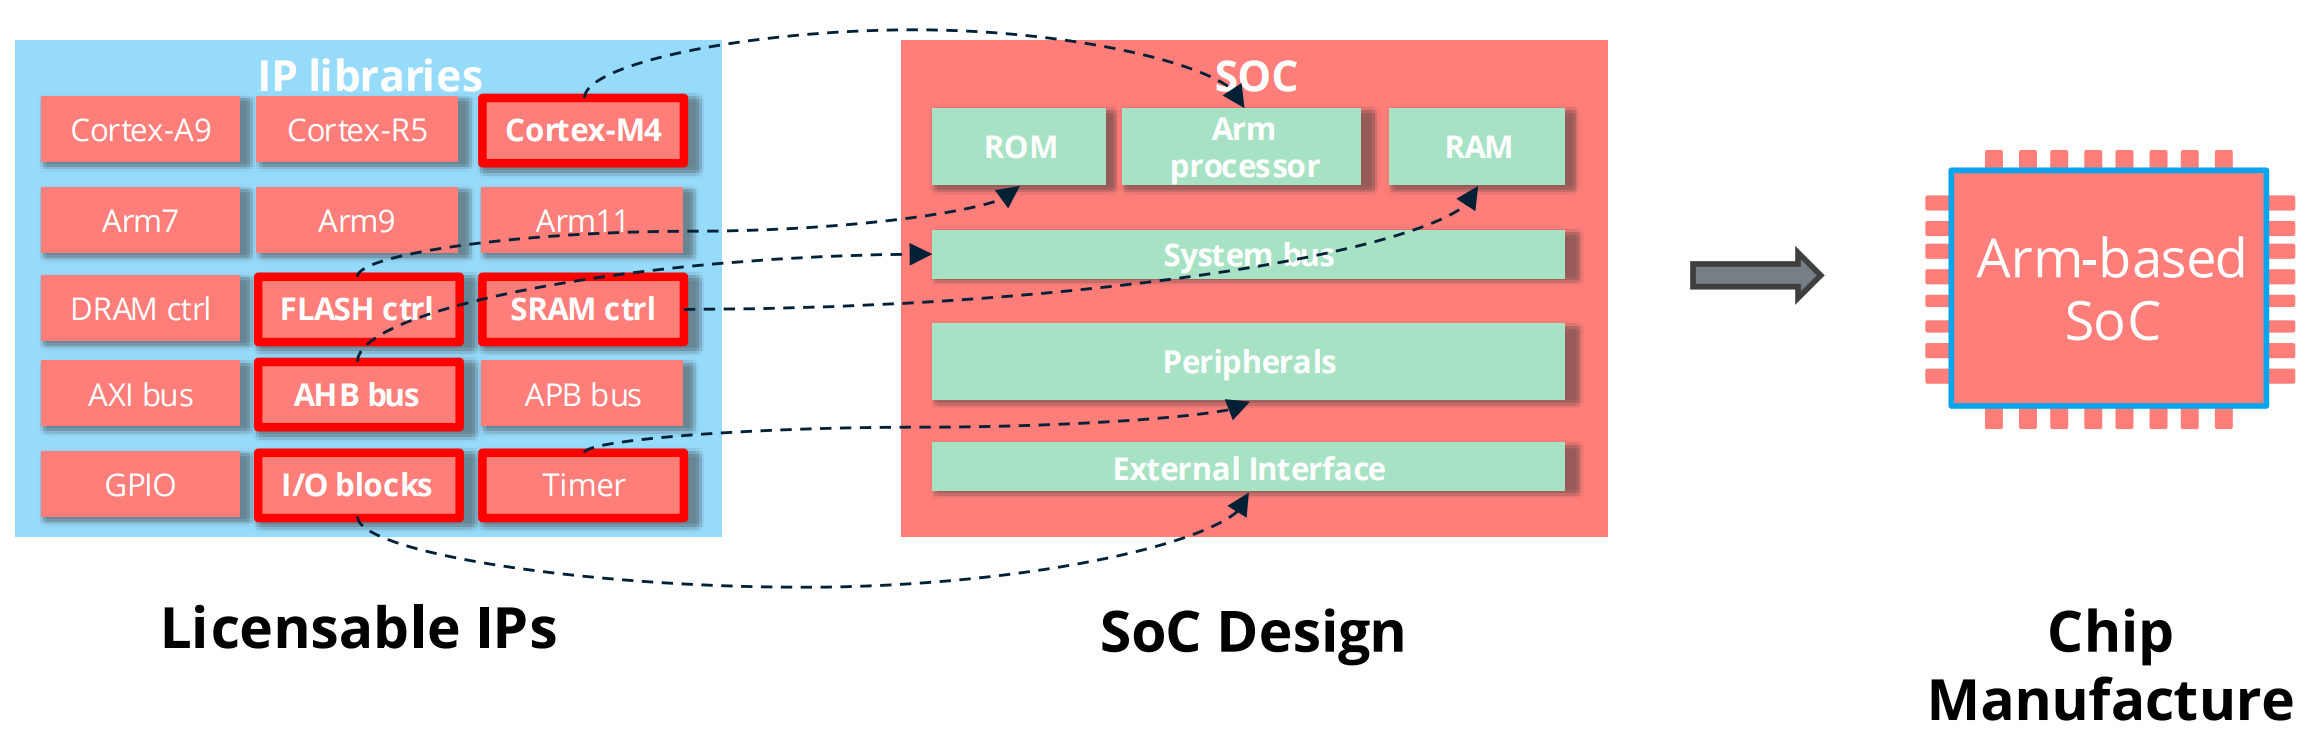
\includegraphics[width=1\linewidth]{img/image8.png}
\end{figure}

\section{Arm Processor Families}

\subsection*{Cortex-A series (Application)}
High performance processors capable of full operating system (OS) support. Applications include smartphones, digital TV, smart books.


\subsection*{Cortex-R series (Real-time)}
High performance and reliability for real-time applications. Applications include automotive braking systems, powertrains.


\subsection*{Cortex-M series (Microcontroller)}  

Cost sensitive solutions for deterministic microcontroller applications. Applications include microcontrollers, smart sensors.


\section{Arm Cortex-M Series}

The main features of a Cortex-M series processor are:

\begin{itemize}
    \item Energy efficiency
    \\ Low energy cost, which means longer battery life
    \item Smaller code
    \\ The code is smaller which means less memory is required, which means less power is consumed and hardware costs are lower
    \item Lower silicon costs
    \\ They occupy less physical space
    \item Ease of use and development
    \\ Faster software development and reuse (lots of tools)
    \item Targets several embedded applications
    \\ Like smart metering, human interface devices, automotive and industrial control systems, white goods (home appliances), consumer products and medical instrumentation
\end{itemize}

\section{Cortex-M series processors ranked}
The higher the number the better.

\subsection*{Cortex-M0 and Cortex M0+}

Cortex-M0 and Cortex-M0+ are for \textbf{applications requiring minimal cost, power and space}.
They're optimized for simple sensing and controlling.

\subsection*{Cortex-M3, Cortex-M4 and Cortex-M7}

These are \textbf{designed for data intensive applications requiring
higher performance}, like digital signal control applications. 

Cortex-M4 and Cortex-M7 integrate Digital Signal Processing (\textbf{DSP}) and \textbf{accelerated floating point processing capability} for fast and
power-efficient algorithm processing.

\section{Architectures and Implementations}

The architecture is the Instruction Set Architecture (ISA), which defines those characteristics and
instructions that must be true for all implementations.

Implementations are the actual hardware implementations of the architecture, which can have varying
clock speeds, different bus widths, different cache sizes and so on.


\section{Arm Architectures vs.Arm Processors}

\subsection*{Arm architecture}

The Arm architecture \textbf{describes the details of the instruction set}, the programmer's model, memory map.

\paragraph{}
Overtime, Arm architecture evolved to include architectural features that meet the growing demand for
new functionality (example: AI), integrated security features, high performance and the needs of new and
emerging markets.

\subsection*{Arm Processors}

The Arm processor is the implementation of the Arm architecture.

\begin{figure}[H]
    \centering
    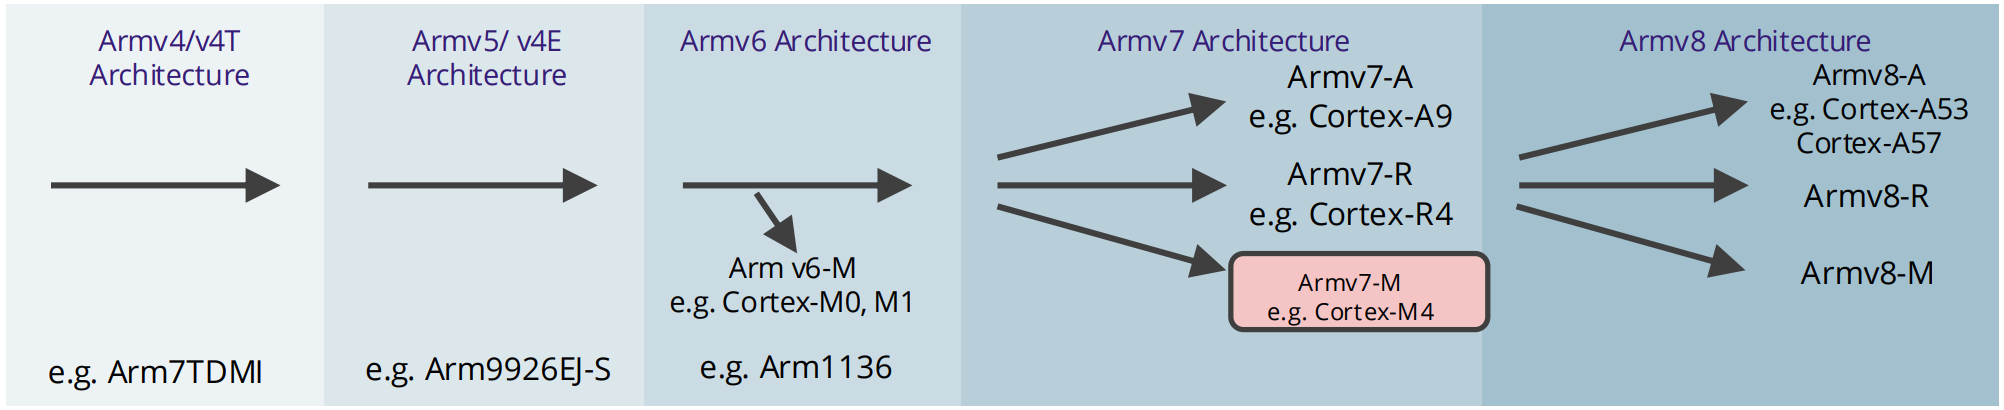
\includegraphics[width=1\linewidth]{img/image9.png}
\end{figure}

\begin{figure}[H]
    \centering
    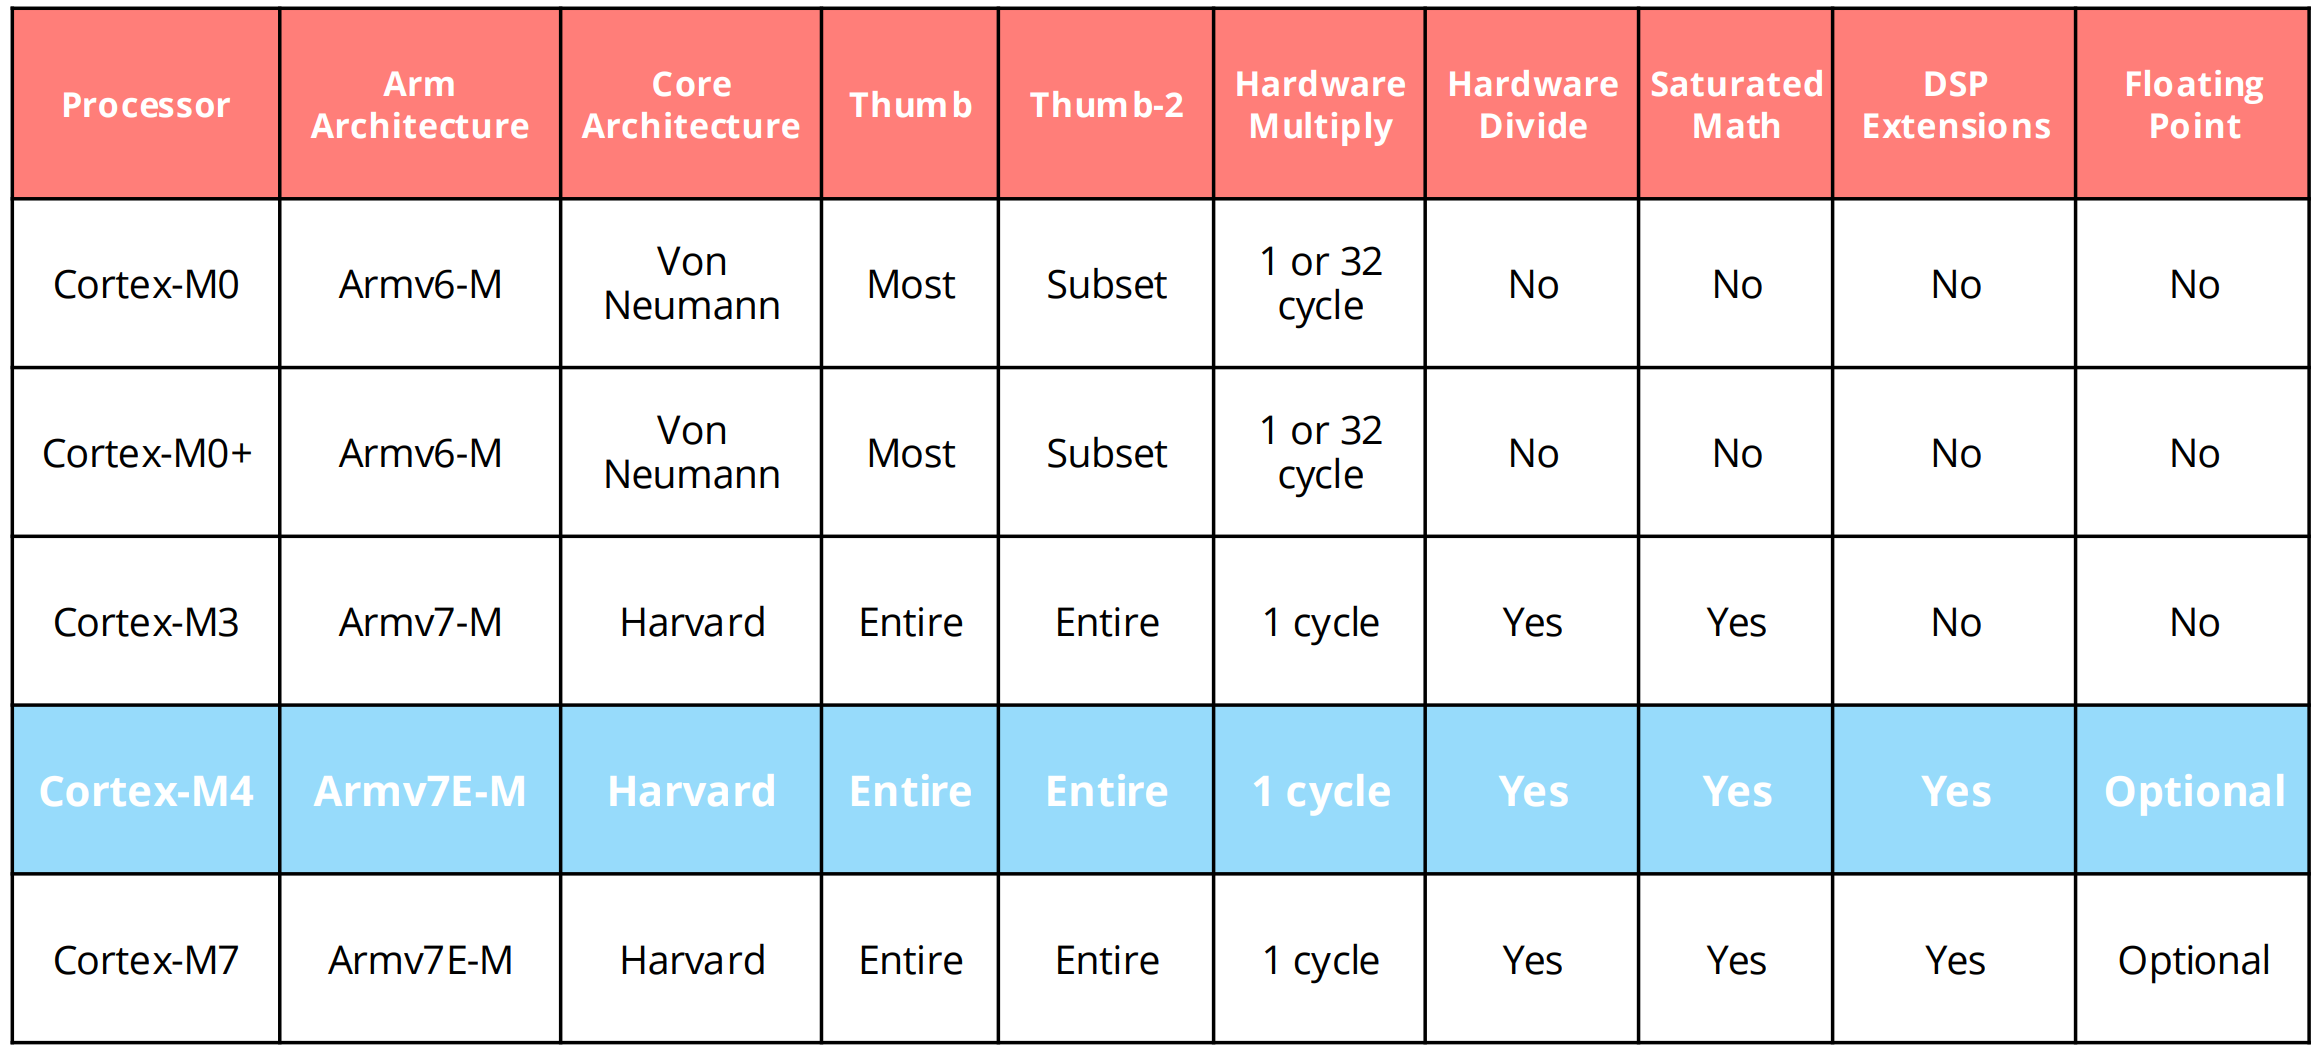
\includegraphics[width=1\linewidth]{img/image10.png}
\end{figure}


\section{Von Neumann Architecture }

The memory holds both data and instructions. CPU \textbf{fetches} instructions from memory, \textbf{decodes} them and
\textbf{executes} them.

The CPU register stores values used internally: program counter (PC), instruction register (IR), generalpurpose registers, etc.

\begin{figure}[H]
    \centering
    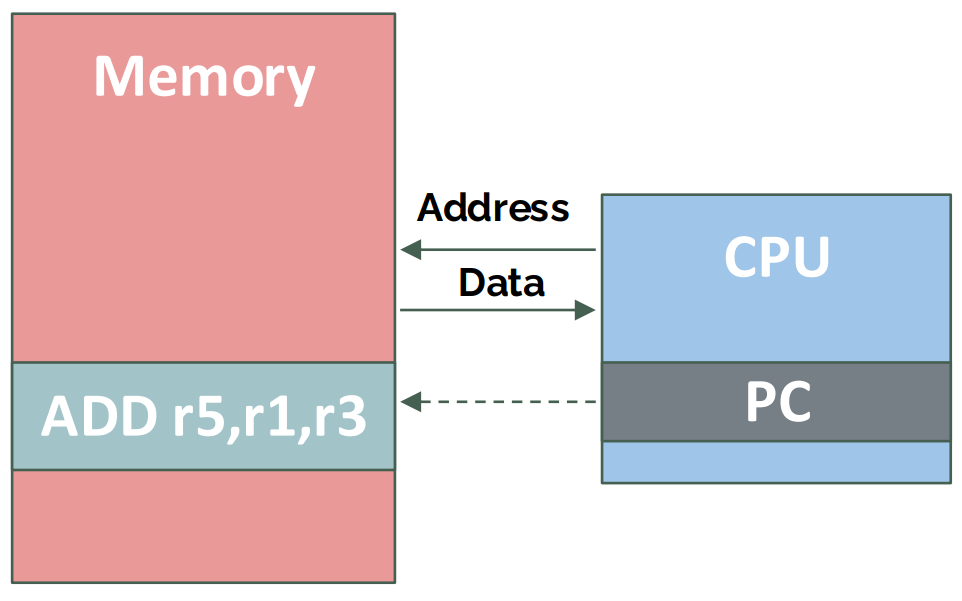
\includegraphics[width=0.4\linewidth]{img/image11.png}
\end{figure}


\section{Harvard Architecture}

There are two separate memories for data and program (instructions). Indeed the processor has two ports
for the two memories, so they don't compete for a single port, this \textbf{allows two simultaneous memory fetches}.

The program counter (PC) always points to program memory (not data memory) which means it cannot use self-modifying
code (secure).

\paragraph{}
Most DSPs are Harvard architectures. The separation of program and data memories provides \textbf{higher
performance}.


\begin{figure}[H]
    \centering
    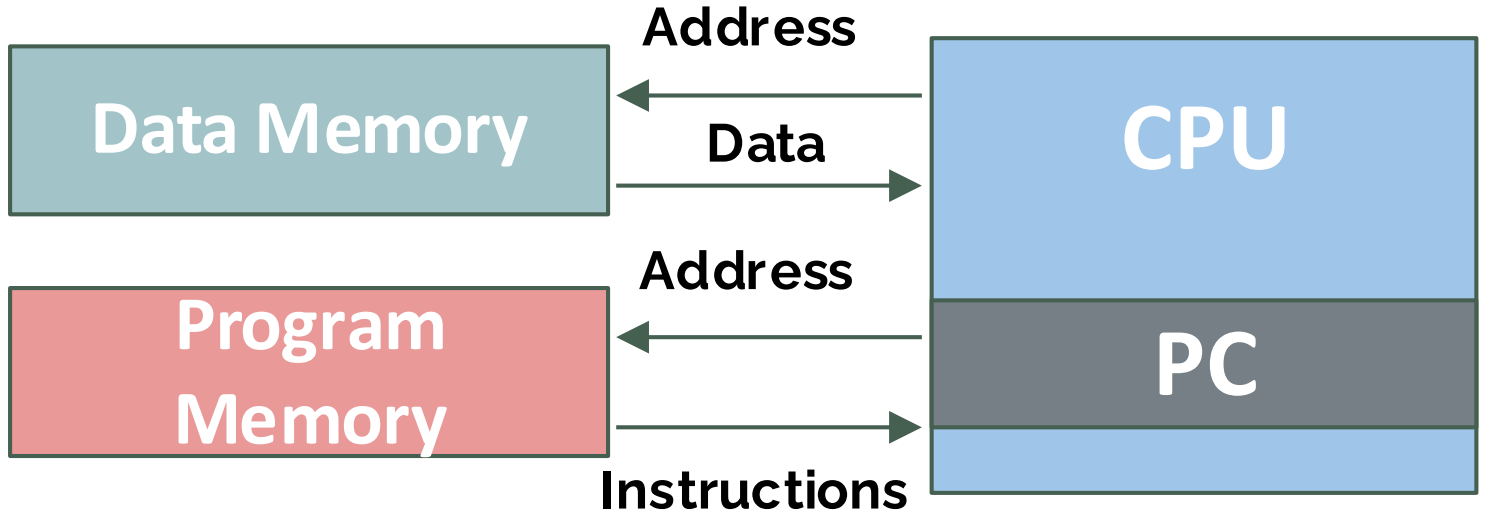
\includegraphics[width=0.5\linewidth]{img/image12.png}
\end{figure}

\section{Cortex-M4 Processor Overview}

The Cortex-M4 processor is designed with a large variety of highly efficient signal processing features
(example: single-cycle multiply accumulate instructions).

\paragraph{}
The \textbf{Multiply-Accumulate} (MAC) Instruction is an important and expensive operation mainly employed in
digital signal processing and video/graphics applications, machine learning included, that computes the
product of two numbers and adds that product to an accumulator.

\paragraph{}
It also features low power consumption, which means a longer battery life on the device that uses it, a
critical non-functional requirement in mobile products.

Furthermore it offers enhanced determinism: critical tasks and interrupt routines can be served quickly in
a known number of cycles. This is crucial for embedded system applications.

\subsection{Cortex-M4 Processor Features}

\textbf{32-bit} reduced instruction set computing (RISC) processor, \textbf{Harvard architecture}, so separate data bus and instruction bus and it has 3-stage + \textbf{branch speculation pipeline}.

\paragraph{}
It supports sleep modes: Features wake-up interrupts, with wait for interrupt (WFI) and wait for event (WFE) instructions.

Enhanced instructions Hardware divid, MAC, and so on.

\begin{figure}[H]
    \centering
    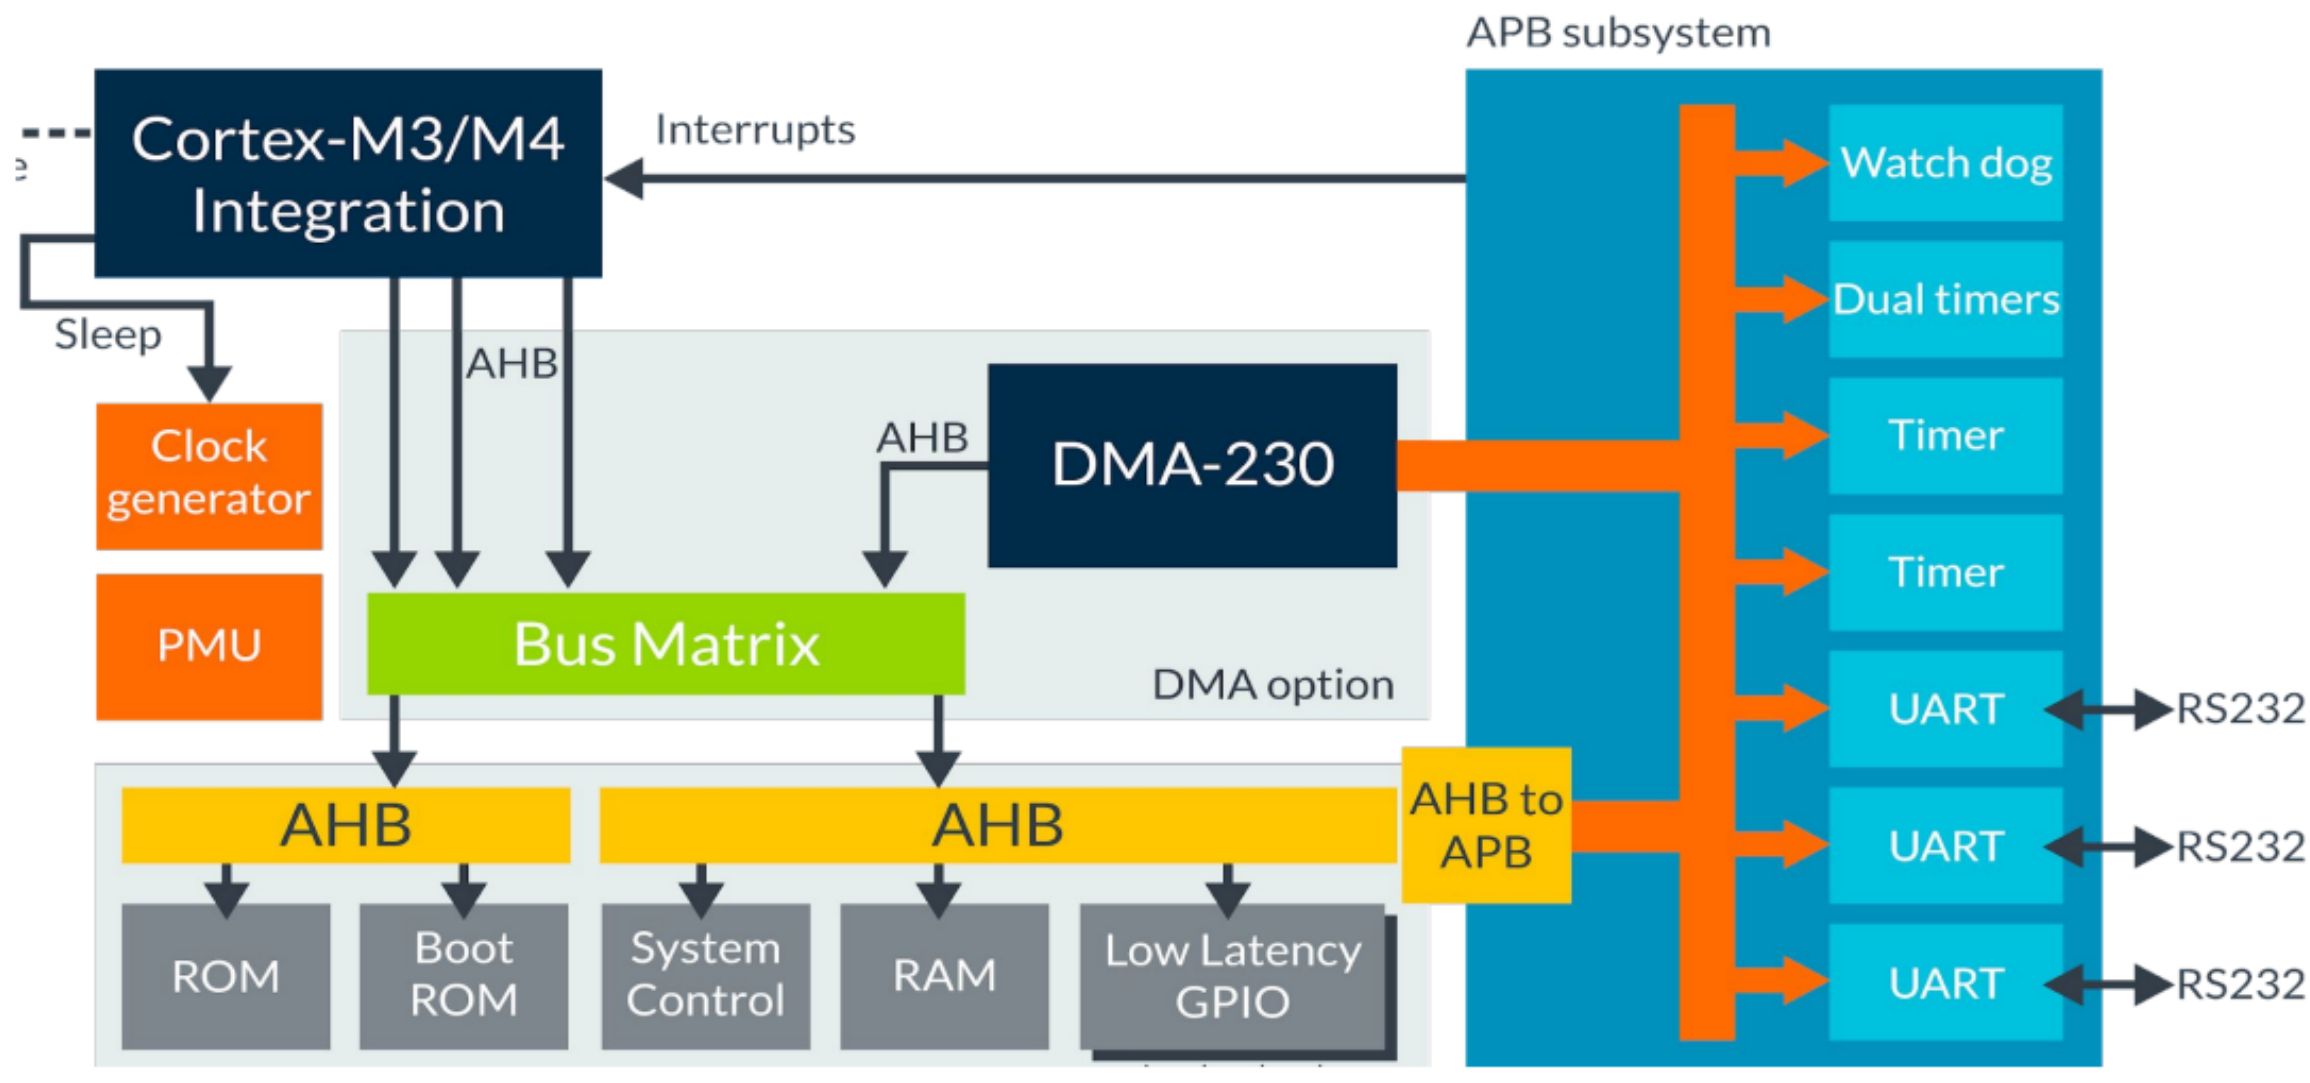
\includegraphics[width=1\linewidth]{img/image13.png}
    \caption{Arm M4-MCU Architecture}
\end{figure}

\subsection{Cortex-M4 Block Diagram}

\begin{figure}[H]
    \centering
    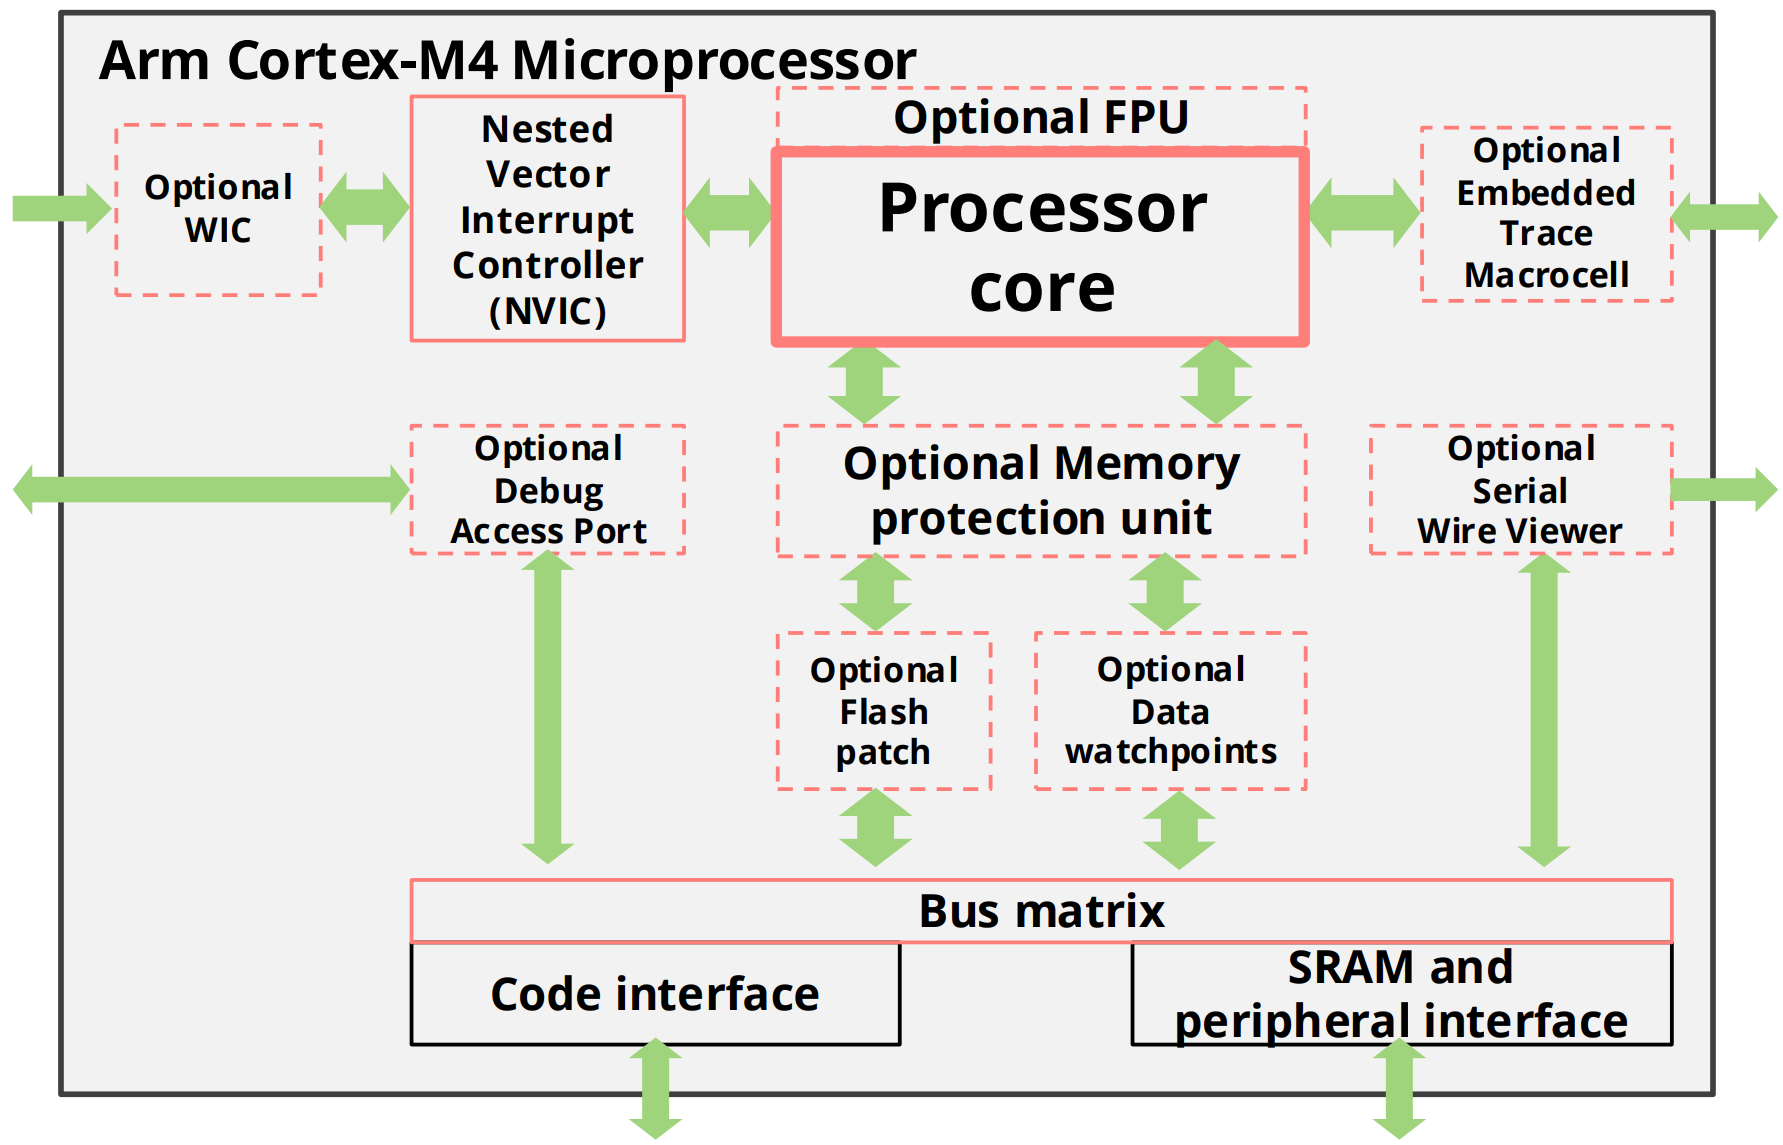
\includegraphics[width=0.8\linewidth]{img/image14.png}
\end{figure}

Here are the components as described:

\subsubsection{Processor core}

The processor core contains internal registers, the ALU, data path and some control logic.

It has a three-stage pipeline: fetch, decode, execution. Some instructions may take multiple cycles to
execute in which case the pipeline will be stalled. Also the pipeline speculatively prefetches instructions
from branch target addresses.

\begin{figure}[H]
    \centering
    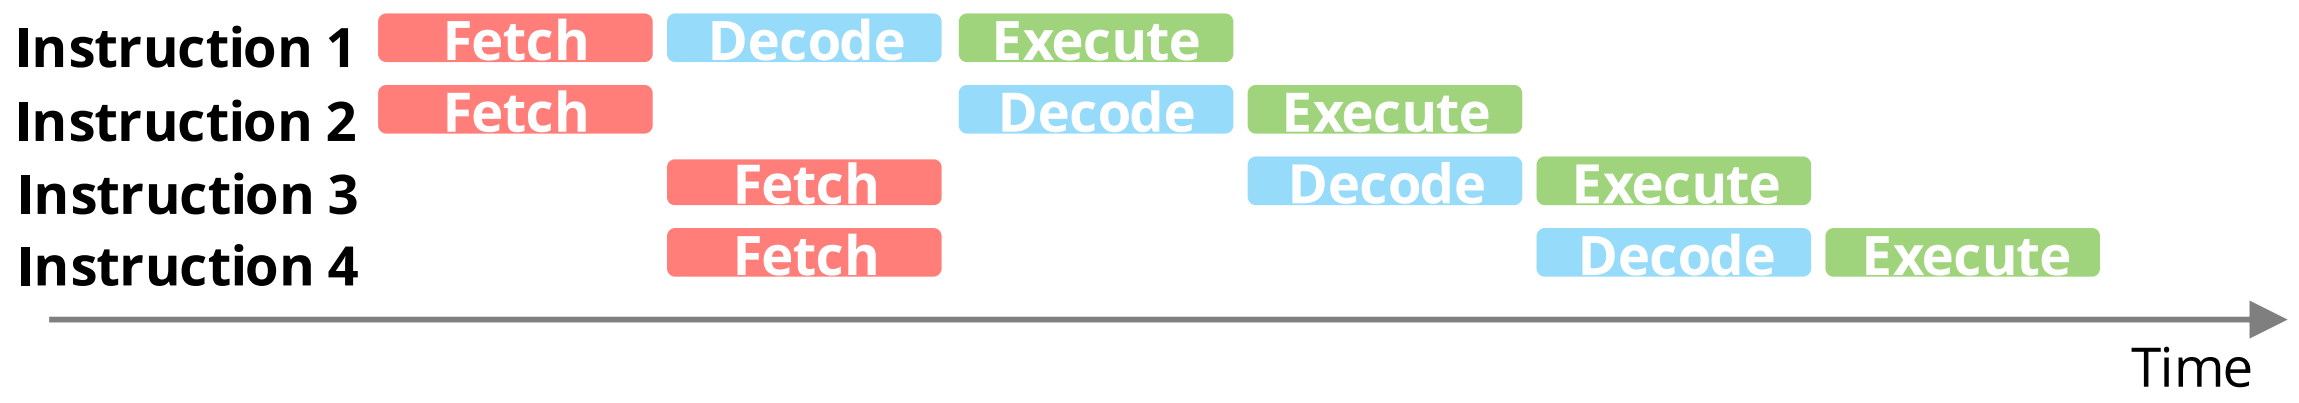
\includegraphics[width=0.8\linewidth]{img/image15.png}
\end{figure}

\subsubsection{Nested vectored interrupt controller (NVIC)}
It automatically handles nested interrupts, such as comparing priorities between interrupt requests and
the current priority level.

\subsubsection{Wake-up interrupt controller (WIC)}
For low-power applications, the microcontroller can enter sleep mode by shutting down most of the
components.

When an interrupt request is detected, the WIC can inform the power management unit to power up the
system.

\subsubsection{Memory protection unit (MPU)}

It is used to protect memory content. It makes some memory regions read-only and prevents user
applications from accessing each other.


\subsubsection{Debug subsystem - Embedded Trace Macrocell and Serial Wire Viewer}

It handles debug control, program breakpoints, and data watchpoints.


When a debug event occurs it can put the processor core in a halted state, so that developers can
analyse the status of the processor like register values and flags at that point.

\subsubsection{Bus matrix/Bus interconnect}

It provides data transfer management among hardware components and peripherals.

It also allows data transfer to take place on different buses simultaneously:

\begin{itemize}
    \item Advanced High-performance Bus (AHB)-Lite bus for high bandwidth peripherals
    \item Advanced Peripheral Bus (APB) interface. Low-power, meant for peripherals such as timers, interrupt controllers, UARTs, I/O
\end{itemize}

The bus matrix may include bus bridges (example: AHB-to-APB bus bridge) to connect different buses
into a network using a single global memory space.


\section{Programming Model}

The programming/programmer model is the set of registers available for use by programs.

The CPU has many other special purpose registers that are used for internal operations, which are
unavailable to programmers.


\subsection{Arm Cortex-M4 Processor Registers}

\begin{figure}[H]
    \centering
    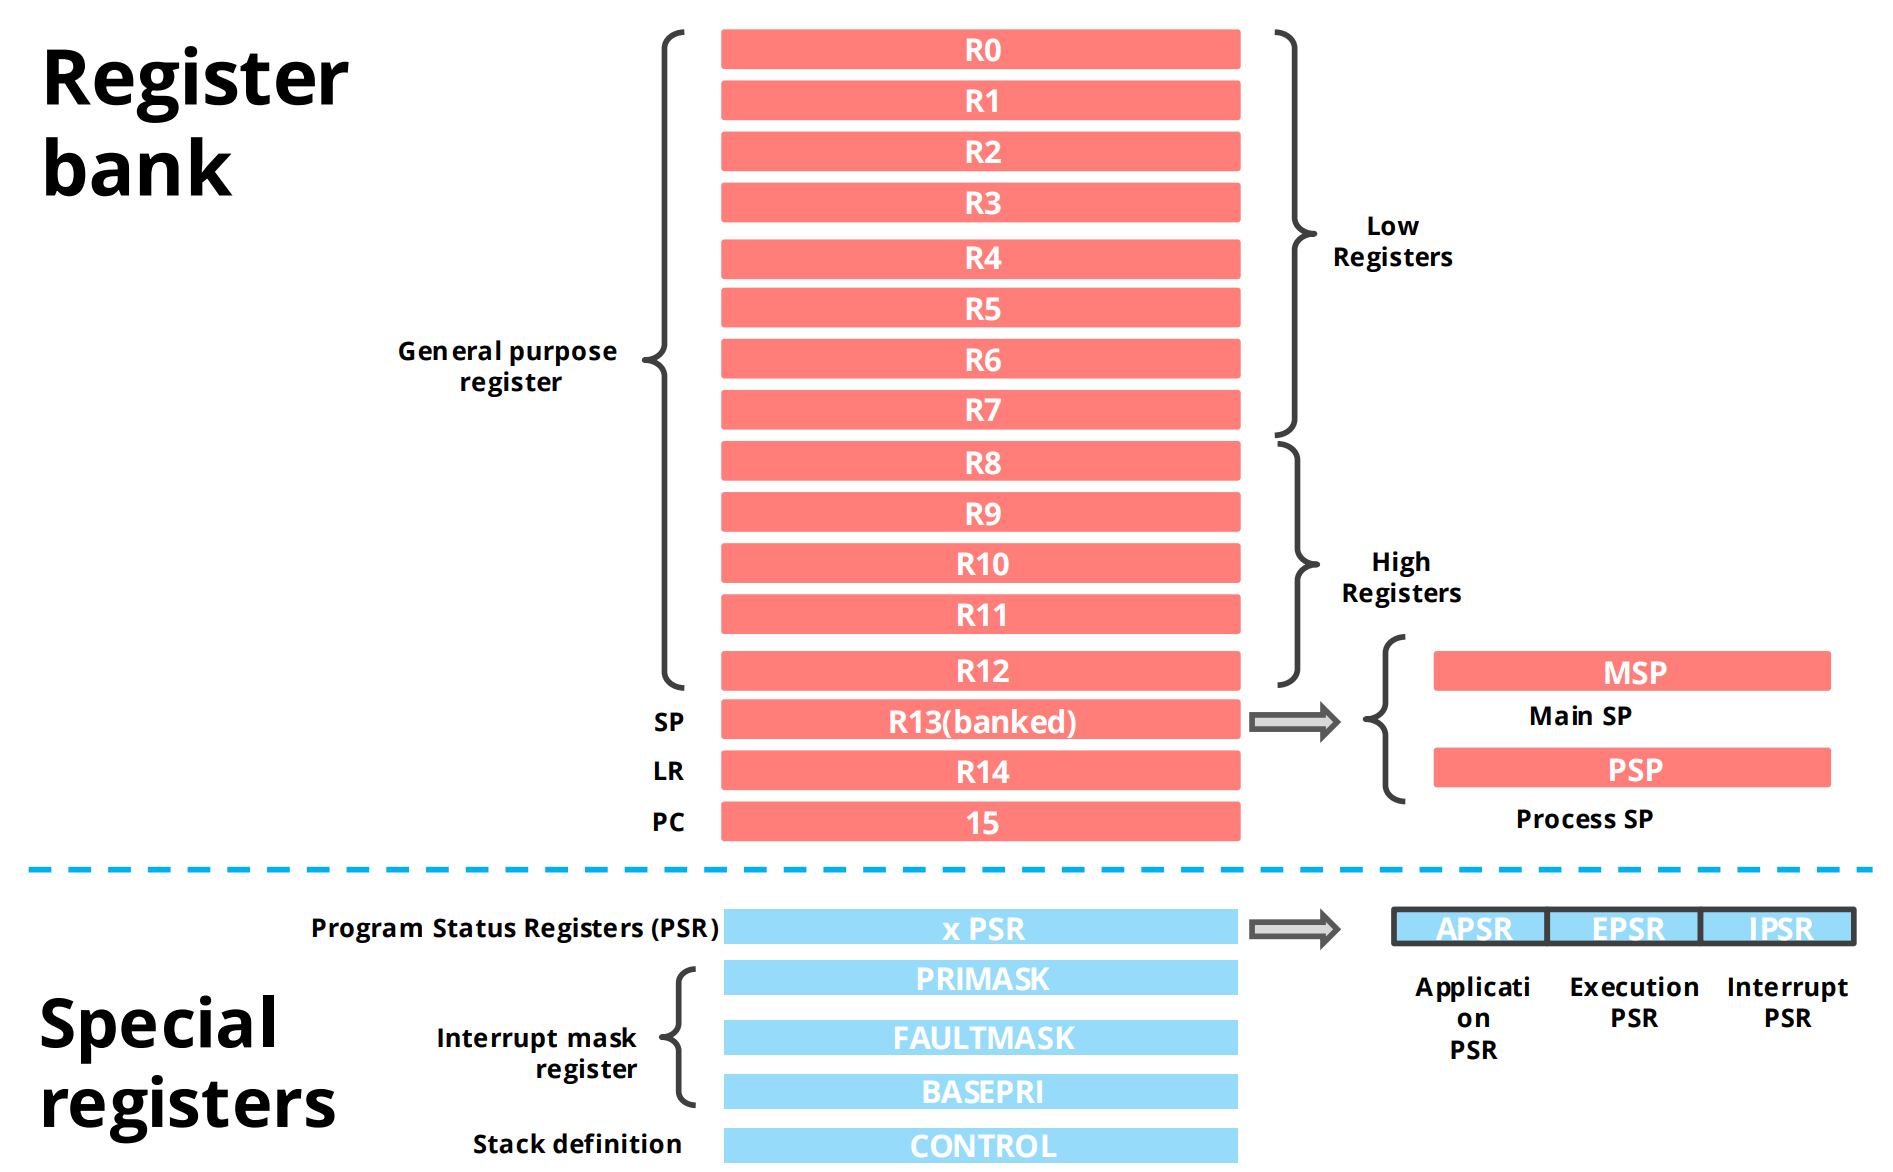
\includegraphics[width=0.8\linewidth]{img/image16.png}
\end{figure}


The processor registers store and process temporary data within the processor core quickly.


They follow a load-store architecture, in which to process memory data, they first have to be loaded from
memory to registers, processed inside the processor core using register data only, and then written back
to memory if needed.

\paragraph{}
The Cortex-M4's register bank is composed of 16 X 32-bit registers (R0-R12 are general-purpose, others
are the stack pointer (R13), the link register (R14) and the program counter (R15)).

\subsubsection{Stack Pointer}
The stack pointer (SP) records the current address of the stack and is used for saving context while
switching between tasks.

The Cortex-M4 has two SPs: the main SP, used in applications that require privileged access like the OS
kernel, and the process SP which is used in base-level application code.


\subsubsection{Program Counter}

The program counter (PC) records the address of the current instruction code and is automatically
incremented.

\begin{figure}[H]
    \centering
    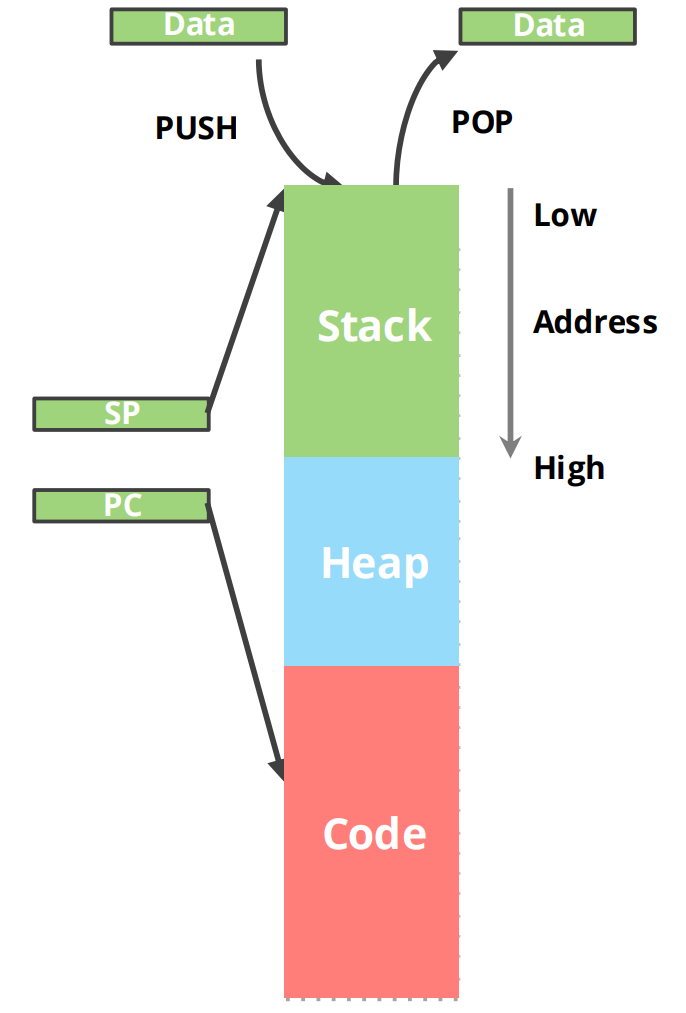
\includegraphics[width=0.25\linewidth]{img/image17.png}
\end{figure}

\subsubsection{Linik Register}
The link register (LR) stores the return address of a subroutine or function call. The PC will load the
value from the LR after a function is finished.

\begin{figure}[H]
    \centering
    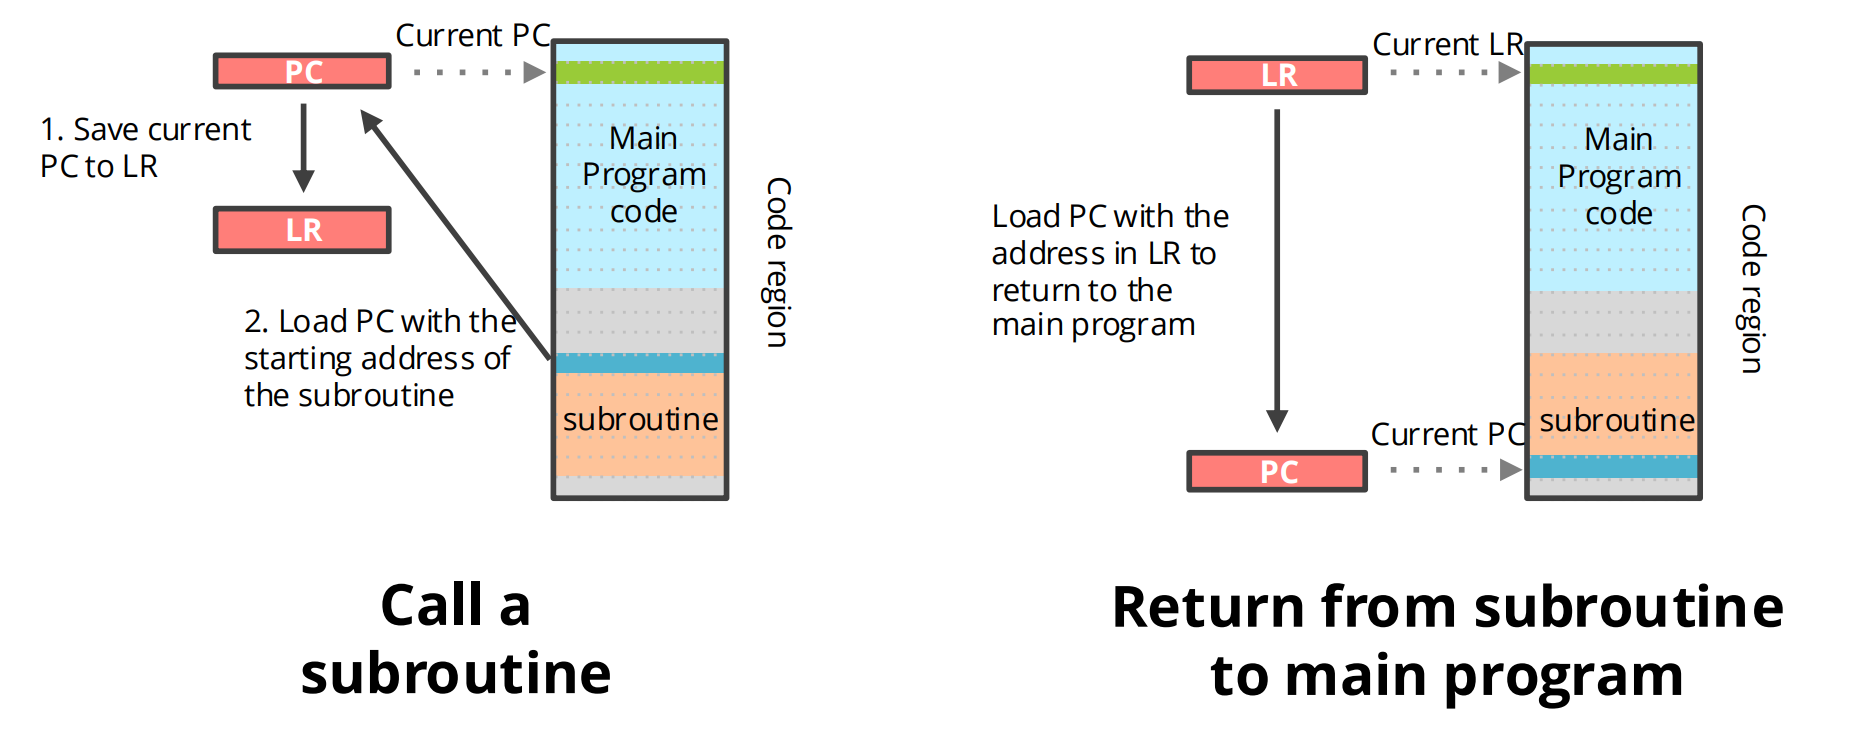
\includegraphics[width=0.85\linewidth]{img/image18.png}
\end{figure}

\subsection{Cortex-M4 Registers (Special Registers)}
Then there are special registers like the interrupt mask register used to enable/disable interrupts, the
program status registers (PSR) to understand what kind of exceptions, interruptions and results occurred.

\paragraph{}
The \textbf{xPSR}, \textbf{combined program status register}, provides information about program execution and
Arithmetic Logic Unit (ALU) flags. It combines the Application PSR, Interrupt PSR and Execution PSR.

\begin{figure}[H]
    \centering
    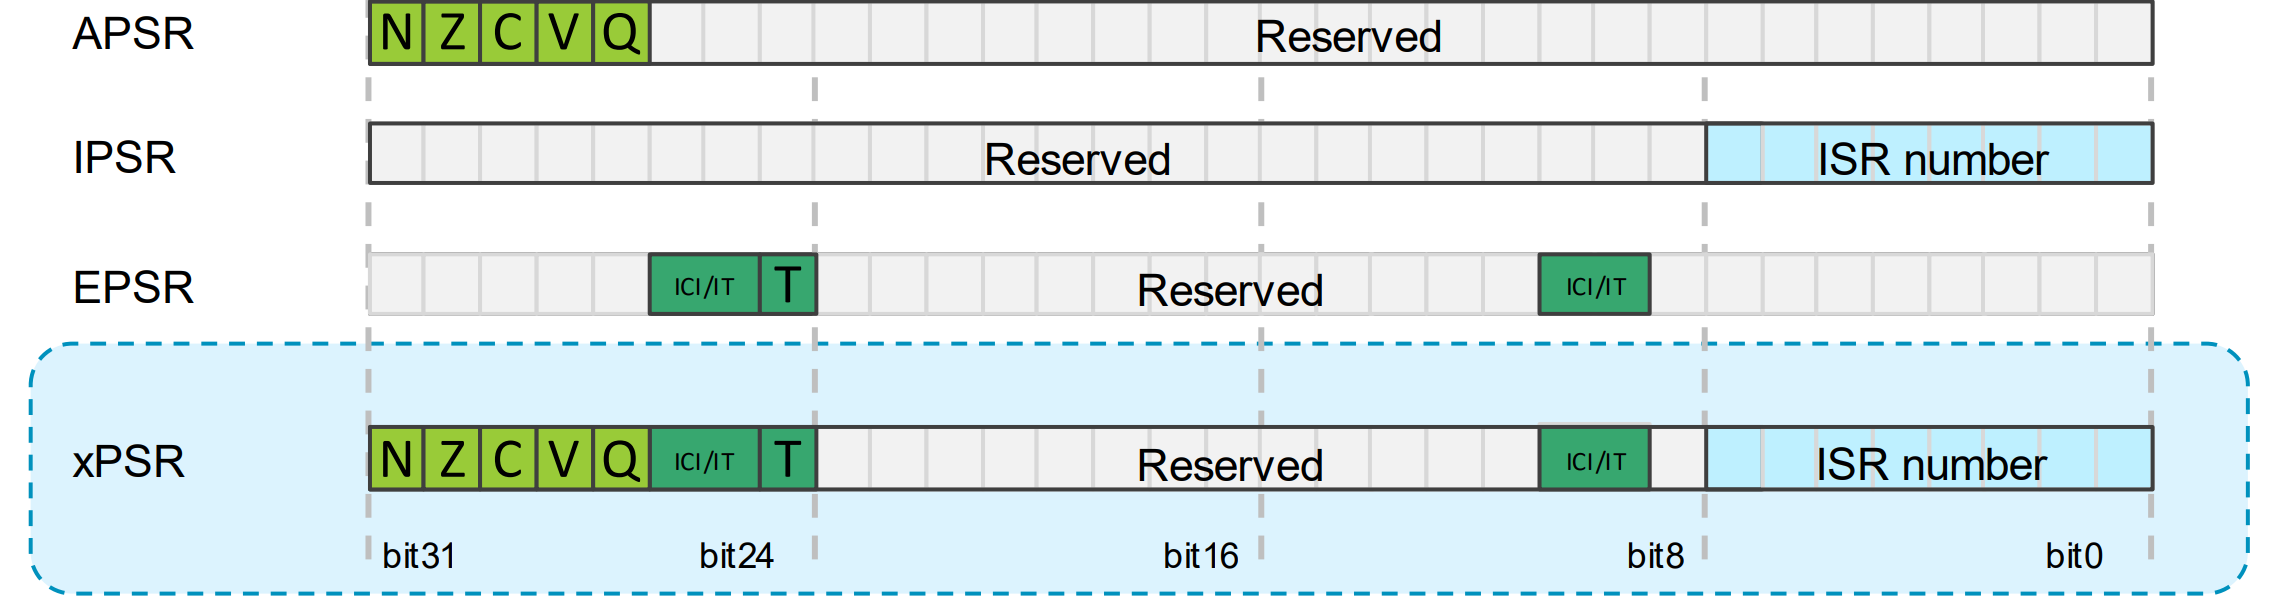
\includegraphics[width=1\linewidth]{img/image19.png}
\end{figure}

\paragraph{APSR - Application Program Status Register}

\begin{itemize}
    \item[-] N: negative flag
    \item[-] Z: zero flag
    \item[-] C: carry flag
    \item[-] V: overflow flag
    \item[-] Q: stick saturation flag
\end{itemize}


\section{Arm Cortex-M4 Memory Map}

The \textbf{memory map} describes the organization of the \textbf{processor’s address space}.

ARM memory is \textbf{byte-addressable} using \textbf{32-bit} addresses. The Cortex-M4 processor has \textbf{4GB of memory address space}.

The 4GB memory address space is architecturally defined with a number of regions, each one designed
for particular recommended use cases, making it easy for a software programmer to port between
different devices.

\paragraph{}
Memory map can also be flexibly defined by the user, apart from some fixed memory addresses such as
internal private peripheral bus.


\begin{figure}[H]
    \centering
    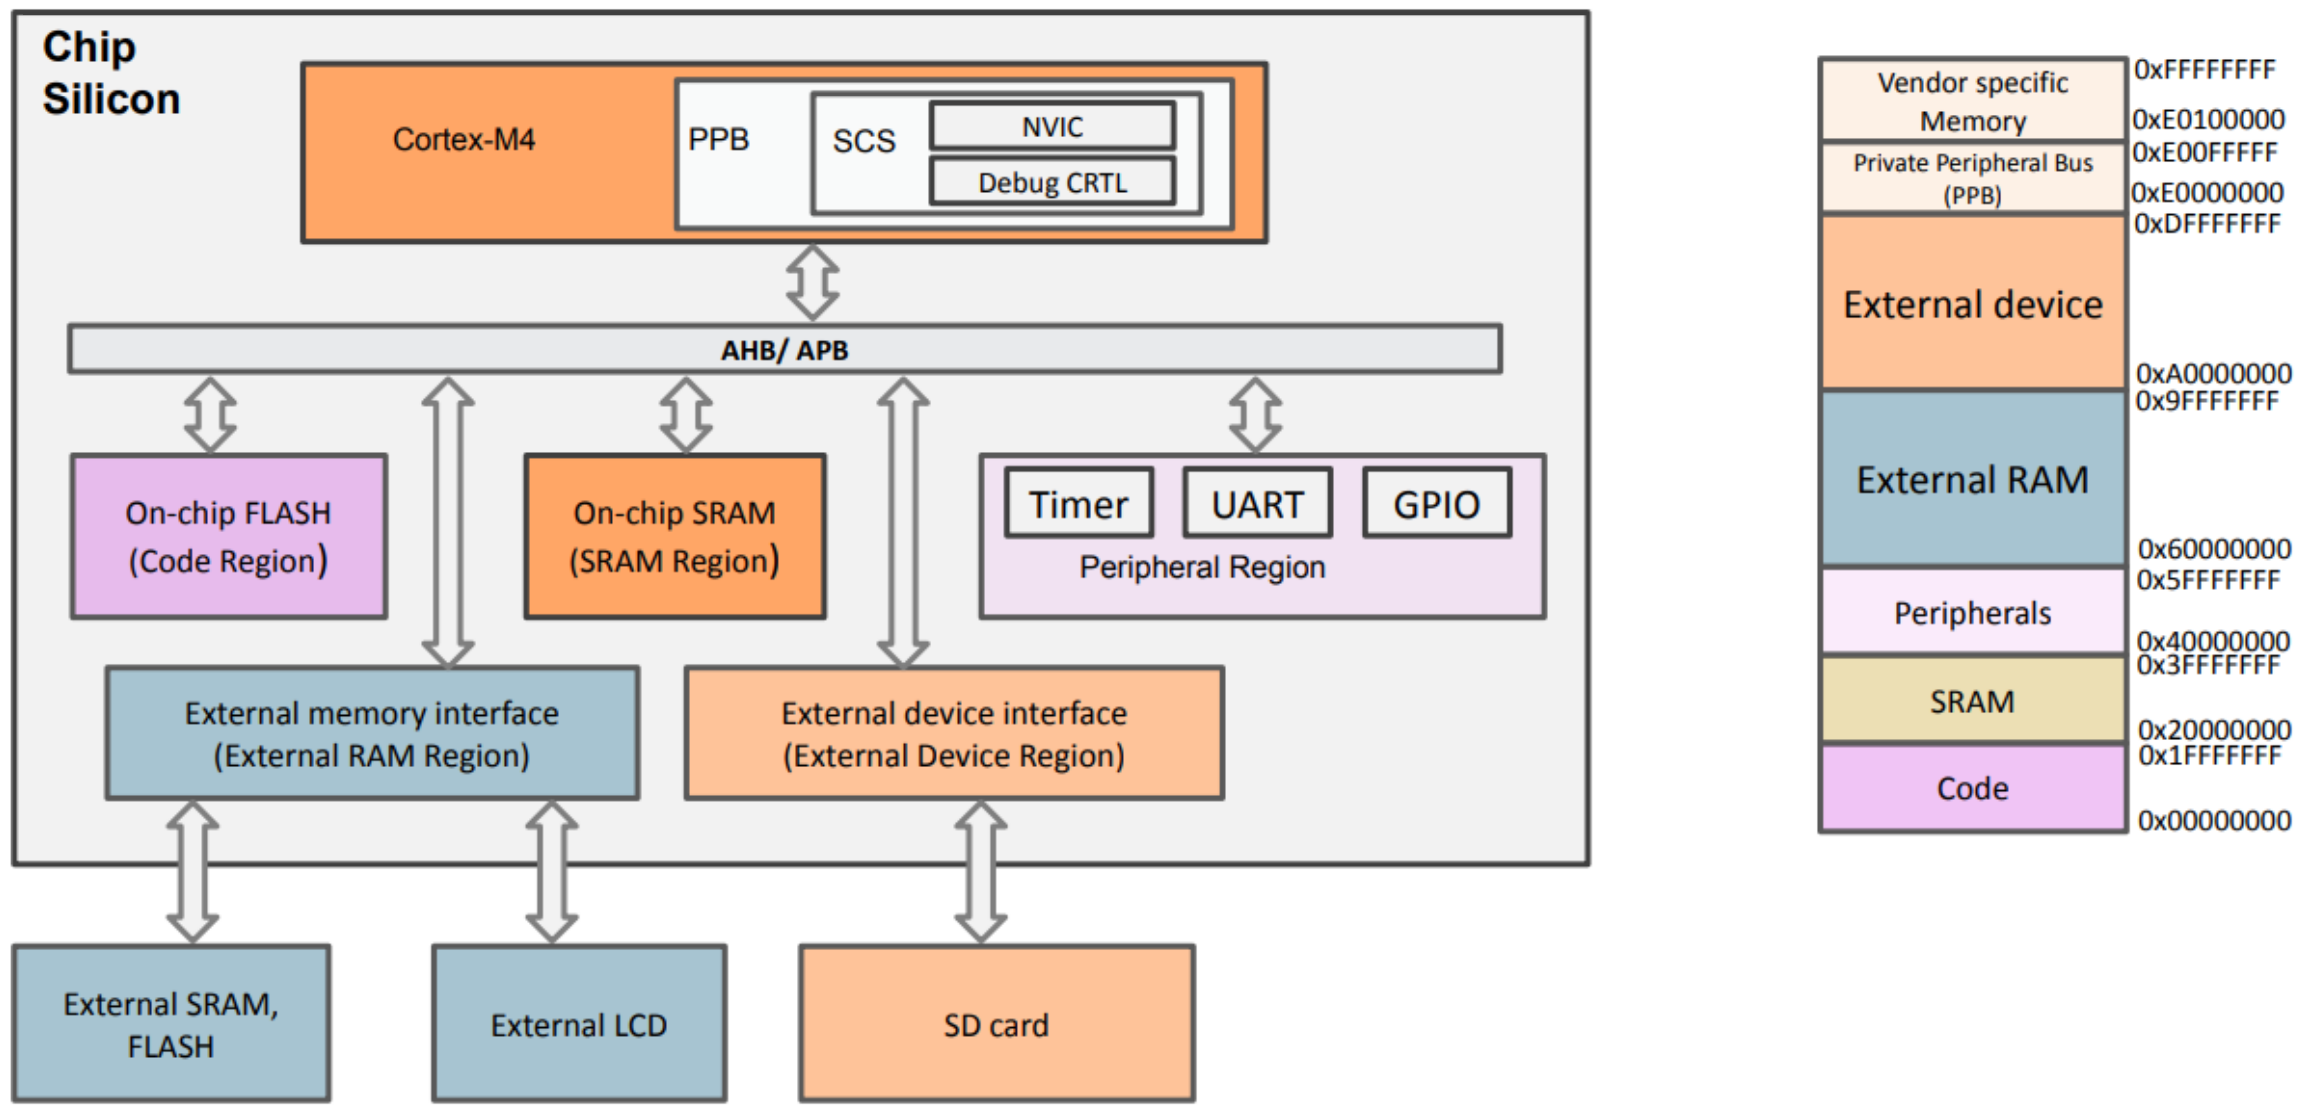
\includegraphics[width=1\linewidth]{img/image20.png}
\end{figure}


\begin{figure}[H]
    \centering
    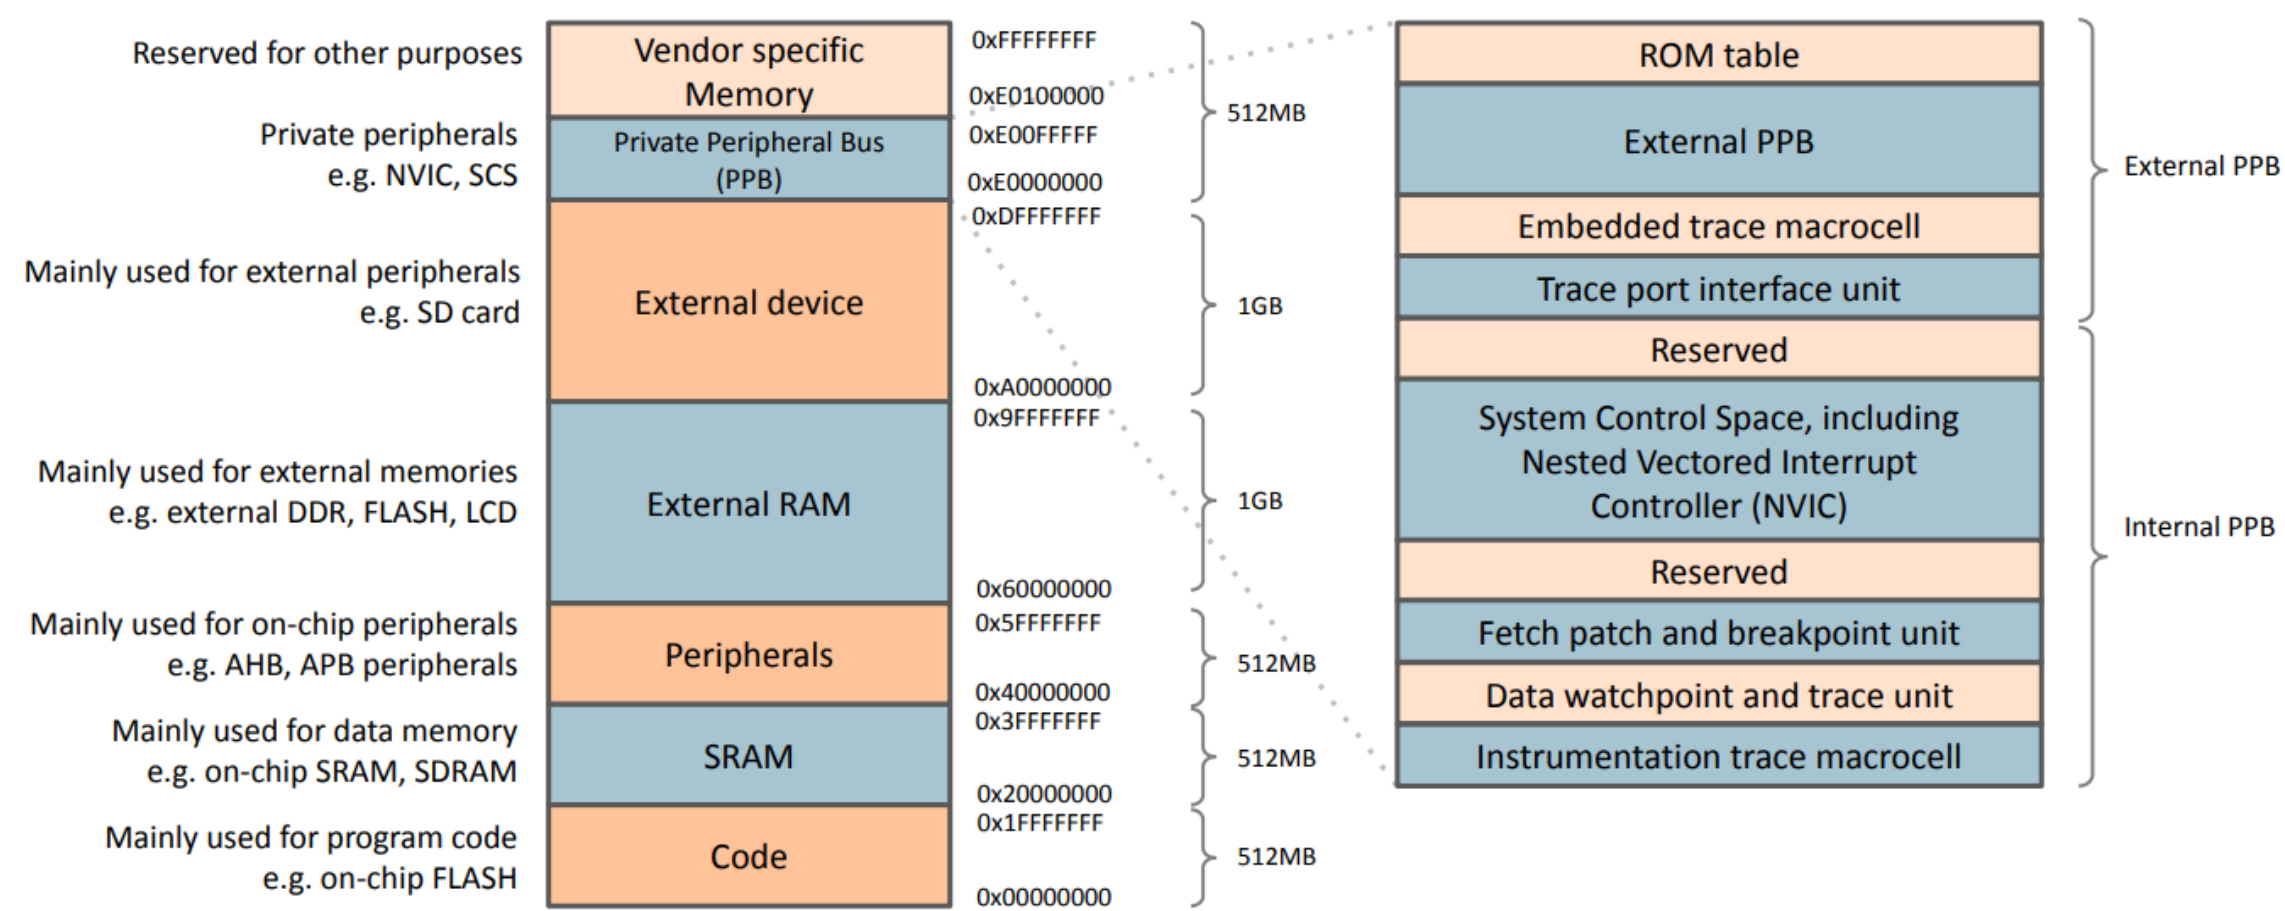
\includegraphics[width=1\linewidth]{img/image21.png}
\end{figure}


\paragraph{Code Region} It is primarily used to store program code, can also be used for data memory.
On-chip memory, such as on-chip FLASH.

\paragraph{SRAM Region} It is primarily used to store data, such as heaps and stacks. It can also be used to store program code.

\paragraph{Peripheral Region} It is primarily used for AHB/APB peripherals.
\paragraph{External RAM region} It is primarily used to store large data blocks or memory caches. It's an off-chip memory, slower than onchip SRAM region.
\paragraph{External device region} Used to map external, off-chip devices like SD cards.
\paragraph{Private Peripheral Bus (PPB)} Provides access to internal and external processor resources.


\section{Bit-band Operations}
One interesting property of Arm architectures is that they allow bit-band operations.

Bit-band operations allow a single load/store operation to access a single bit in the memory, without
having to access 32 bits at once just to change a single one.

It works by directly writing a single bit (0 or 1) to the "\textbf{bit-band alias address}" of the data.


\paragraph{Bit-band Alias Address}

SRAM and Peripheral regions include \textbf{bit band} and \textbf{bit band alias} areas.

\begin{figure}[H]
    \centering
    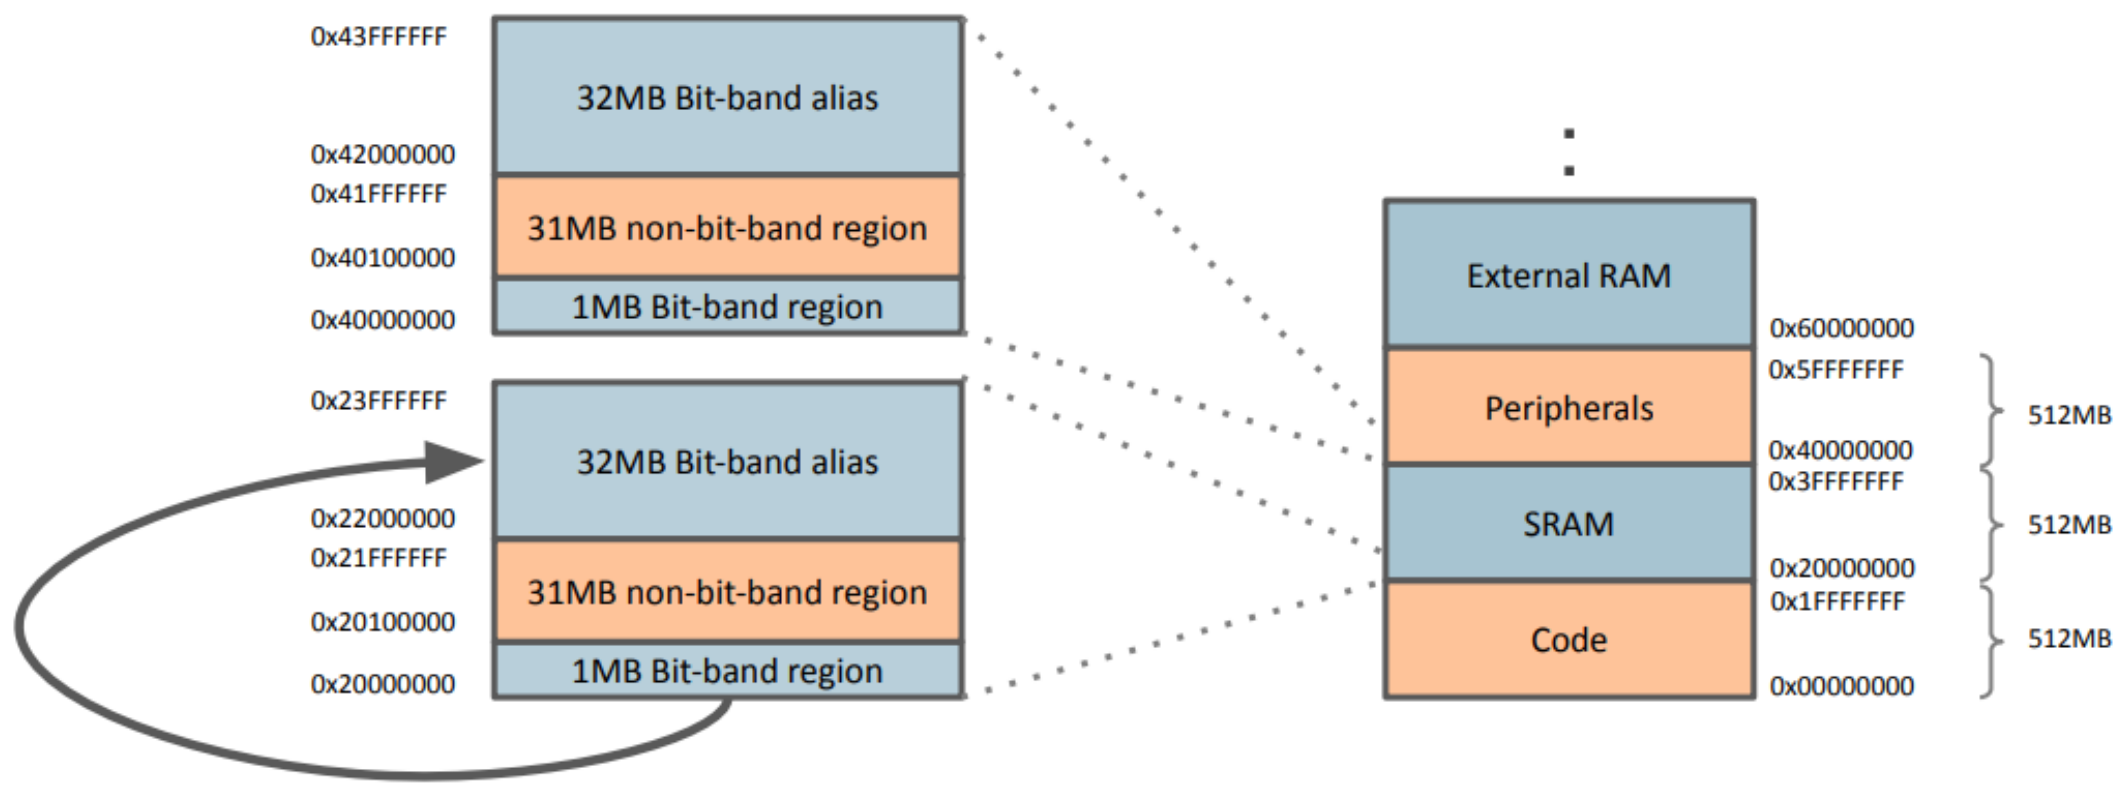
\includegraphics[width=1\linewidth]{img/image22.png}
\end{figure}

Each bit of the data is one-to-one mapped to the bit-band alias address. Each bit has an address multiple
of 4.


1 byte = 8 bits = 4x8 = 32 addresses in memory space.


\subsection{Benefits of bit-band operations}

Bit-band operations allow for \textbf{faster bit operations} and \textbf{fewer instructions}. It's an \textbf{atomic operation}, so it helps prevent data conflict hazards.

\newpage
\section{Cortex-M4 Endianness}

Endian refers to the order of bytes stored in memory.

\paragraph{Little endian:} lowest byte of a word-size data is stored in bit 0 to bit 7
\paragraph{Big endian: } lowest byte of a word-size data is stored in bit 24 to bit 31


Cortex-M4 supports both little endian and big endian. However, endianness only exists in the hardware level.


\begin{figure}[H]
    \centering
    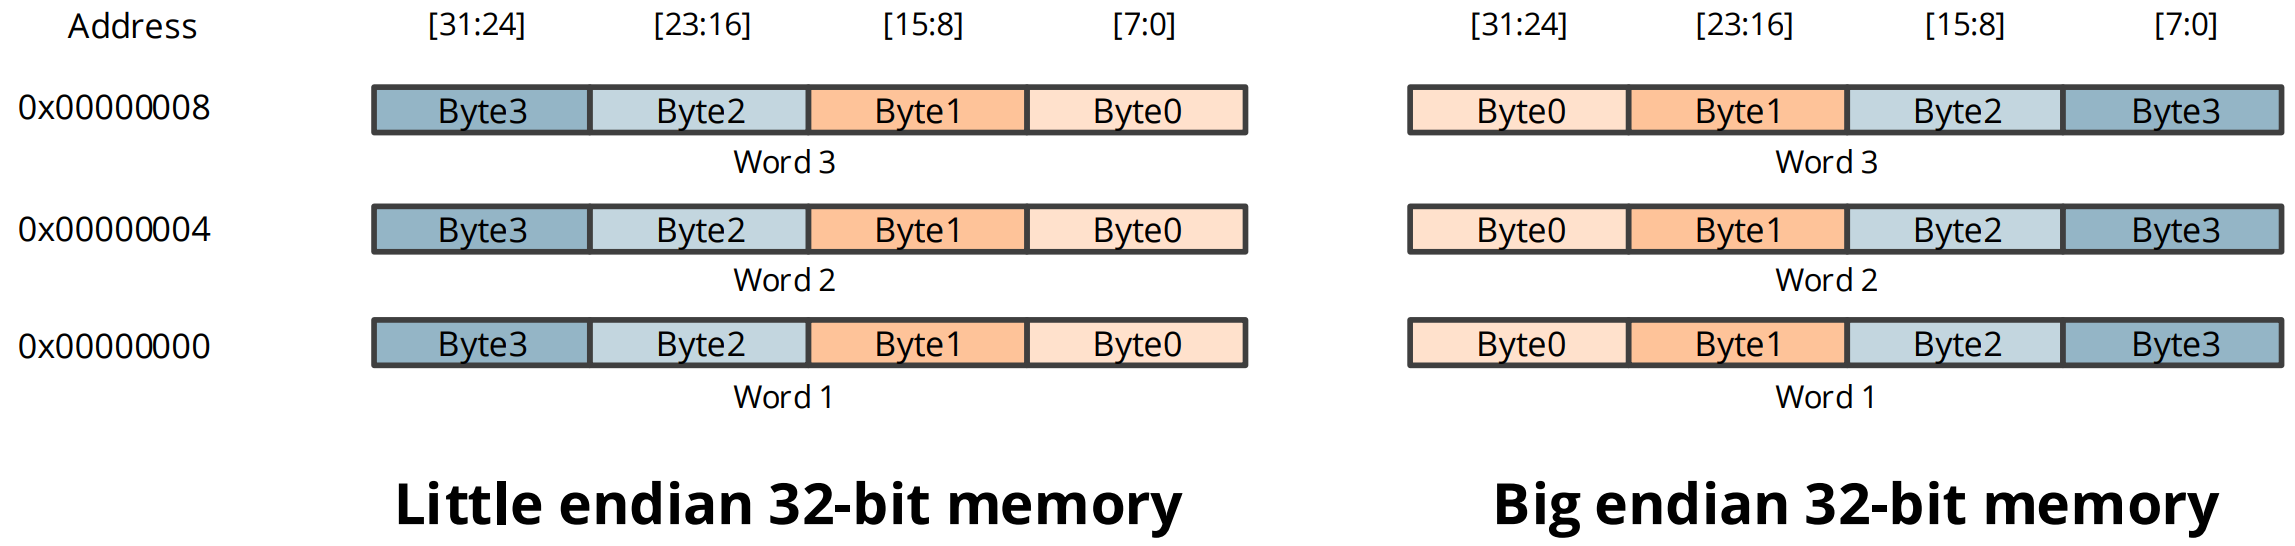
\includegraphics[width=1\linewidth]{img/image23.png}
\end{figure}


\section{Arm and Thumb Instruction Set}

The early Arm instruction set was a 32-bit instruction set called the Arm instructions. It's powerful and
performs well but it required a larger program memory and a larger power consumption.

\paragraph{Example: } ADDS Rd, Rd, \#Constant


\begin{figure}[H]
    \centering
    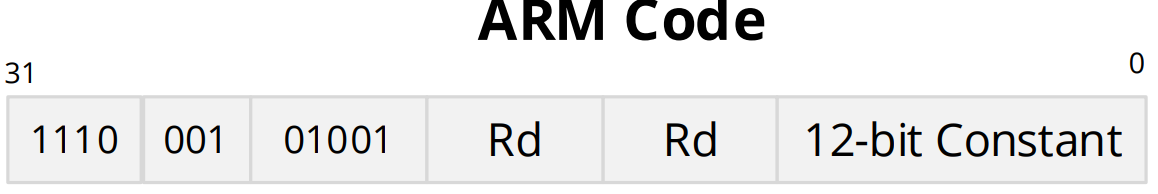
\includegraphics[width=0.7\linewidth]{img/image25.png}
\end{figure}

\paragraph{Thumb Code} ADD Rd, \#Constant


\begin{figure}[H]
    \centering
    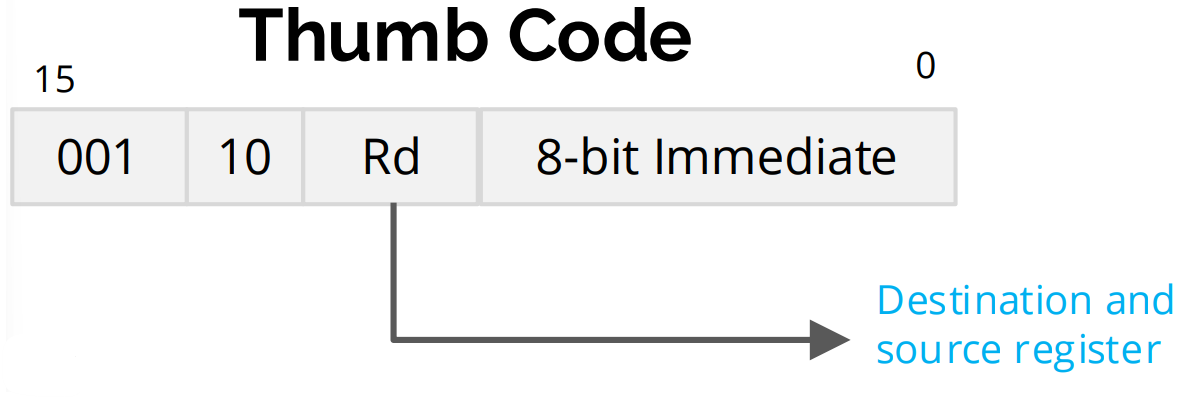
\includegraphics[width=0.6\linewidth]{img/image26.png}
\end{figure}

The instruction does the same operation but encoded using \textbf{less number of bits}!

\paragraph{}

Later on Arm introduced the Thumb-1 instruction set. It had 16-bit instructions as it was a subset of the
Arm instruction set.

\paragraph{}
Code size is reduced by -30\% but performance is also reduced by -20\%.

A multiplexer is used to switch between the two sets, which requires a switching overhead. This is so one
can benefit from 32-bit Arm's high performance and 16-bit Thumb-1's high code density (reduced program code size, Sometimes leads to an increased number of instructions, thus making thumb
slower to execute because fetching instructions is slower than executing instructions).

The processor
and the compiler manage this automatically.


\begin{figure}[H]
    \centering
    
\includegraphics[width=0.8\linewidth]{img/image27.png}
\end{figure}

\paragraph{The Thumb-2} instruction set consists of both 32-bit Thumb instructions and the original 16-bit Thumb-1
instruction sets. Compared to the 32-bit Arm instruction set, code size is reduced by -26\% with similar
performance.

The Thumb-2 instruction set also covers almost all functionality of the Arm instruction set and most
instructions are \textbf{unconditional}, whereas almost all Arm instructions are conditional.
\chapter{Program Development}

\section{Typical Program-generation Flow}

\begin{center}
    \textbf{Compile $\rightarrow$ Assemble $\rightarrow$ Link $\rightarrow$ Download.}
\end{center}


The generated executable file (or program image) is stored in the program
memory (normally an on-chip flash memory), to be fetched by the processor

\begin{figure}[H]
    \centering
    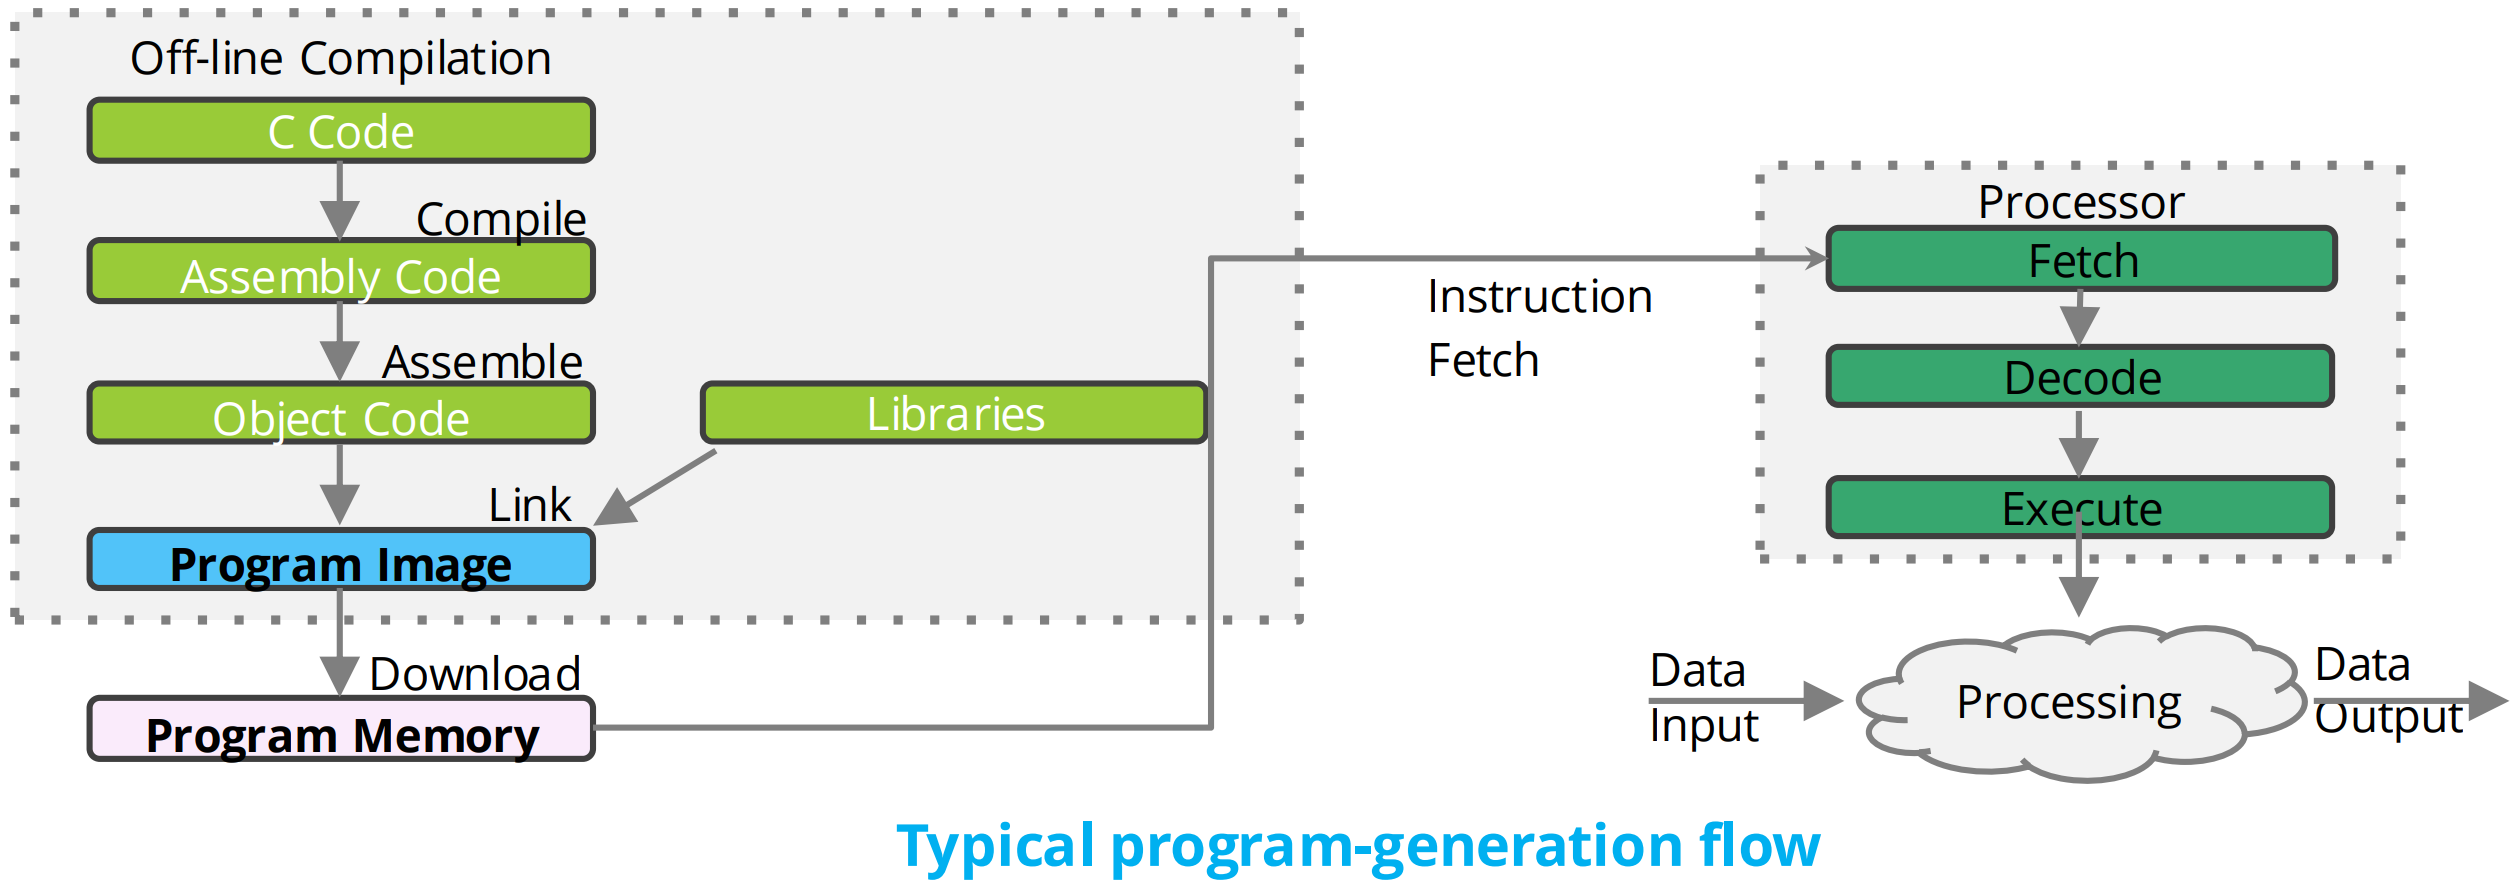
\includegraphics[width=0.85\linewidth]{img/image28.png}
\end{figure}

\section{Cortex-M4 Program Image}

A program image (or executable file) is a piece of fully integrated code that is ready to execute.


The program image includes :

 \begin{minipage}{\linewidth}
      \centering
      \begin{minipage}{0.40\linewidth}
            \begin{itemize}
                \item Program code
                \item C library code -> inserted by the linker
                \item Vector table : contains the starting addresses of interrupt vectors and the MSP (\textbf{main stack point})
                \item C startup code : used to set up data memory and initialize global variables
            \end{itemize}
      \end{minipage}
      \hspace{0.05\linewidth}
      \begin{minipage}{0.45\linewidth}
          \begin{figure}[H]
                \centering
                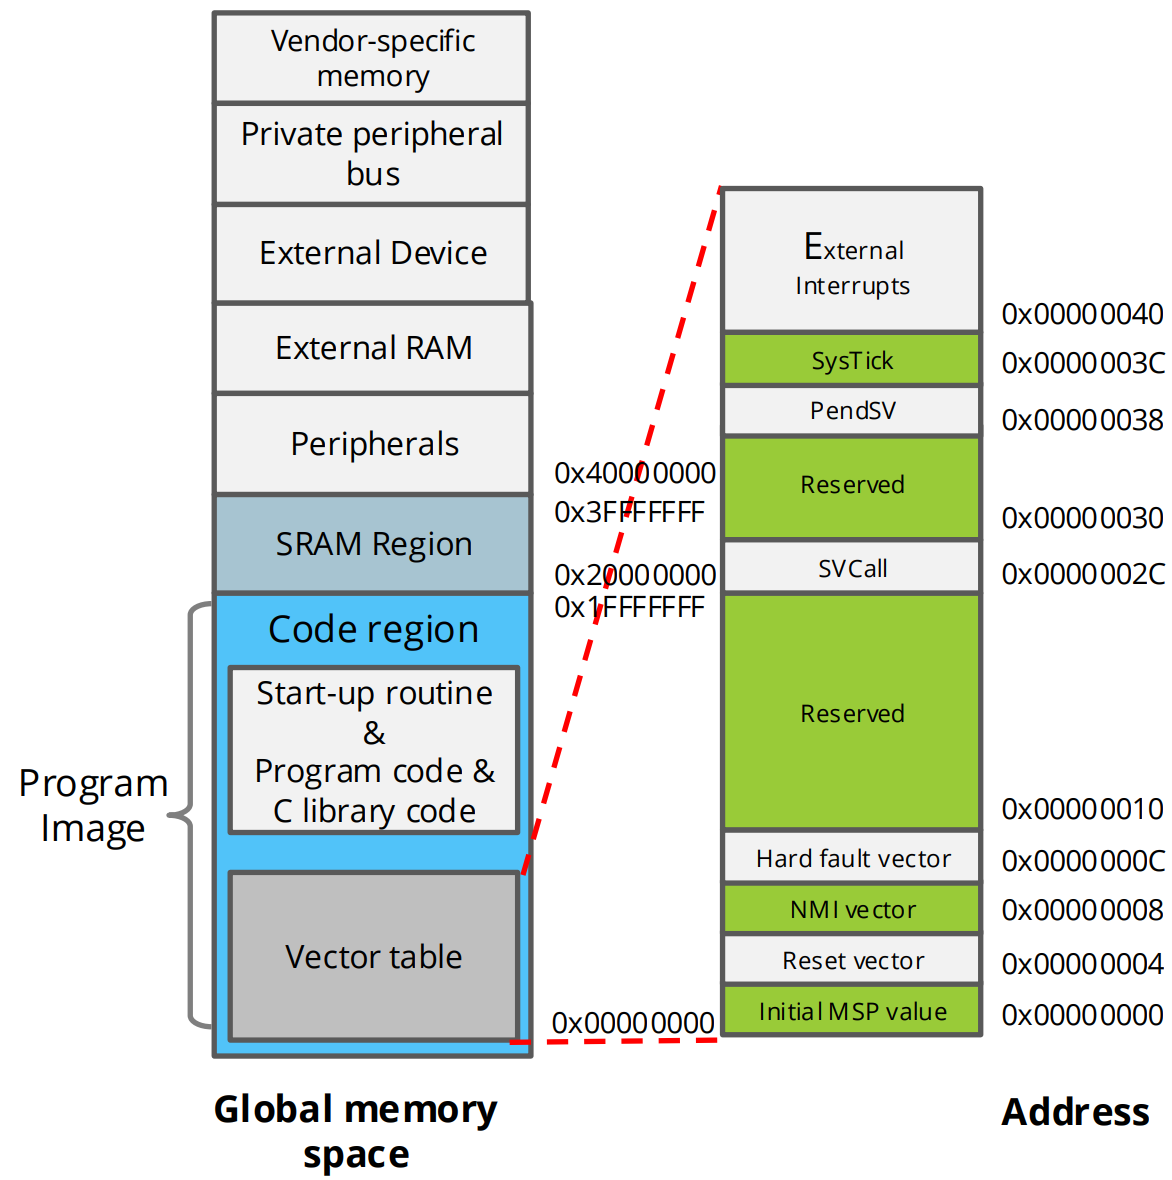
\includegraphics[width=1\linewidth]{img/image29.png}
          \end{figure}
      \end{minipage}
  \end{minipage}


\subsection{Systems Initialization}

When the system resets:

\begin{figure}[H]
    \centering
    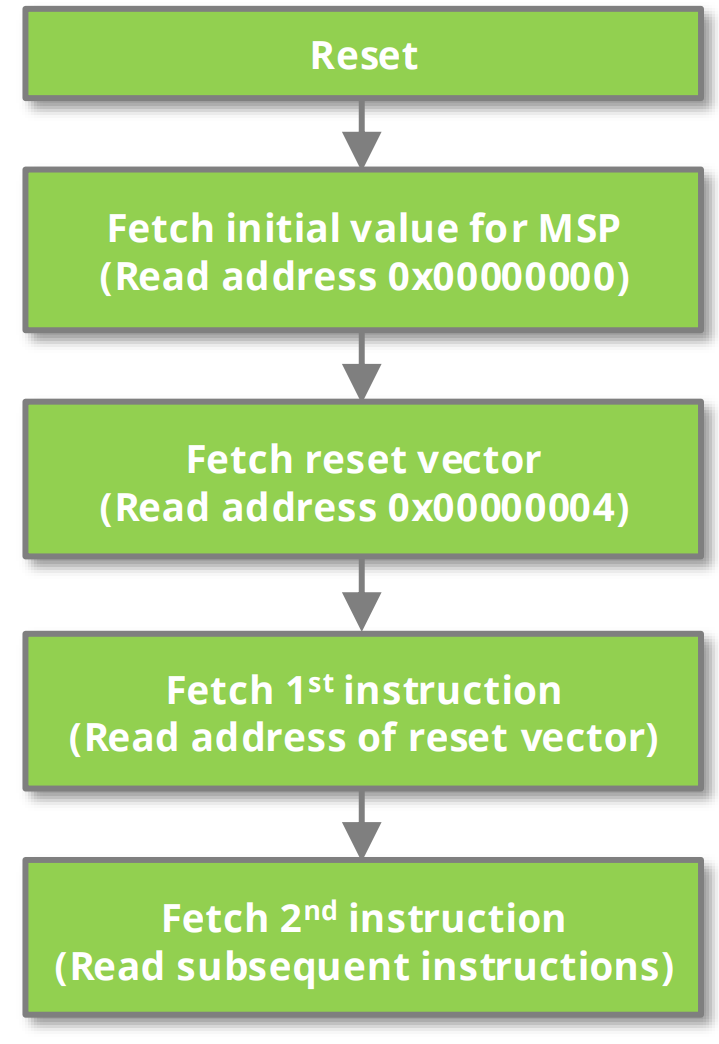
\includegraphics[width=0.23\linewidth]{img/image30.png}
\end{figure}

\section{Program Image in Global Memory}

The \textbf{program image} is stored in the code region in global memory and occupies at most 511 MB of data.

It is usually implemented on \textbf{non-volatile memory}, such as on-chip flash memory.

The executable image contains initialized data and uninitialized data. Normally separated from program data, which is allocated in the SRAM region (or data region)


\begin{figure}[H]
    \centering
    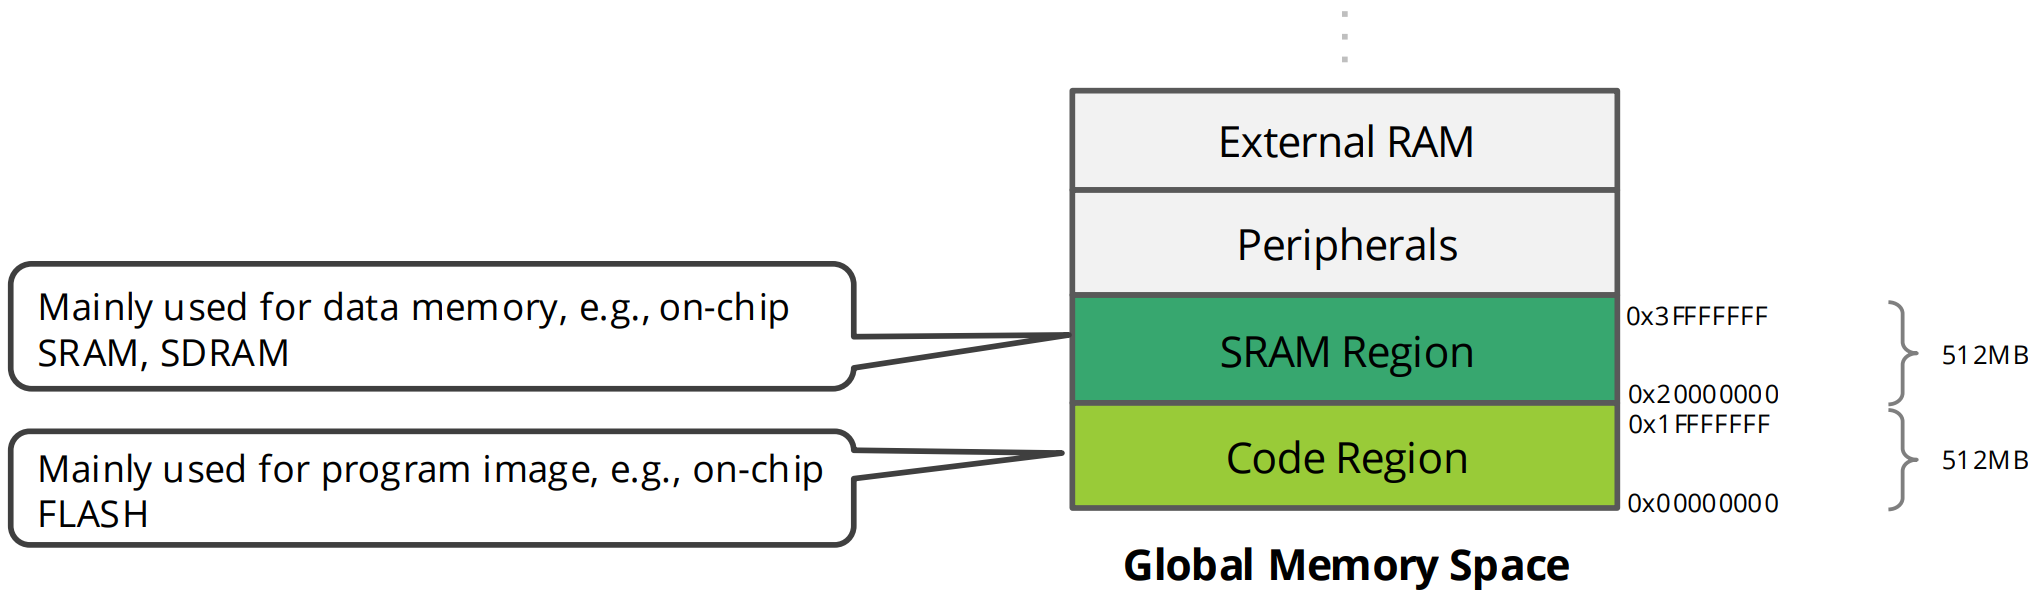
\includegraphics[width=0.8\linewidth]{img/image31.png}
\end{figure}

Normally separated from program data, which is allocated in the SRAM
region (or data region)

\section{How is Data Stored in RAM?}

Typically, the data can be divided into three
sections: \textbf{static data}, \textbf{stack}, and \textbf{heap}

 \begin{minipage}{\linewidth}
      \centering
      \begin{minipage}{0.40\linewidth}
          \begin{itemize}
            \item \textbf{Static data}: global variables and static variables
            \item \textbf{Stack}: local variables, parameter passing in function calls, registers saving during exceptions, etc.
            \item \textbf{Heap}: pieces of memory spaces that are dynamically reserved by function calls, such as ‘alloc()’ and ‘malloc ()’. (Generally not preferred in embedded systems)
        \end{itemize}
      \end{minipage}
      \hspace{0.05\linewidth}
      \begin{minipage}{0.35\linewidth}
          \begin{figure}[H]
                \centering
                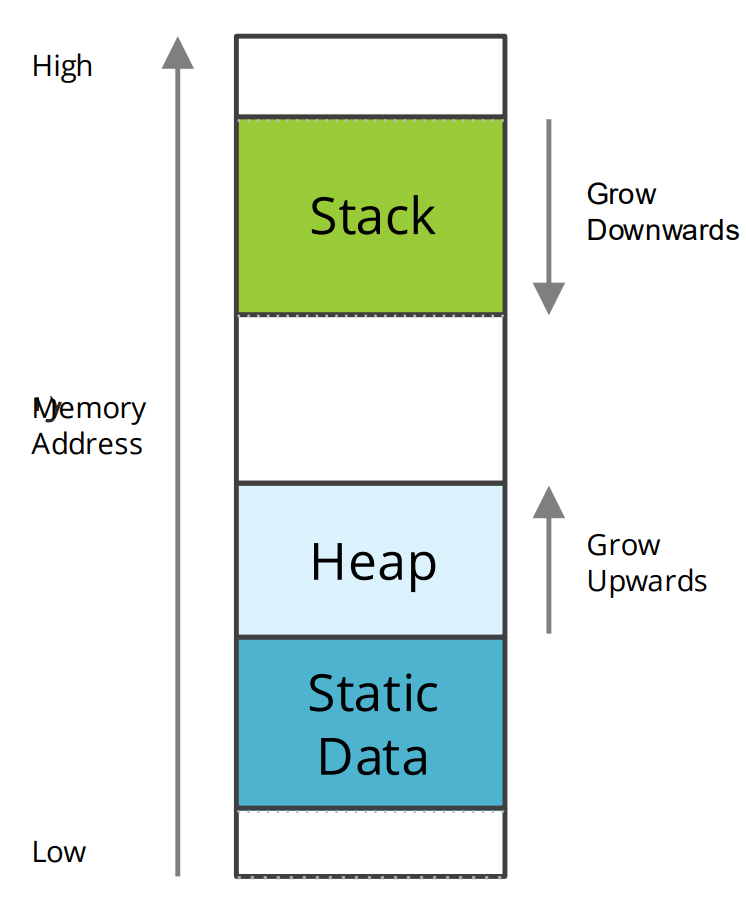
\includegraphics[width=1\linewidth]{img/image33.png}
          \end{figure}
      \end{minipage}
  \end{minipage}


\subsection{How to decide on the use of memory to store data?}

\paragraph{Information do not change: } Put it in read-only nonvolatile memory, e.g. Instructions, Constant strings, Constant
operands,
Initialization values...

\paragraph{Information change: } Put it in read/write memory, e.g. Variables, Intermediate computations,
Return address.

\begin{center}
    

\begin{lstlisting}[language=c++]
int a, b;
const char c=123; //heap
int d=31;

void main(void) {
    int e;
    char f[32];
    e = d + 7;
    a = e + 29999; //immediate value
    strcpy(f,"Hello!");
}
\end{lstlisting}
\end{center}

\begin{figure}[H]
    \centering
    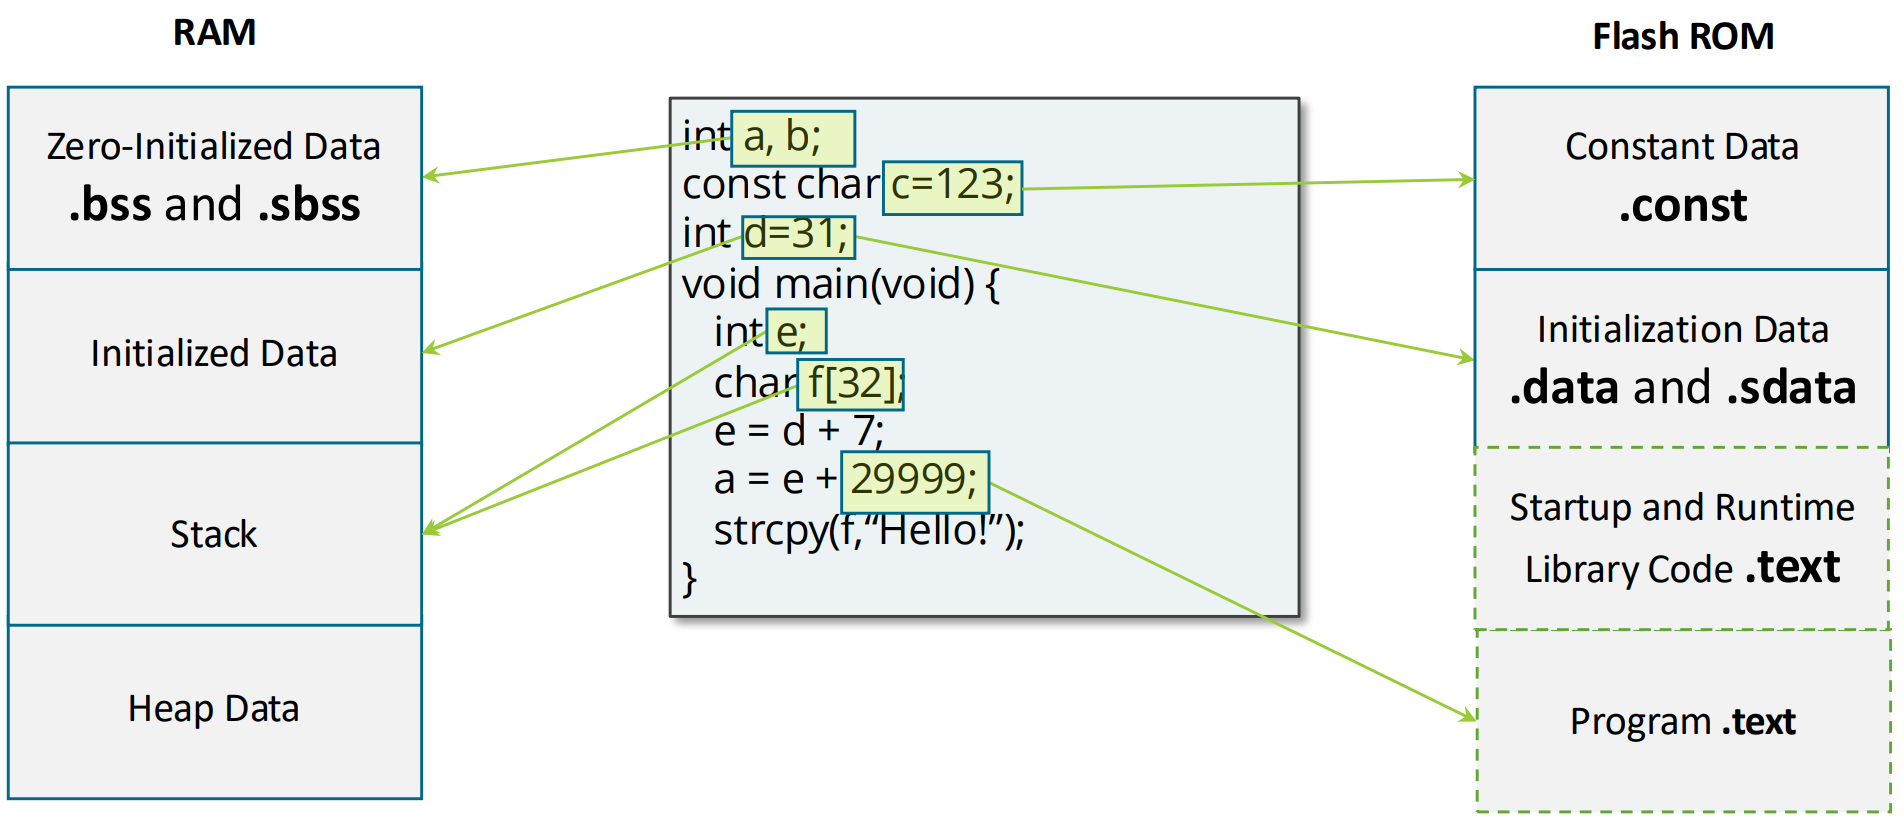
\includegraphics[width=0.85\linewidth]{img/image34.png}
\end{figure}


Executable image contains \textbf{initialized} data and \textbf{uninitialized} data sections:

\begin{itemize}
    \item .data and .sdata: contain the initial values for the global and static variables
    \item .bss and .sbss: uninitialized (or zero initialized) data sections (their content is empty)
    \item .const: constant data is part of the.const section which is read-only.
\end{itemize}


\subsection{C Run-Time Start-Up Module}

 \begin{minipage}{\linewidth}
      \centering
      \begin{minipage}{0.40\linewidth}
          After reset, MCU must: Initialize hardware... and Initialize C or C++ runtime environment: Set up heap memory, Initialize variables.
      \end{minipage}
      \hspace{0.05\linewidth}
      \begin{minipage}{0.35\linewidth}
          \begin{figure}[H]
                \centering
                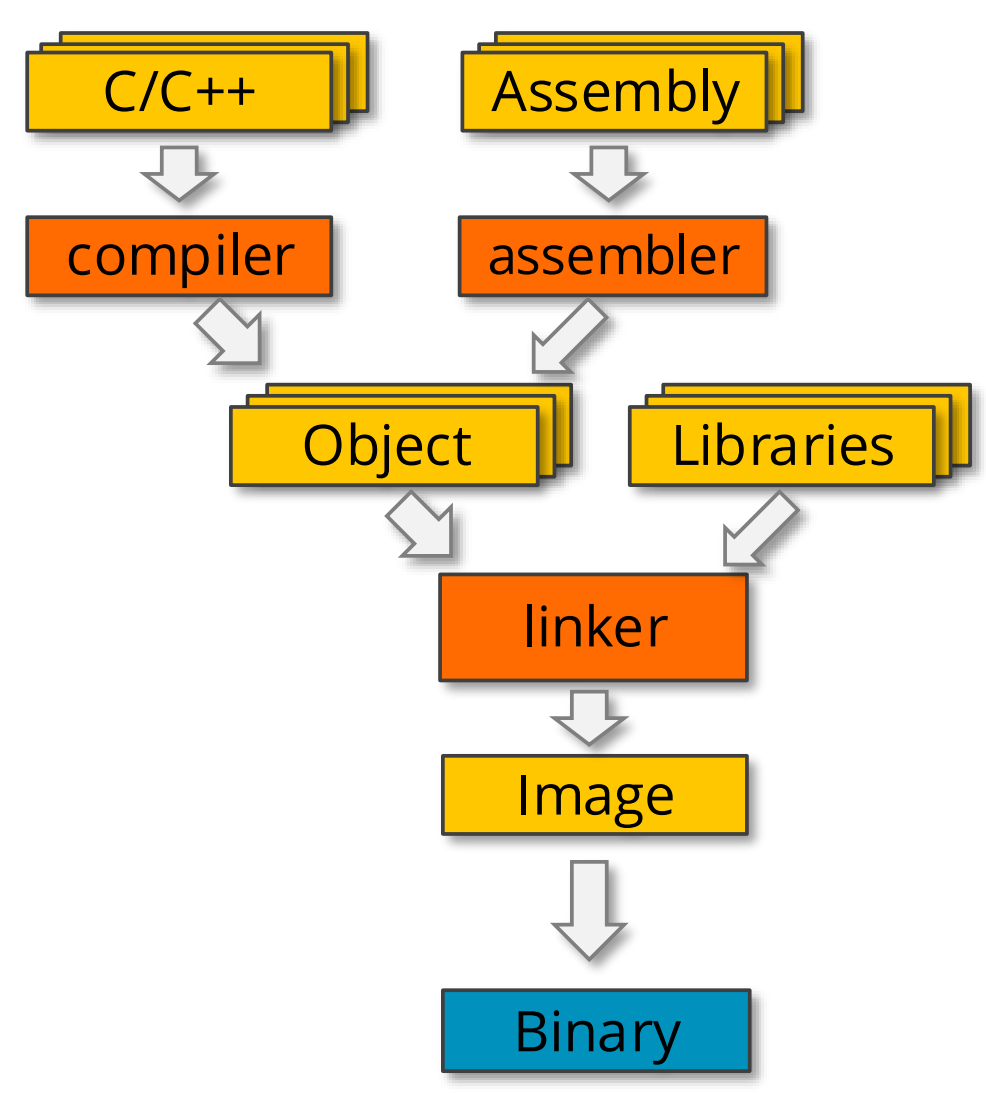
\includegraphics[width=1\linewidth]{img/image35.png}
          \end{figure}
      \end{minipage}
  \end{minipage}
  
\section{load the program mage into the target (microcontroller)}

To load a program image, we need to transfer the executable image from the host to the target (for example through an USB Cable).

There are 3 steps :

\begin{enumerate}
    \item Creating a program image in the host
    \item Loading the program image in the microcontroller using special equipment like JTAG
    \item Executing the program in the microcontroller
\end{enumerate}


\paragraph{Step one: } The linker create a single executable image for the target embedded system. 

The linker directives control how the linker combines the sections and allocates the segments into the
target system. 
Two of the more common linker directives are:

\begin{itemize}
    \item \textbf{MEMORY} : used to describe the target system's memory map, types of physical memory and address range occupied by each physical memory block
    \item[] \begin{minipage}{\linewidth}
      \centering
      \begin{minipage}{0.40\linewidth}
          \begin{figure}[H]
                \centering
                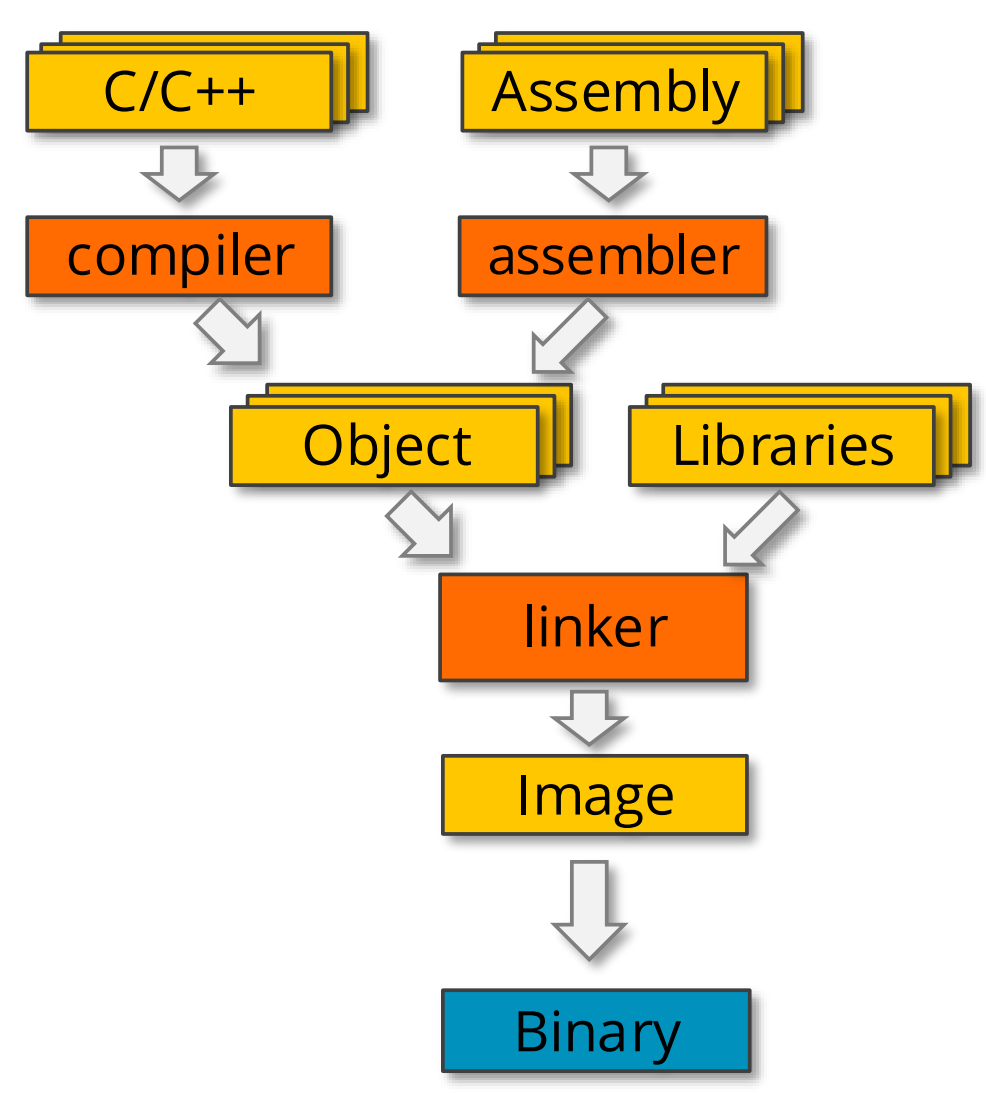
\includegraphics[width=1\linewidth]{img/image35.png}
          \end{figure}
      \end{minipage}
      \hspace{0.05\linewidth}
      \begin{minipage}{0.35\linewidth}
          \begin{figure}[H]
                \centering
                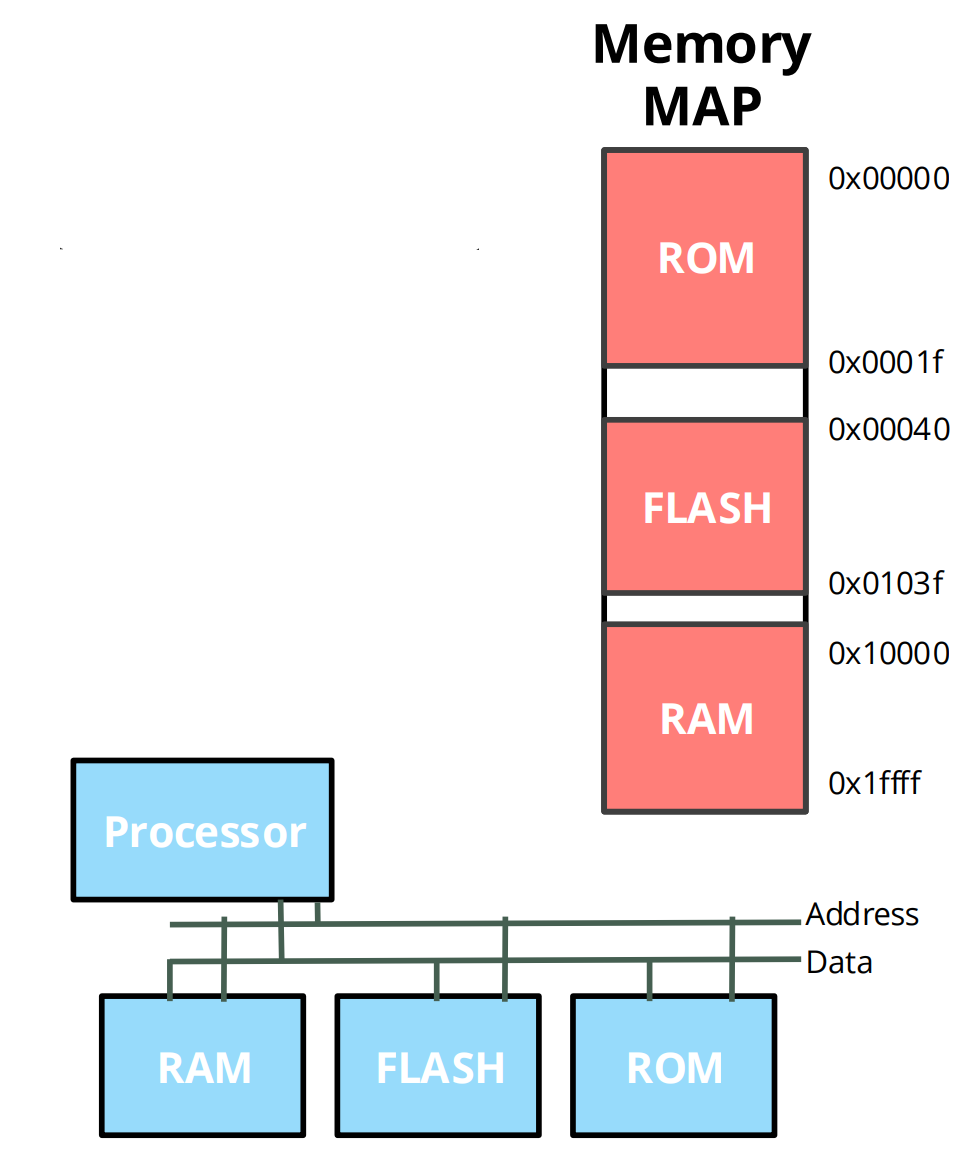
\includegraphics[width=1\linewidth]{img/image36.png}
          \end{figure}
      \end{minipage}
  \end{minipage}
  
    \item \textbf{SECTION} tells the linker:
    \begin{itemize}
    \item which input sections are to be combined into which output section
    \item which input sections are grouped together and allocated in contiguous memory
    \item where to place each section
    \end{itemize}
\end{itemize}


  \begin{figure}[H]
      \centering
      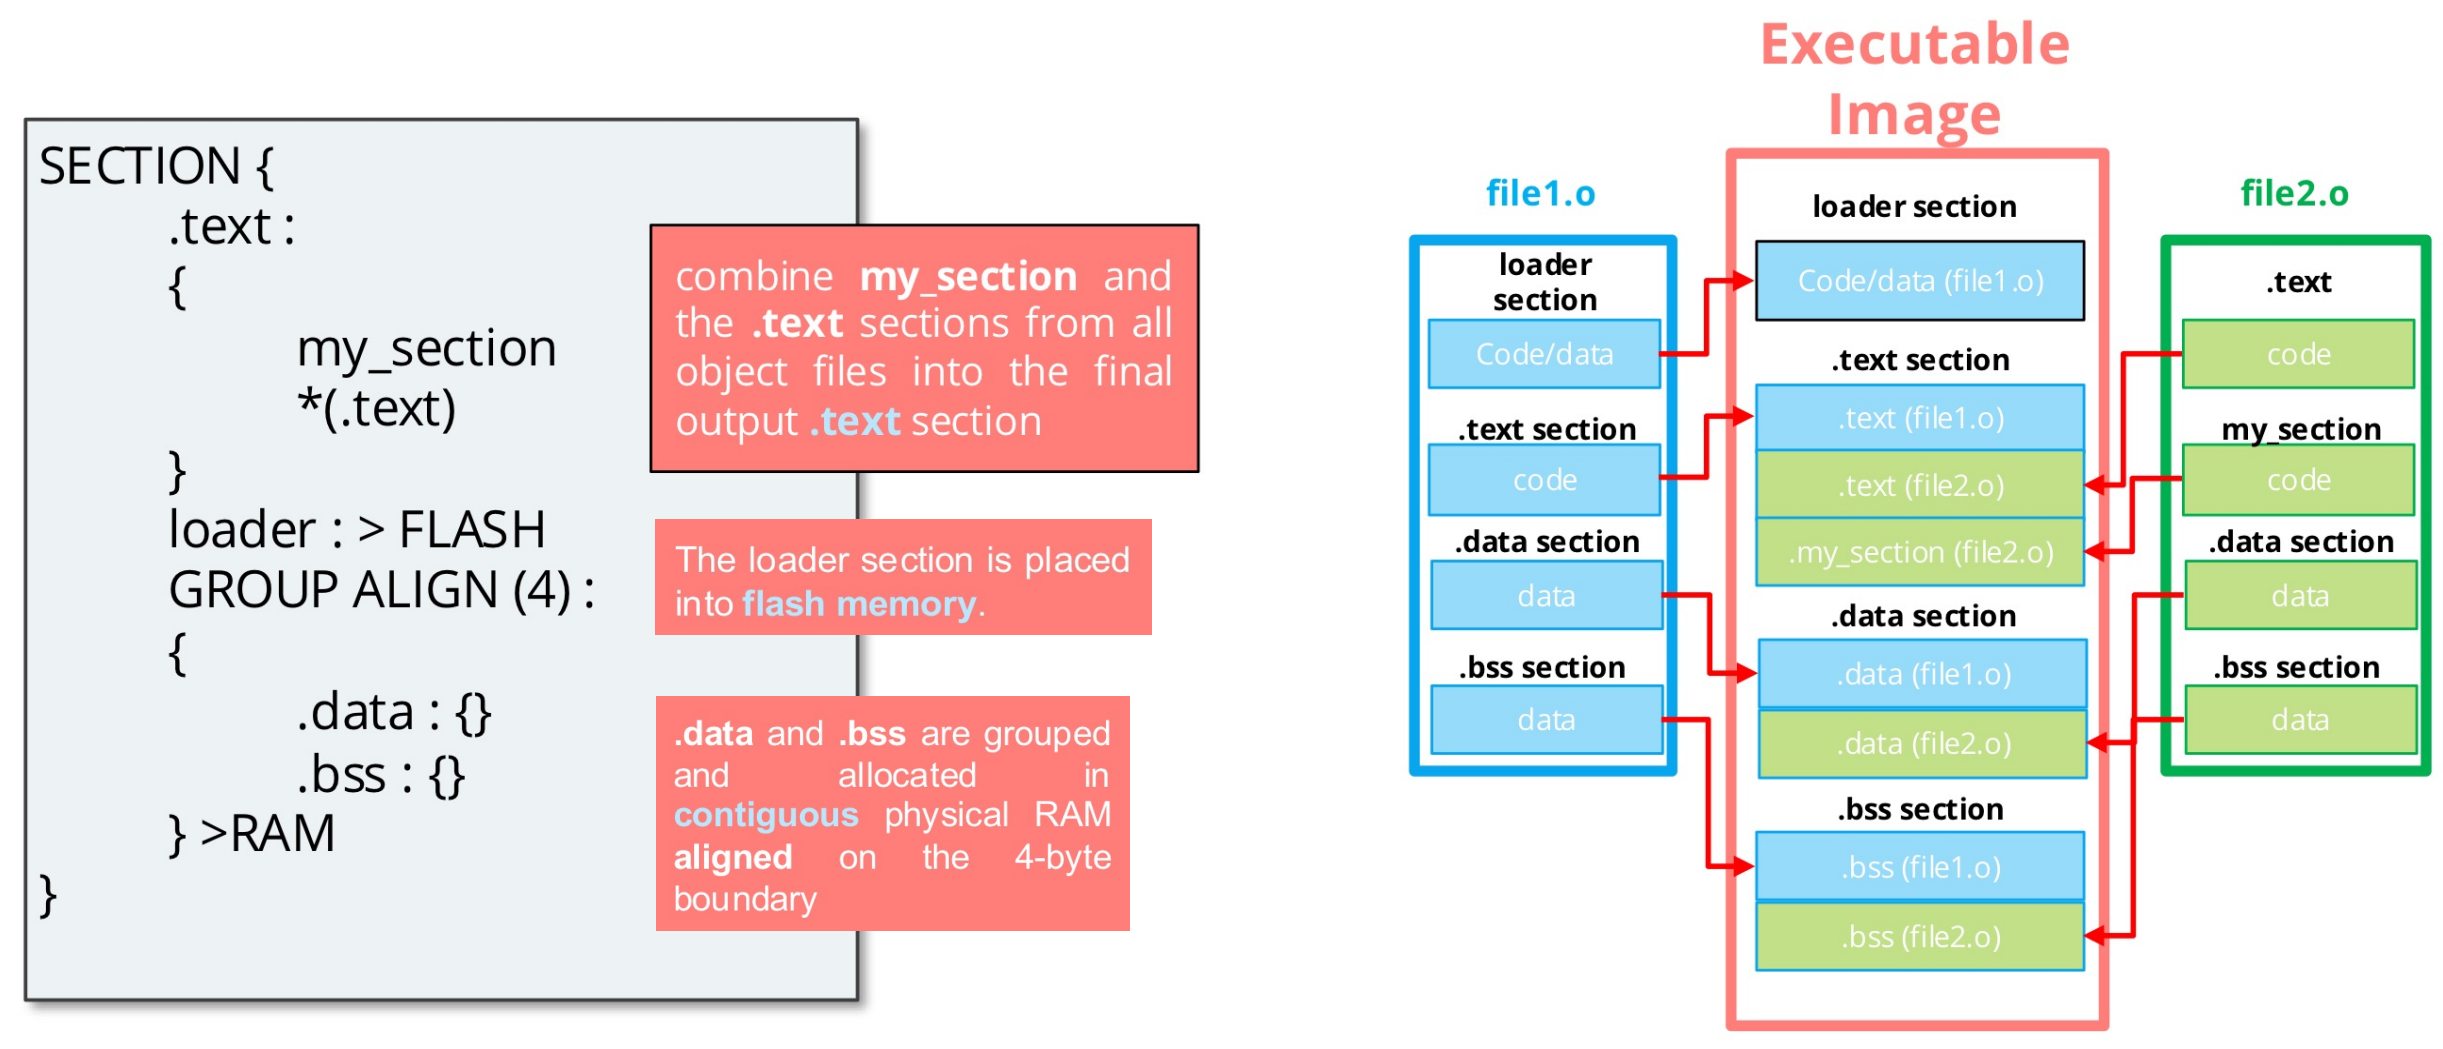
\includegraphics[width=0.9\linewidth]{img/image38.png}
  \end{figure}

  

\paragraph{Step two: }

After powered on,
the target executes code from a predefined address offset. The code in this memory location is called reset vector,
which is typically a jump instruction into the bootstrap code.

\paragraph{}
During booting, two CPU registers are concerned:

\begin{itemize}
    \item The instruction pointer register points to the next instruction (IP)
    \item The stack pointer points to the next free location in stack (SP)
\end{itemize}


\begin{figure}[H]
    \centering
    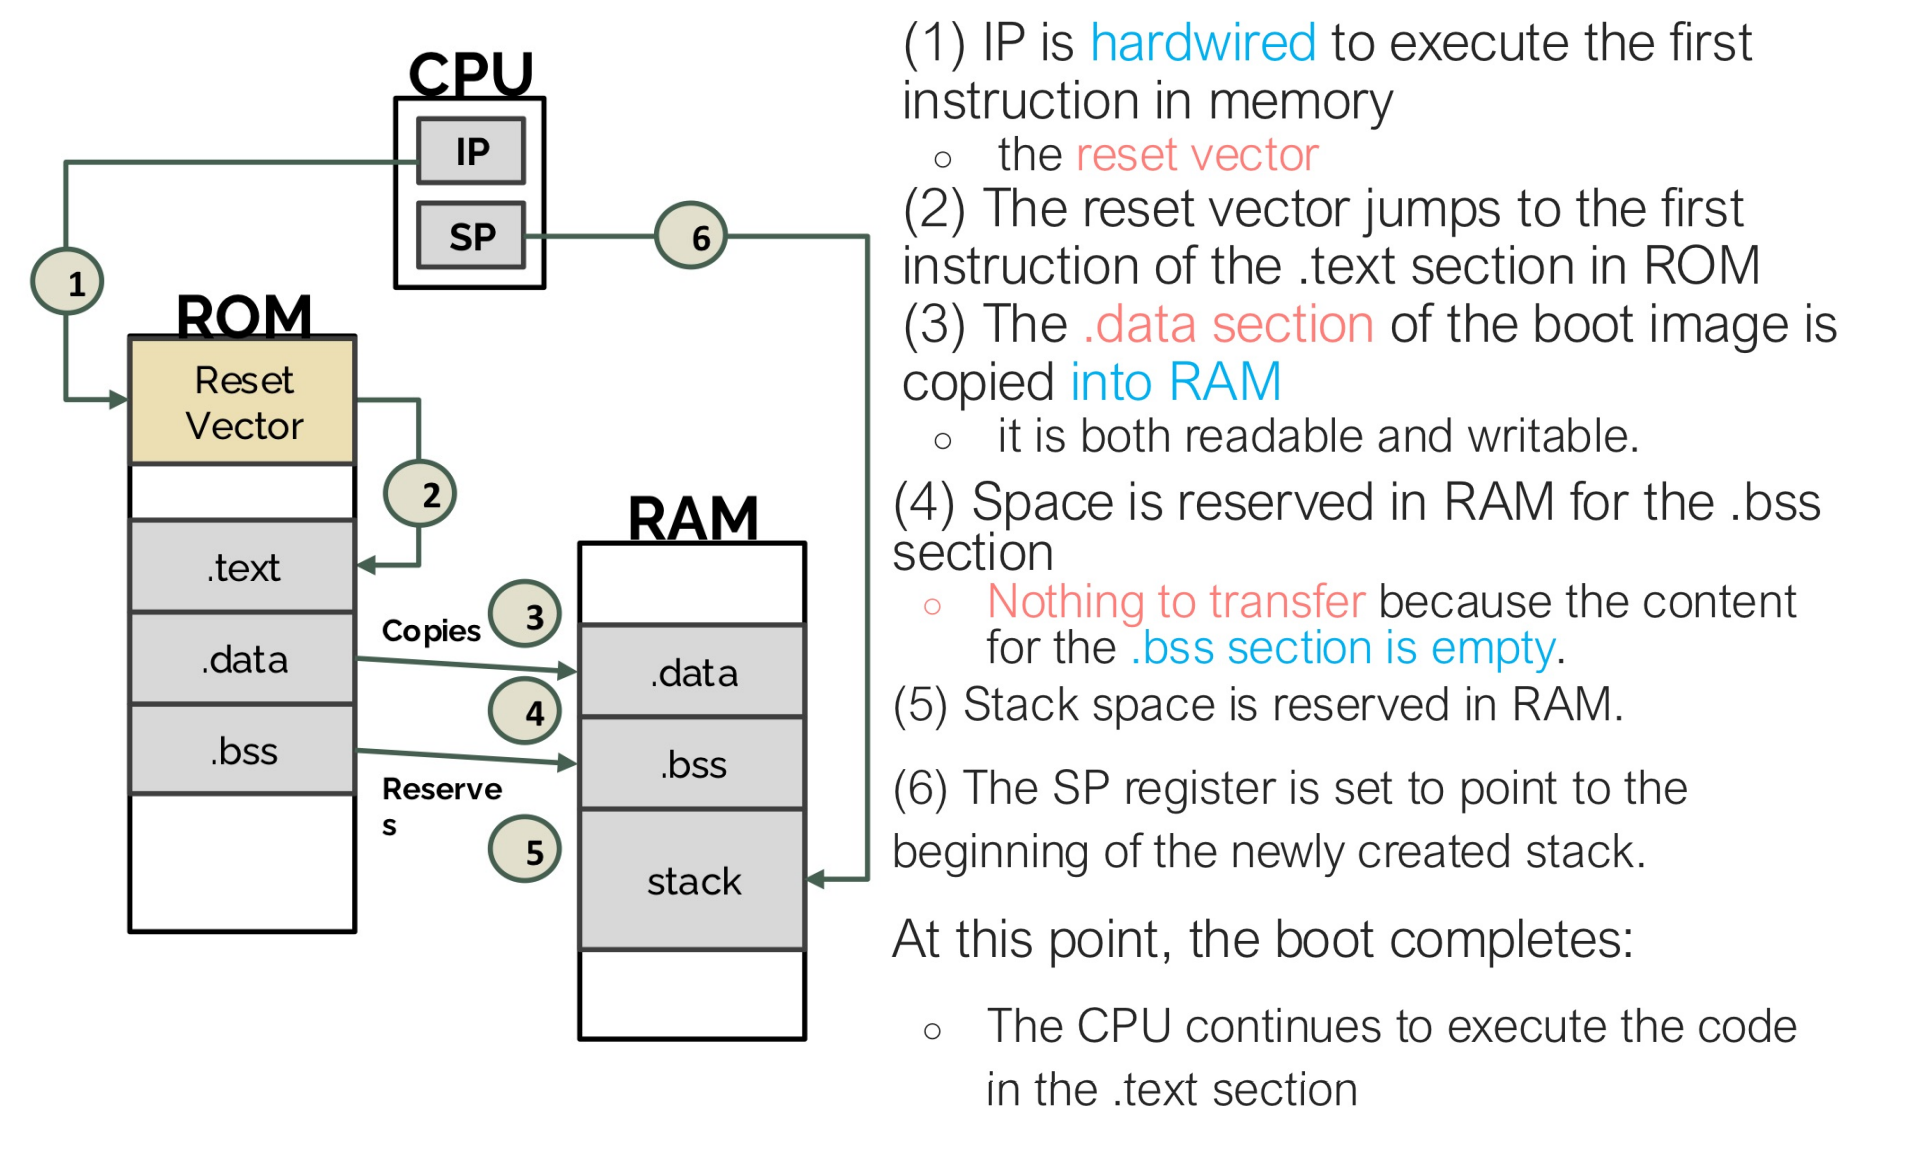
\includegraphics[width=0.9\linewidth]{img/image37.png}
\end{figure}
\chapter{IO Operations, Interrupts, and Their Impact on Embedded Systems}

\begin{figure}[H]
    \centering
    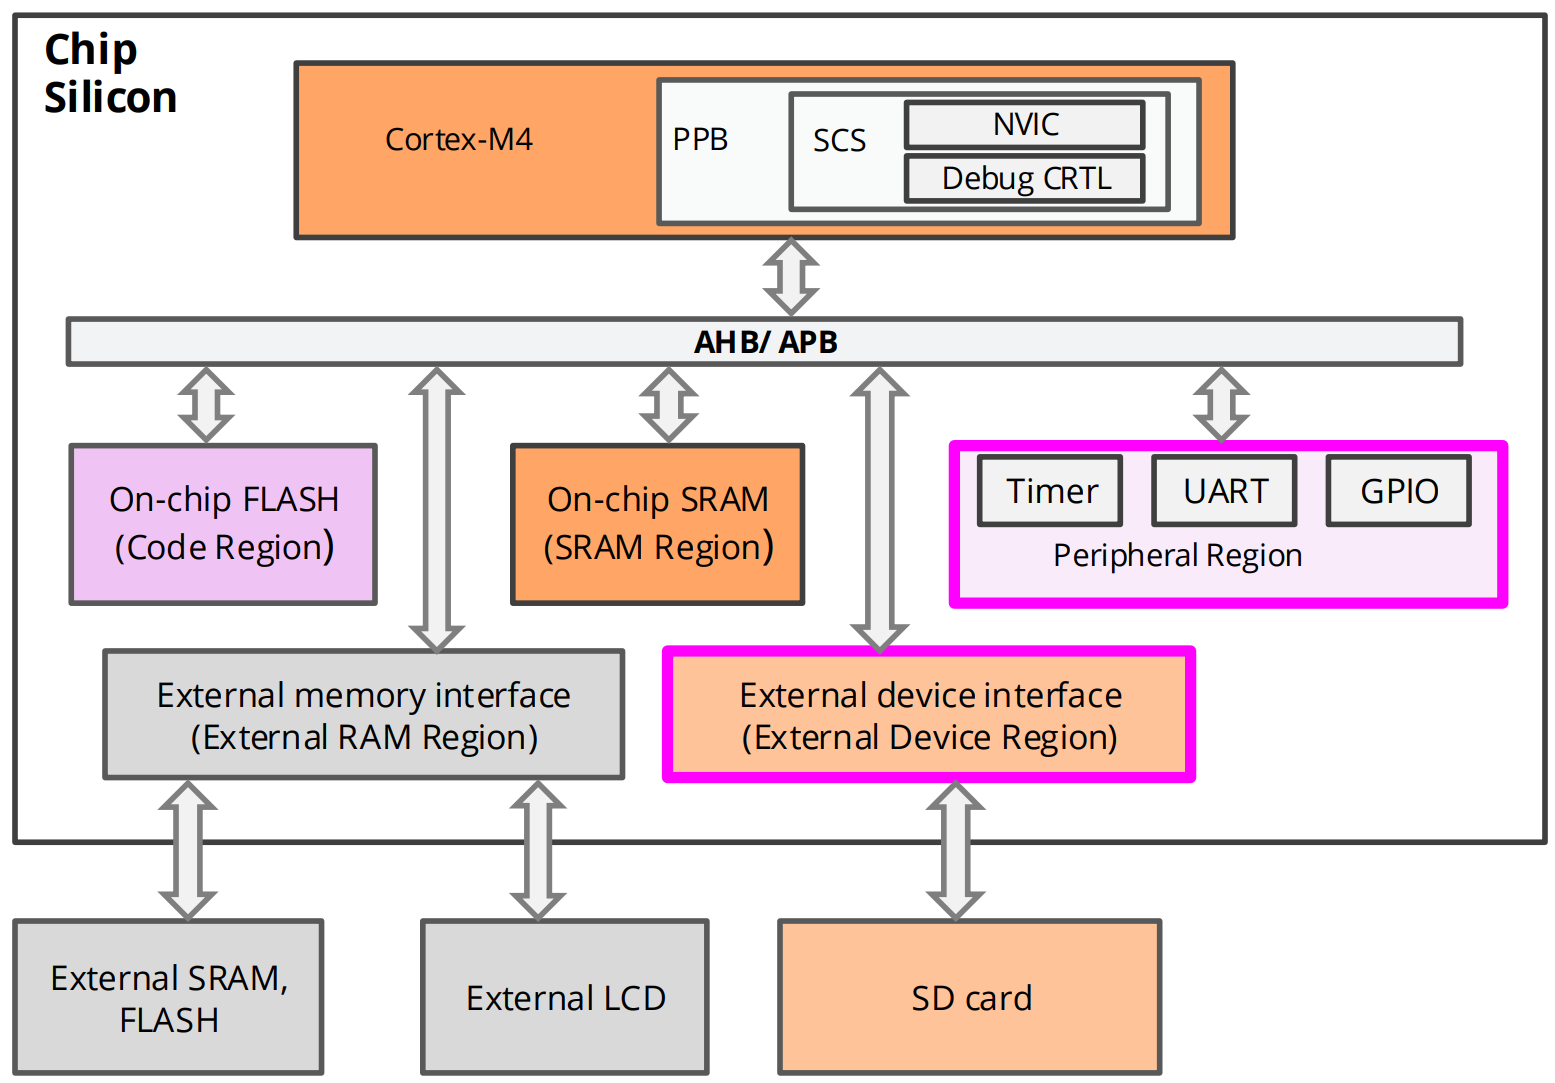
\includegraphics[width=0.8\linewidth]{img/image40.png}
    \caption{Input and Output Devices}
\end{figure}

\section{Current state of Art}
Currently Arm architecture dominates the embedded market. But there is a trend of switching to RISC-V.


\paragraph{}
The benefits is that RISC-V is open-source and more customisable. Because it's open-source this means
it's cheaper to develop with as there are no licensing fees or royalties to pay. ARM is dominant in the
embedded device market but RISC-V is getting more and more use in research and niche markets,
allowing reduced vendor lock-in and greater innovation.

\paragraph{}
\textbf{ARM} processors seem to be more \textbf{power-efficient} for now. \textbf{RISC-V's ecosystem} is growing but it \textbf{is not as
mature and rich as ARM's.}

\newpage
\section{Programming Input and Output}

The CPU talks to the device by reading and writing device registers.

\begin{figure}[H]
    \centering
    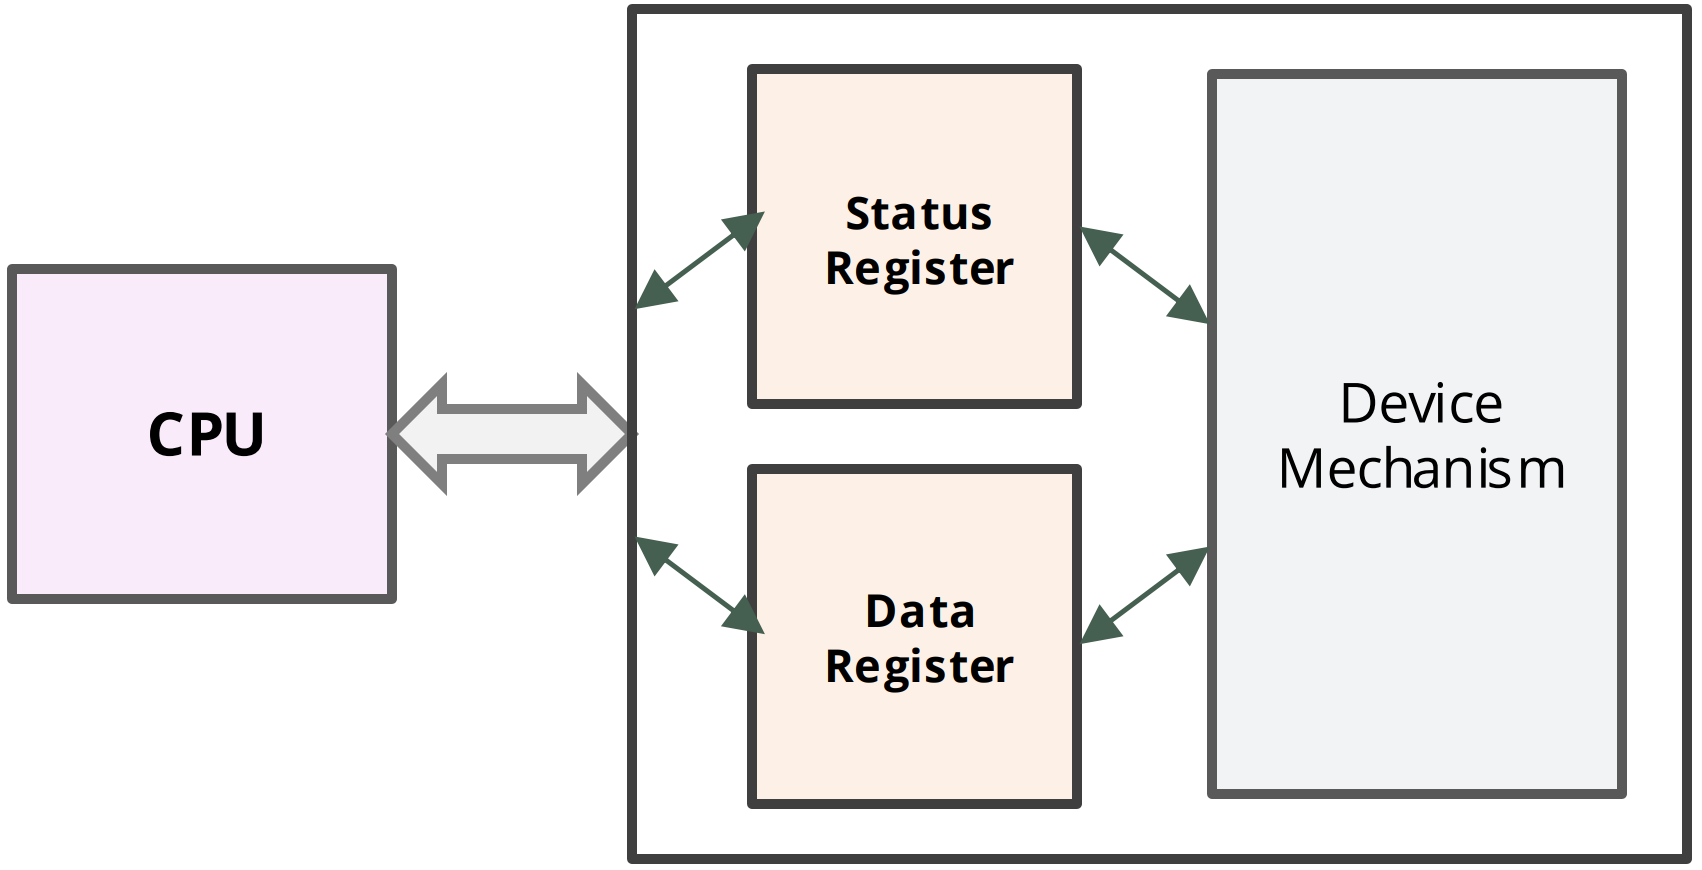
\includegraphics[width=0.6\linewidth]{img/image41.png}
\end{figure}

Devices typically have several registers:

\begin{itemize}
    \item[-] Data registers: hold data values, can be \textbf{readable or writable};
    \item[-] Status registers: provide information about the device's operation, can be \textbf{read-only}
\end{itemize}


\subsection{How to access the registers}

There are two way to access those registers:

\begin{itemize}
    \item[] \textbf{I/O instructions:} special instructions for input (read) and output (write) (in and out in case of Intel x86), requires a separate address space for each I/O device
    \item[] \textbf{Memory-mapped I/O:} the registers are mapped to the memory space of the device, meaning that we will need to manipulate the dedicated registers via normal memory read and write to communicate with devices. Very simple way.
\end{itemize}

We will use memory-mapped I/O throughout the course.


\subsection*{Example: Memory-mapped I/O on ARM}

Define location for device and provide Read/Write code:

\begin{lstlisting}[language=c++]
    DEV1 EQU 0x1000
    LDR r1,#DEV1 ; set up device addres
    LDR r0,[r1] ; read DEV1
    LDR r0,#8 ; set up value to write
    STR r0,[r1] ; write value to device
\end{lstlisting}


\subsection*{Example: write I/O in C}

We can use pointers to manipulate the addresses of I/O devices

\begin{lstlisting}[language=c]
    int read(char *location) {
        return *location;
    }
    void write(char *location, char newval) {
        (*location) = newval;
    }

\end{lstlisting}

To read a device register we can write:

\begin{lstlisting}[language=c]
    #define DEV1 0x1000
    ...
    dev_status = read(DEV1); /* read device register */
\end{lstlisting}

To write to the status register, we can use the following code:

\begin{lstlisting}[language=c]
    write(DEV1,8); /* write 8 to device register */
\end{lstlisting}


\section{Busy-Wait I/O}

Devices are typically slower than the CPU, so they may require many cycles to complete an operation.

The Busy-Wait, a.k.a. polling,  is a technique in which the CPU keeps asking the I/O
device if it has finished the operation by checking its status register.

\subsubsection{Example: Busy-Wait I/O}

We need to write a sequence of characters to an output device. The device has two registers, one for the
character to be written and a status register.

The status register's value is 1 when the device is busy writing and 0 when the write has completed.


\begin{lstlisting}[language=C]

    #define OUT_CHAR 0x1000 /* output device character register */
    #define OUT_STATUS 0x1001 /* output device status register */
    ...
    char *mystring = "Hello, world." /* string to write */
    char *current_char; /* pointer to the current position in string */
    current_char = mystring; /* point to the head of string */
    while (*current_char != '\0') { /* until null character */
        write(OUT_CHAR,*current_char); /* send character to device */
        while (read(OUT_STATUS) != 0); /* keep checking status */
        current_char++; /* update character pointer */
    }   
\end{lstlisting}

As shown in the example, we write one character each then check if the device has finished writing to
send the next one.

\paragraph{}
When a new character has been read: the input device sets its status register to 1, we must set it back to 0 so that the device is ready to read another character 

\paragraph{}To start writing: first set the output status register to 1, then wait for it to return to 0.

\subsubsection{Example 2: Busy-Wait I/O}
The following example showcases a simple application involving an input device and an output device
connected to the same CPU.

\begin{lstlisting}[language=C]

    #define IN_DATA 0x1000
    #define IN_STATUS 0x1001
    #define OUT_DATA 0x1100
    #define OUT_STATUS 0x1101
    ...
    while (TRUE) { /* perform operation forever */
    /* read a character into achar */
    
    while (read(IN_STATUS) == 0); /* wait until ready */
        achar = (char)read(IN_DATA); /* read the character */
        write(OUT_DATA,achar); /* write achar */
        write(OUT_STATUS,1); /* turn on device */
        while (read(OUT_STATUS) != 0); /* wait until done */
    }   
\end{lstlisting}

The code is supposed to get input from a keyboard and then show it onto an LCD display:

\begin{itemize}
    \item[-] It keeps waiting until the input device's status is set to ready, indicating a new character
    \item[-] It reads the new character and stores it in memory
    \item[-] It writes the new character in the data register of the output device
    \item[-] It keeps waiting until the output device's status is set to ready, indicating a new character can be written
\end{itemize}

\subsection{Cons of using Busy-Wait I/O}

The bad side of busy-wait is that we waste too many CPU cycles (extremely inefficient), which is not
ideal when there are many I/O devices connected.

The most effective way is not to check all the time, but to be notified automatically. This is why the
interrupt mechanism is used, allowing devices to signal the CPU and force execution of a
particular piece of code (interrupt handler).


\section{Interrupt: How it Works}

\begin{figure}[H]
    \centering
    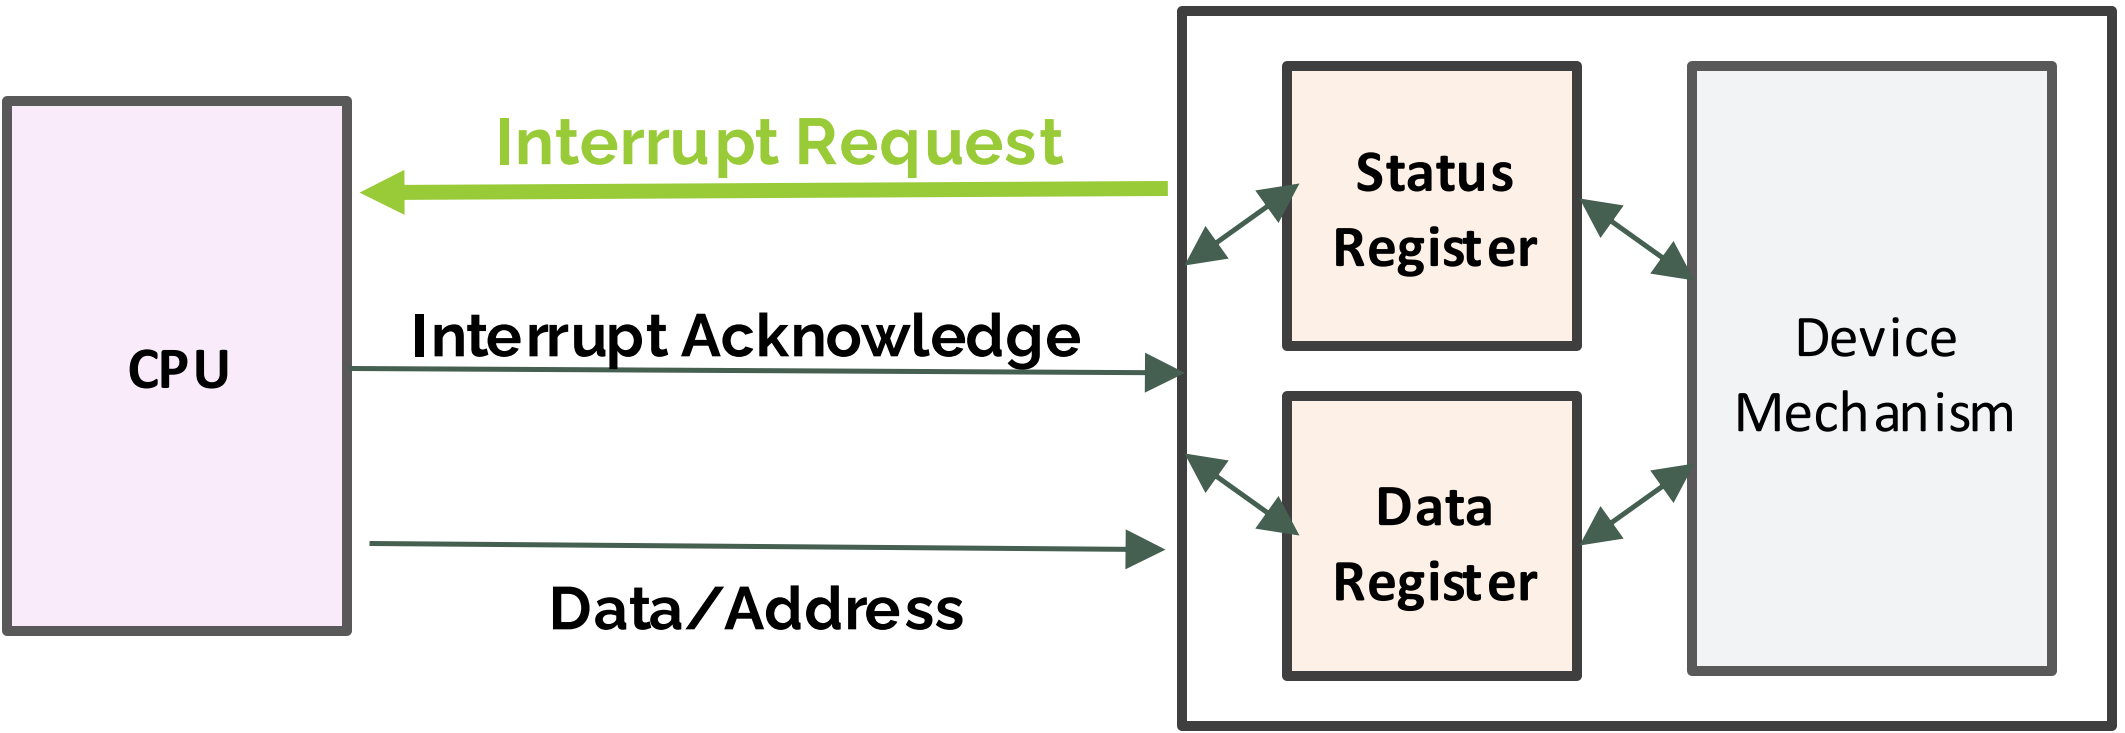
\includegraphics[width=0.65\linewidth]{img/image43.png}
\end{figure}

An interrupt works with the following steps (high-level overview):

\begin{enumerate}
    \item the I/O device decides when to interrupt, like when its status register goes into the ready state
    \item the I/O device wants service from the CPU, so it sends an interrupt request signal
    \item the CPU checks the interrupt request (IRQ) line at every instruction
    \item the CPU is ready to handle the I/O device's request, so it sends an interrupt acknowledge signal
    \item the CPU saves the current value of the program counter
    \item the CPU then changes the program counter to point to the device's interrupt handler
    \item the starting addresses of the interrupt handlers are stored in a table called Interrupt Vector Table/Interrupt Handler Table stored in the CPU's memory
    \item after execution, the interrupt handler executes a special instruction called IRET or RETI to signal it finished execution
    \item the CPU then switches back to the previous program counter to resume its normal execution
\end{enumerate}

\subsection{Priorities and Vectors}

As most systems have more than I/O device, multiple devices can interrupt even at the same time. In this
case, the interrupts are ran in order of priority via a \textbf{Programmable Interrupt Controller} (\textbf{PIC}).

\begin{figure}[H]
    \centering
    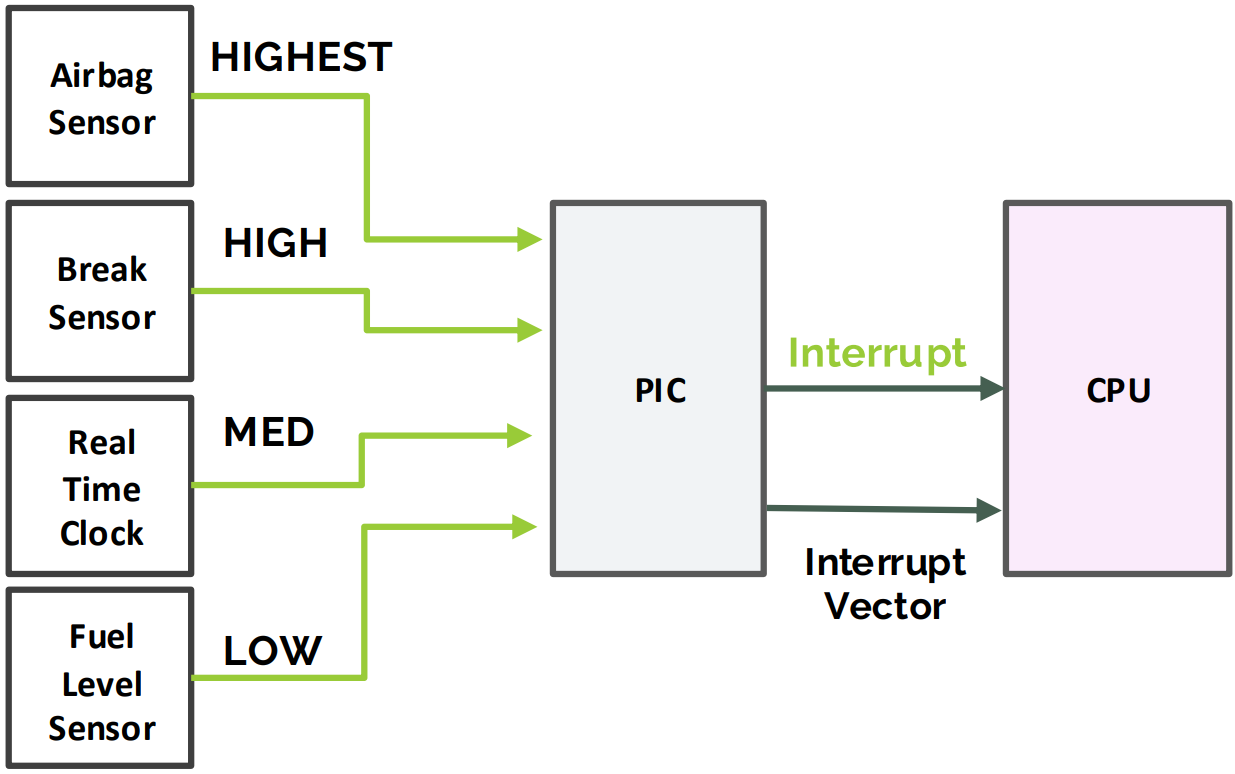
\includegraphics[width=0.65\linewidth]{img/image46.png}
\end{figure}

In the ARM architecture it is called the \textbf{Nested Vector Interrupt Controller} (\textbf{NVIC}). Also it is the interrupt device that specifies its interrupt handler (the index in the Interrupt Vector Table).

\begin{figure}[H]
    \centering
    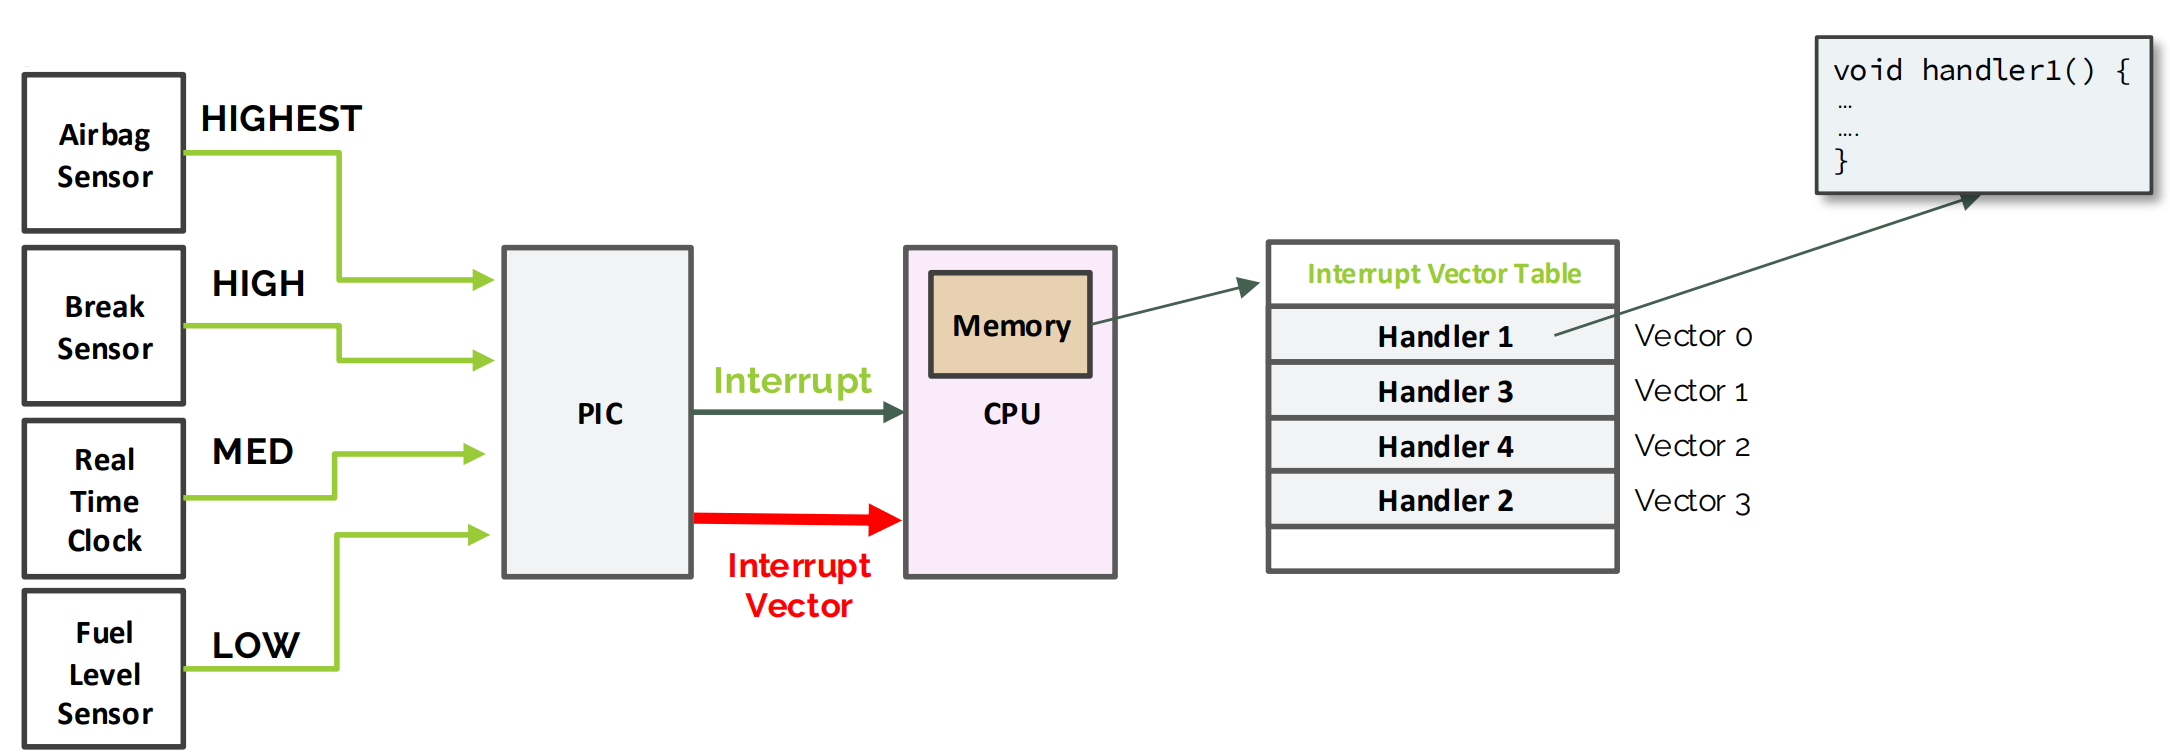
\includegraphics[width=1\linewidth]{img/image44.png}
\end{figure}

\begin{figure}[H]
    \centering
    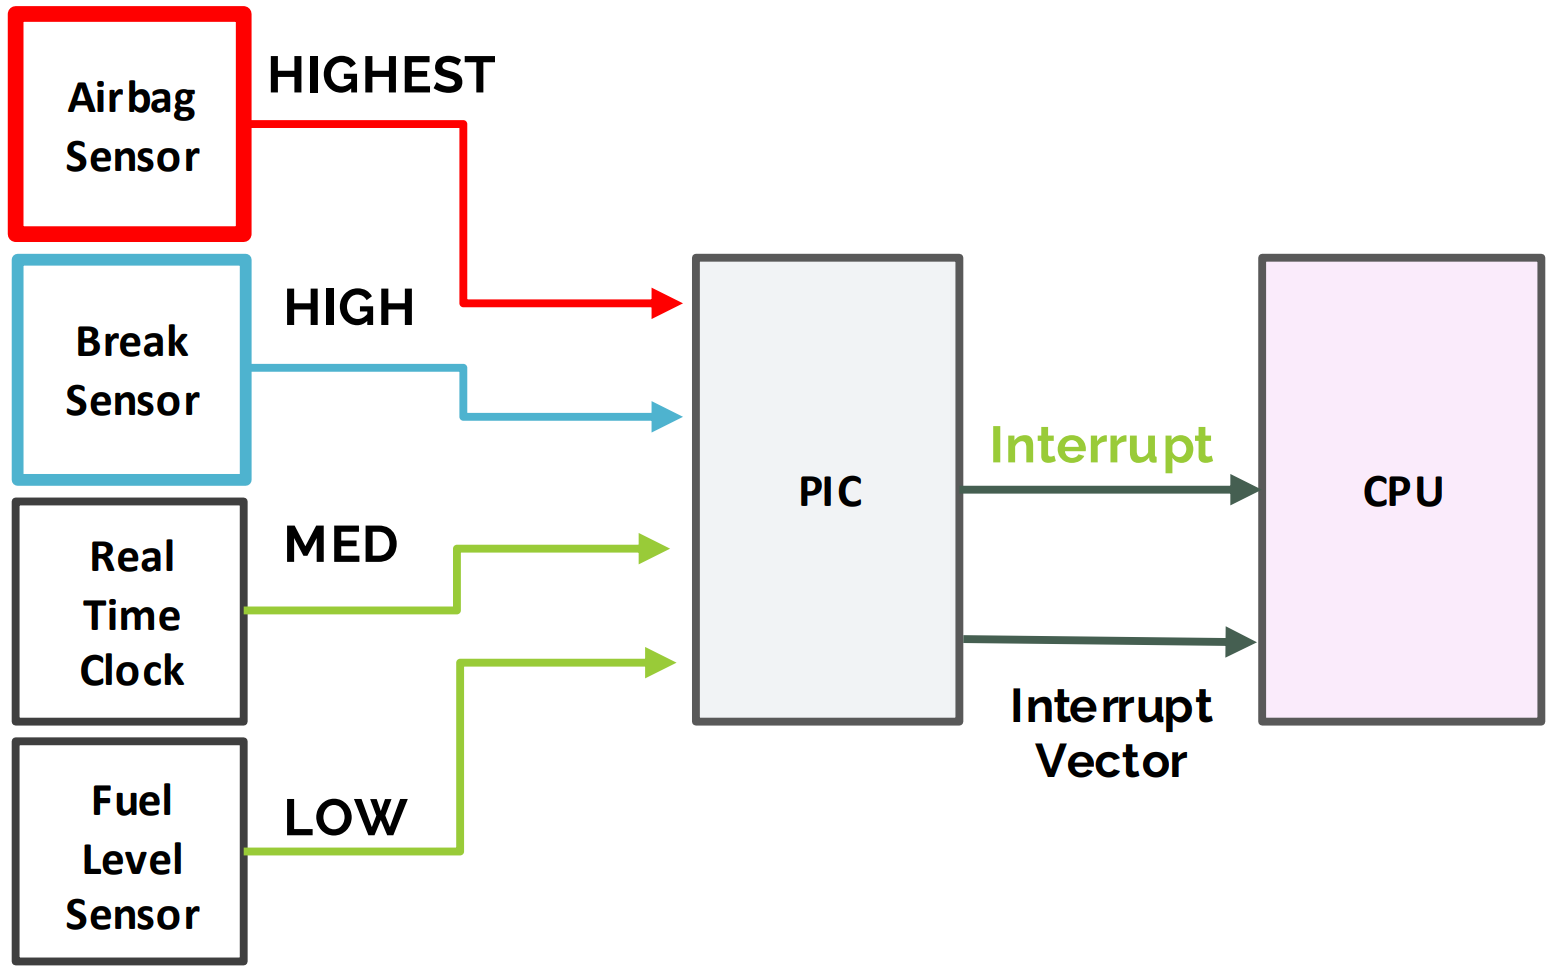
\includegraphics[width=0.65\linewidth]{img/image47.png}
\end{figure}


\paragraph{}
The interrupt devices are connected to the PIC, which tells them if their interrupt handlers are being
executed or are in line through interrupt acknowledge lines. If they are in line, they will also know their
own number of priority.

\begin{figure}[H]
    \centering
    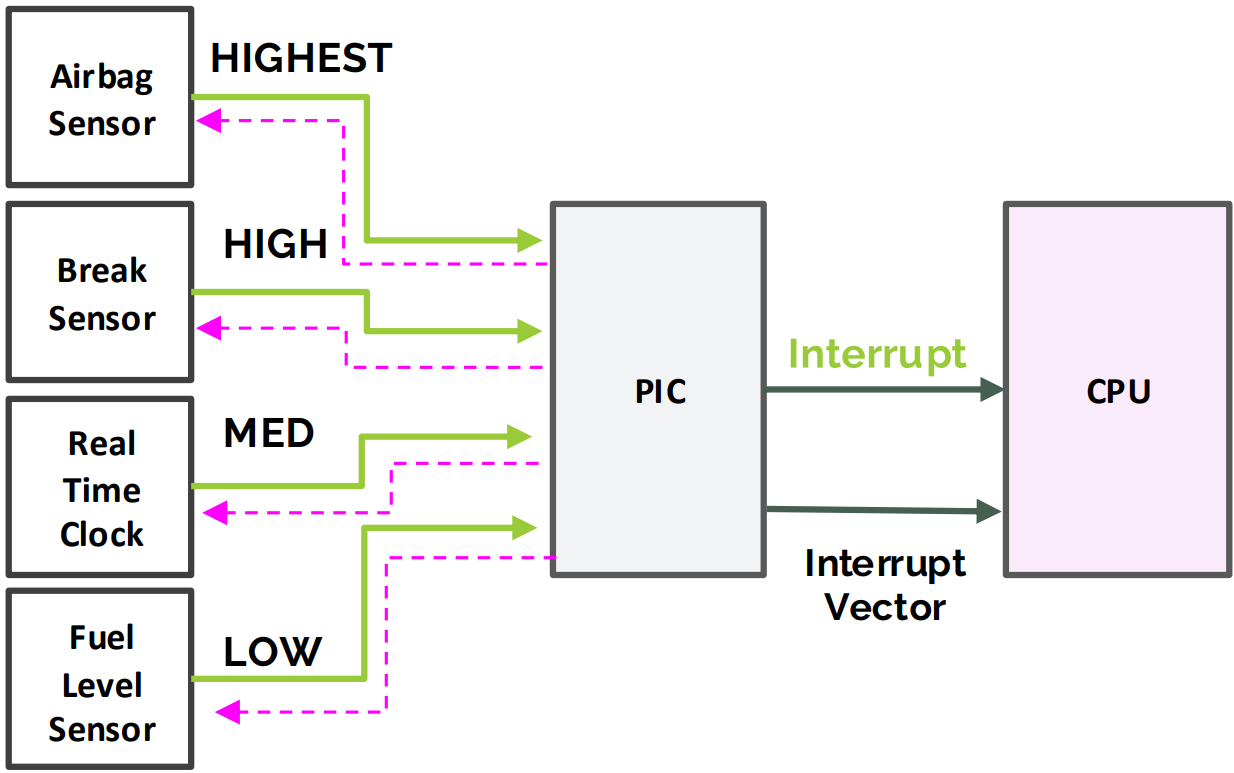
\includegraphics[width=0.65\linewidth]{img/image48.png}
\end{figure}

Nested interrupts must be prevented (ISR being ran while another ISR is being ran already).

\paragraph{NOTE: } Interrupt handler = ISR = Interrupt Service Routine


\begin{figure}[H]
    \centering
    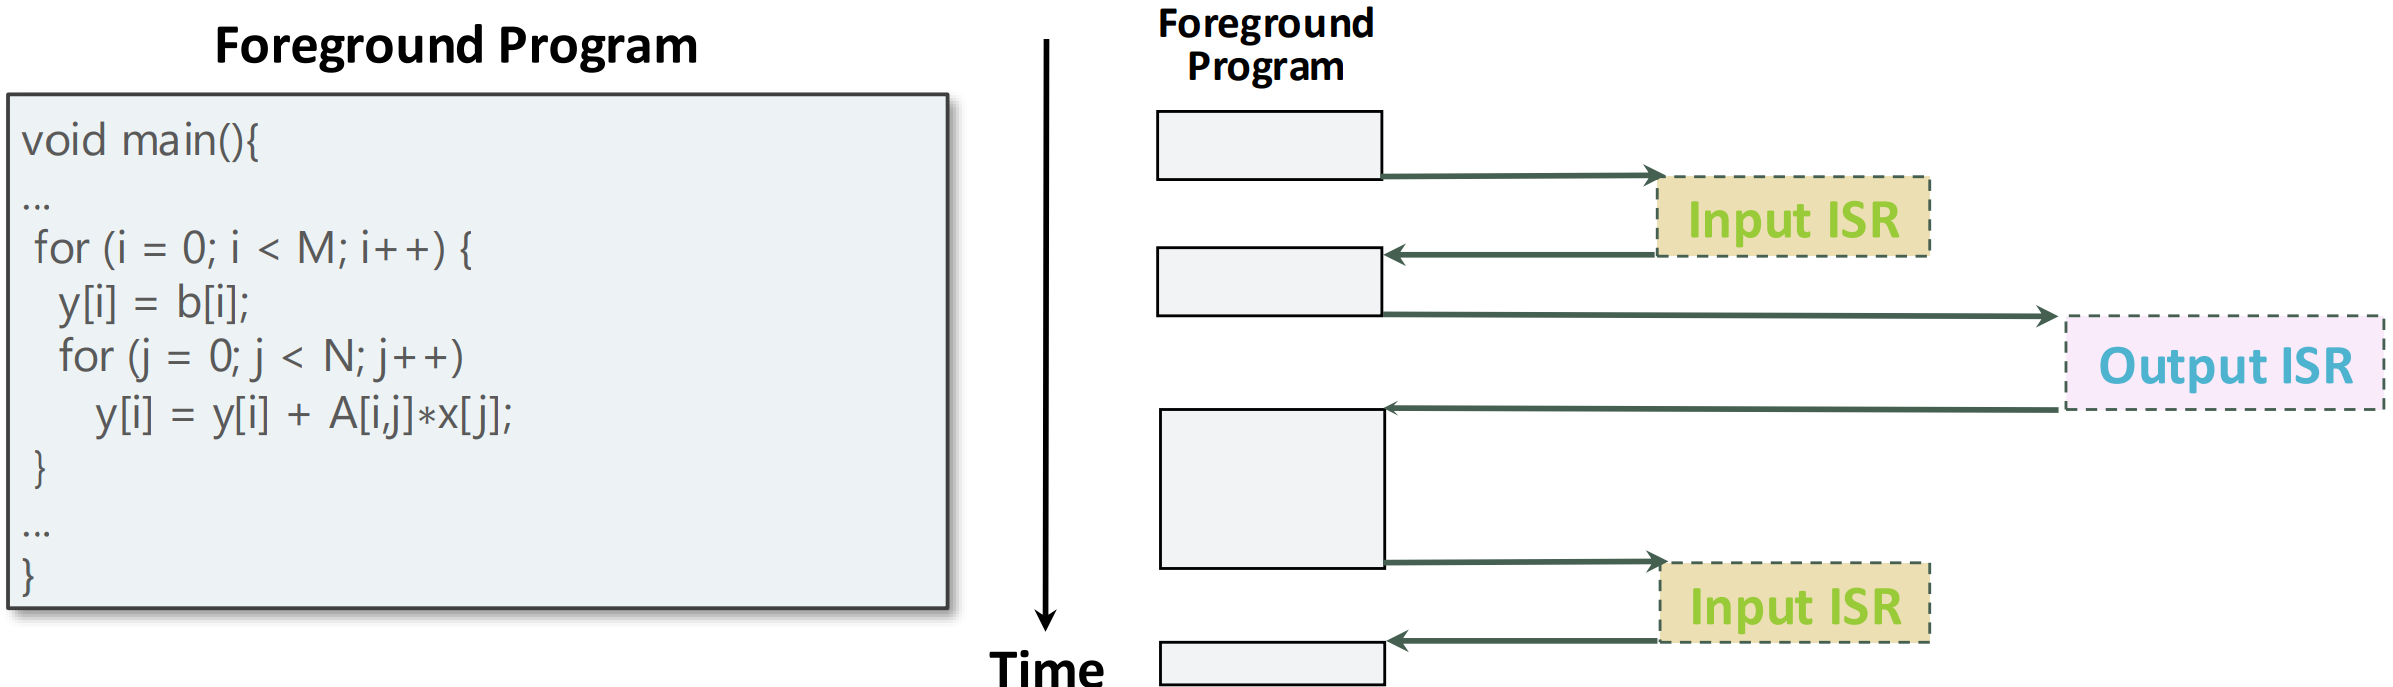
\includegraphics[width=0.9\linewidth]{img/image42.png}
\end{figure}


\section{Interrupt Masking}

Interrupt masking is a technique used to control and prioritize interrupt handling. It is typically used
to ensure that high-priority interrupts are handled promptly, especially in real-time and safety-critical
systems where specific interrupts must be handled immediately to meet timing or safety requirements.

\paragraph{"Masking"} means temporarily disabling an interrupt. This means that as soon as the CPU
acknowledges a higher priority interrupt, it immediately pauses the current ISR, executes the higher
priority interrupt's ISR before resuming the previous one.

The \textbf{PIC} is used to facilitate interrupt masking, via registers or configuration settings to enable or disable
specific interrupt sources.


\section{Non-Maskable Interrupt}

Non-maskable interrupt (NMI) is an interrupt that cannot be masked so it will be executed 100% instantly
without getting turned off. It is usually reserved for interrupts caused by power failures to save critical
state in nonvolatile memory, turn off I/O devices...

NMIs are device specific.



\section{Interrupt vs Exceptions}

While \textbf{both do the same thing} (interrupt the current flow of the program), interrupt is meant when it's done
by a \textbf{hardware device}, while an exception is done by the \textbf{software}.

\subsection{Example \#1: interrupt}


The following example showcases the same program from the previous example, now using interrupts:

\begin{lstlisting}[language=c]

    /* get a character and put in global (called when IN_STATUS is 1) */
     
    void input_handler() {
        achar = read(IN_DATA); /* get character */
        gotchar = TRUE; /* signal to main program */
        write(IN_STATUS,0); /* reset status to initiate next transfer */
    }
    
    /* react to character being sent (called when OUT_STATUS is 0) */
    void output_handler() {
        /* don't have to do anything */
    }
\end{lstlisting}

The \verb|input_handler| function does the following:

\begin{itemize}
    \item[-] stores the new character, taken from the input device's data register, into achar
    \item[-] turns gotchar to true to signal to the main program that there's a new character
    \item[-] resets the input device's status register to 0, ready state
\end{itemize}


All input device operations are done in the interrupt handler.


\subsubsection{Mainprogram:}

\begin{lstlisting}[language=c]

    main() {
        while (TRUE) { /* read then write forever */
            if (gotchar){ /* write a character */
                write(OUT_DATA,achar); /* put character in device */
                write(OUT_STATUS,1); /* set status to initiate write */
                gotchar = FALSE; /* reset flag */
            }
        }
    }
\end{lstlisting}

\begin{enumerate}
    \item The gotchar variable is checked if true
    \item Once it is, the character is written in the output device's data register and the output device's status register is set to 1, signaling it to initiate write
    \item Then resets the gotchar variable to false as it waits for a new character
\end{enumerate}

A few issues in this example:

\begin{itemize}
    \item[] output device is not waited for when it finishes writing
    \item[] character can be overwritten before it is written in the output device's data register
\end{itemize}

\textit{This example is used to just show off how interrupts work.}


\subsection{Example \#2: Interrupt}

The following example showcases the previous program but more sophisticated and improved thanks to
the use of a \textbf{wraparound/circular buffer} (data structure) to hold the new characters, which also fixes the
issues of the previous example.


\begin{figure}[H]
    \centering
    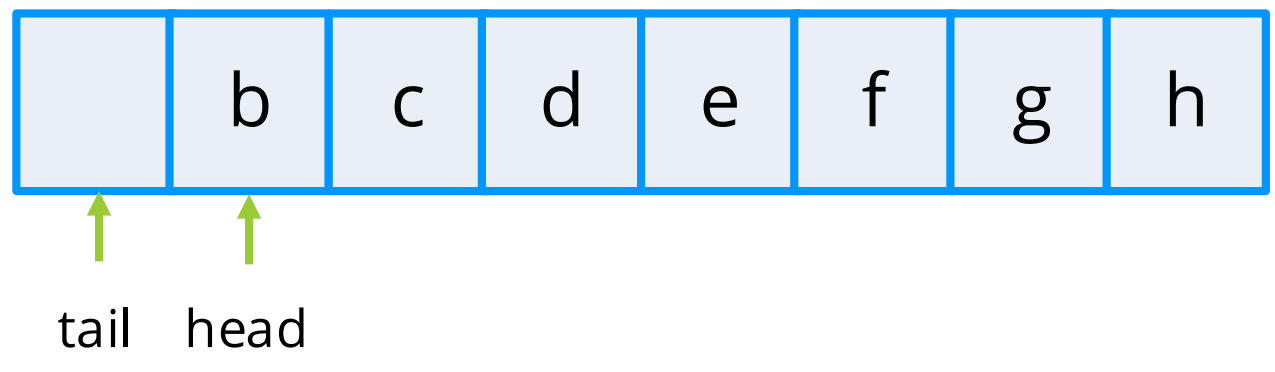
\includegraphics[width=0.6\linewidth]{img/image45.png}
\end{figure}

\subsubsection{Here's an implementation of the circular buffer:}

\begin{lstlisting}

    #define BUF_SIZE 8
    char io_buf[BUF_SIZE]; /* character buffer */
    int buf_head = 0, buf_tail = 0; /* current position in buffer */
    int error = 0; /* set to 1 if buffer ever overflows */
    
    int empty_buffer() { /* returns TRUE if buffer is empty */
        return buf_head == buf_tail;
    }
    
    int full_buffer() { /* returns TRUE if buffer is full */
        return (buf_tail+1) % BUF_SIZE == buf_head ;
    }
    
    int nchars() { /* returns the number of characters in the buffer */
        if (buf_head >= buf_tail)
            return buf_head - buf_tail;
        else
            return BUF_SIZE - buf_tail - buf_head;
    }
    
    void add_char(char achar) { /* add a character to the buffer head */
        io_buf[buf_tail++] = achar;
        /* check pointer */
        if (buf_tail == BUF_SIZE)
        buf_tail = 0;
    }
    char remove_char() { /* take a character from the buffer head */
        char achar;
        achar = io_buf[buf_head++];
        /* check pointer */
        if (buf_head == BUF_SIZE)
            buf_head = 0;
        return achar;
    }
\end{lstlisting}

Here are the new input/output handlers, making use of the circular buffer:

\begin{lstlisting}

    #define IN_DATA 0x1000
    #define IN_STATUS 0x1001
    
    /* get a character (called when IN_STATUS is 1) */
    void input_handler() {
        char achar;
        
        if (full_buffer()) /* error */
            error = 1;
        else { /* read the character and update pointer */
            achar = read(IN_DATA); /* read character */
            add_char(achar); /* add to queue */
        }    
        write(IN_STATUS,0); /* set status register back to 0 */
        
        /* if buffer was empty, start a new output transaction */
        if (nchars() == 1) { /* buffer had been empty until this interrupt */
            write(OUT_DATA,remove_char()); /* send character */
            write(OUT_STATUS,1); /* turn device on */
        }
    }
\end{lstlisting}

\begin{lstlisting}

    #define OUT_DATA 0x1100
    #define OUT_STATUS 0x1101
    
    /* react to character being sent (called when OUT_STATUS is 0) */
    void output_handler() {
        if (!empty_buffer()) { /* start a new character */
            write(OUT_DATA,remove_char());/* send character */
            write(OUT_STATUS,1); /* turn device on */
        }
    }
\end{lstlisting}

The input handler writes the data to the output device when the buffer is empty.

When the buffer is not empty, the output handler keeps writing data to the output device while emptying
the buffer.

\subsection{Cons of Interrupts}

\begin{itemize}
    \item Interrupts increase the program's complexity
    \item Finding bugs is difficult because interrupts are triggered by hardware devices
    \item Concurrency with interrupt handlers can cause bugs if they don't save/restore CPU registers that they modify during executions, causing variables in the foreground program to change mysteriously
\end{itemize}

\section{Overhead of Interrupts}

An interrupt causes a change in the program counter, which incurs a branch penalty: the pipeline of
instructions gets invalidated. So if interrupts occur frequently there will be a noticeable overhead.


If the interrupt automatically stores CPU registers, it requires extra cycles.


Also the acknowledgements, priorities, and the obtaining the index in the table from the device all require
extra cycles.

\paragraph{}
All around interrupts add overhead and latency to the device.
Real-time, or time-critical applications require great knowledge of interrupt and its mechanisms as to
minimise overhead.

\begin{figure}[H]
    \centering
    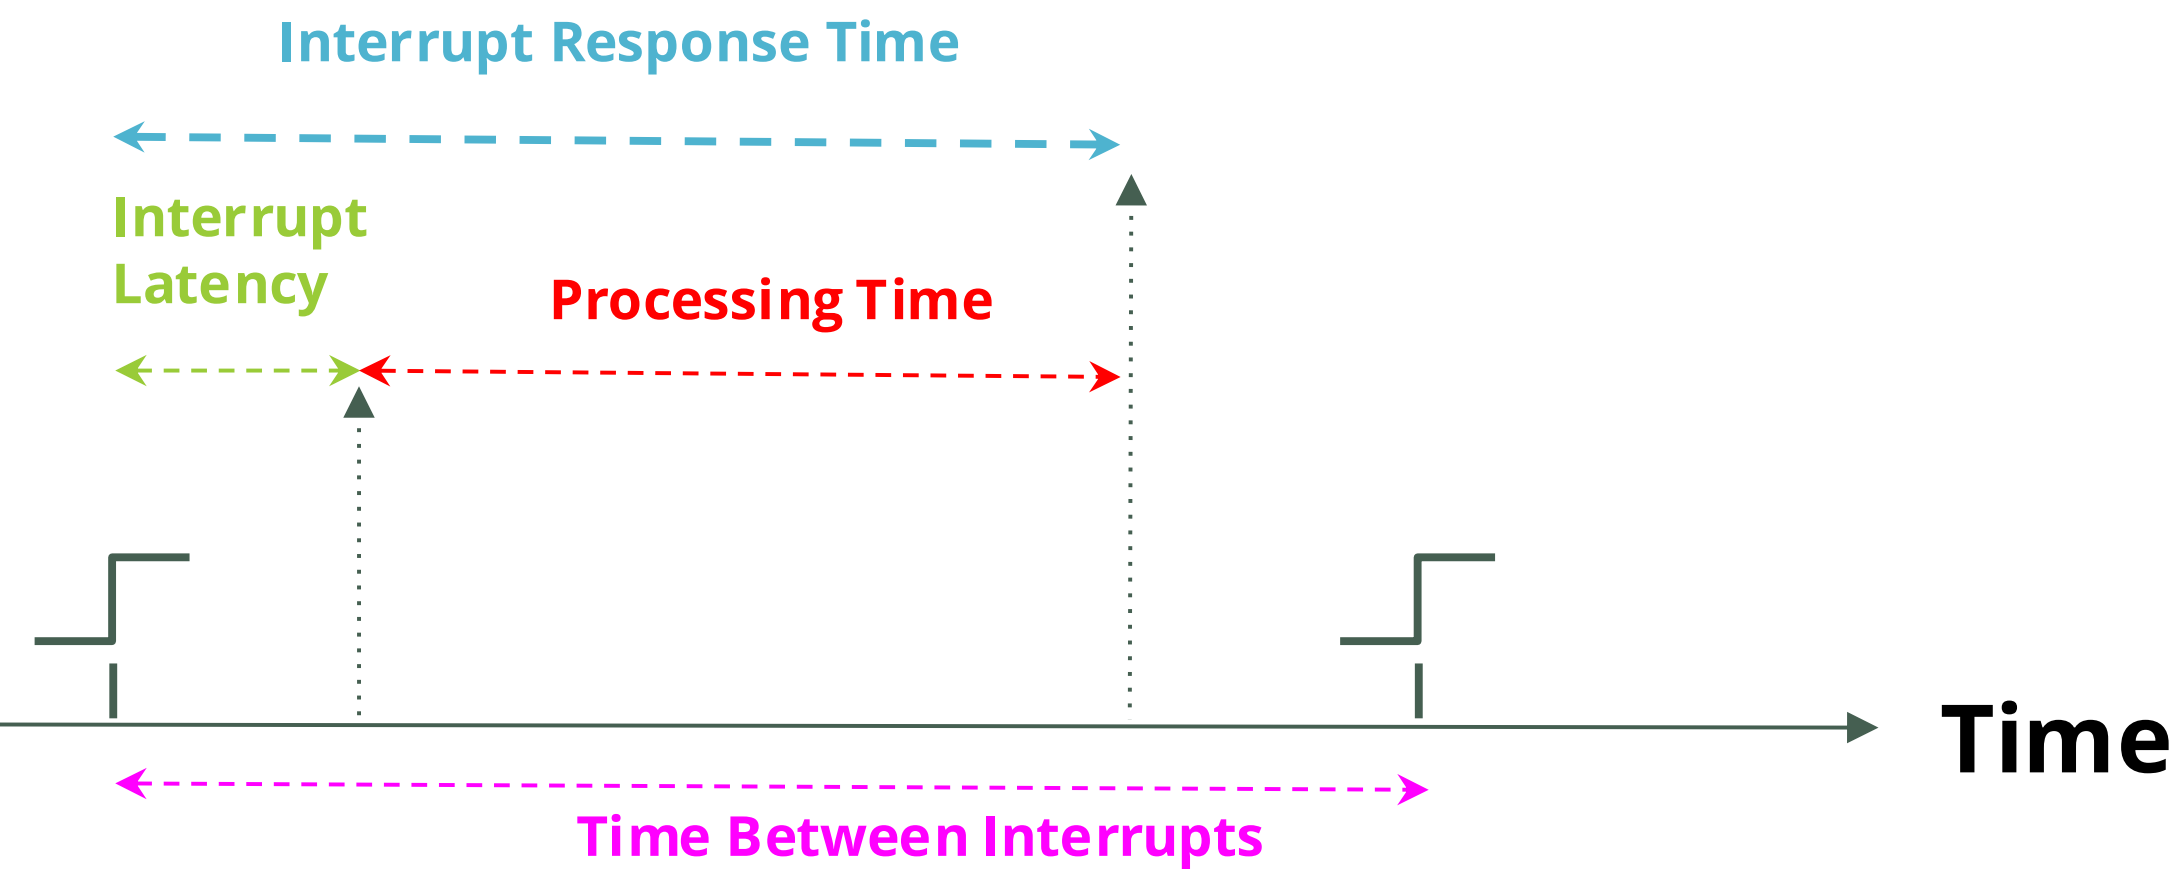
\includegraphics[width=0.85\linewidth]{img/image49.png}
\end{figure}

\section{Co-processors}

They are processors attached to the CPU that implement some instructions, mostly maths instructions. The
most common co-processor adds \textbf{floating-point arithmetic capabilities}.

A co-processor has its own registers and hardware. The co-processor is ordered by the CPU to activate, receive the instruction and execute it when it receives
a co-processor instruction via certain opcodes reserved in the instruction set.


The CPU can either:

\begin{itemize}
    \item suspend execution to wait for the co-processor to finish
    \item continue executing instructions (super-scalar approach)
\end{itemize}
\chapter{Introduction to TI MSP432 Launchpad}

\section{Embedded System Development Platform}

It consists of the \textbf{host system}, that has the cross compiler, linker and source-level debugger.
It also consists of the \textbf{target system}, with debugger, processor, sensors...


There must be connections between the host and target system to \textbf{download program images and
transmit debugger information} between the host debugger and the target debug agent.

\begin{figure}[H]
    \centering
    \includegraphics[width=0.8\linewidth]{img/image50.png}
\end{figure}

In the \textit{TI MSP432 Launchpad} the Programmer \& debugger is also inside the target system.

\subsection{Launchpad}
It's a whole Printed Circuit Board (PCB) used as a development kit, allowing you to mess around with the
code and re-flash it each time. When the code is ready for production, and can be burned in a ROM, all
you will need is the processor. Most vendors provide these kits.
\begin{figure}[H]
    \centering
    \includegraphics[width=0.7\linewidth]{img/image51.png}
\end{figure}

\section{Microcontroller Components}



\begin{figure}[H]
    \centering
    \includegraphics[width=1\linewidth]{img/MSP432P401M-functional-block-diagram.png}
\end{figure}

\begin{figure}[H]
    \centering
    \includegraphics[width=1\linewidth]{img/image53.png}
\end{figure}

\newpage
\subsection{TI-MSP432 microcontroller main features}

\begin{itemize}
    \item[-] \textbf{ARM(r) Cortex(tm)-M4F} processor - Designed for low-power, embedded systems application
    \item[-] MSP stands for Mixed Signals Processing, can read both analogue and digital values
    \item[-] 100-pin microcontroller chip
    \item[-] Peripherals: 256KB on-chip Flash memory for code, 64KB on-chip SRAM for data, large number of on-chip peripherals
\end{itemize}


\subsection{Memory Map in MSP432P401R}

\begin{figure}[H]
    \centering
    \includegraphics[width=0.6\linewidth]{img/image54.png}
\end{figure}

\section{Running an application on the launchpad}

\textbf{New project:}
    \begin{itemize}
        \item[$\rightarrow$] Create new project
        \item[$\rightarrow$] Select target microcontroller
        \item[$\rightarrow$] Empty project with main.c
        \item[$\rightarrow$] Everything else default
    \end{itemize}
\textbf{Compiling the project:}
    \begin{itemize}
        \item[$\rightarrow$] Rebuild the project
    \end{itemize}
\textbf{Burn/Load the project onto the launchpad:}
\begin{itemize}
        \item[$\rightarrow$] Debug project
    \end{itemize}

    The application runs on bare metal programming, thus there is no OS or external support whatsoever.
You can see all instructions and manipulate memory at will. All you're facing is the actual hardware. We
can see the registers, variables, memory browser, assembly instructions and so on (expressions,
breakpoints...).

\section{Peripherals}


They are external to CPU:

\begin{minipage}{\linewidth}
      \centering
      \begin{minipage}{0.40\linewidth}
            \begin{itemize}
                \item Memory-mapped I/O to configure peripherals
                \item Pointers
                \item Memory Reads/Writes
                \item Use of Bit Manipulation
            \end{itemize}
      \end{minipage}
      \hspace{0.05\linewidth}
      \begin{minipage}{0.35\linewidth}
            \begin{figure}[H]
                \centering
                \includegraphics[width=1\linewidth]{img/image55.png}
            \end{figure}
      \end{minipage}
  \end{minipage}








\section{GPIO - Input/Output Systems}

\textbf{GPIO-General Purpose IO}: Pin – physical connection to microcontroller, Port – combination of pins
\textbf{Input/Output}: method to get data in/out of microcontroller

\begin{figure}[H]
    \centering
    \includegraphics[width=0.5\linewidth]{img/image56.png}
\end{figure}

Pins may have different features, to enable an alternative function, set up the appropriate register

\begin{figure}[H]
    \centering
    \includegraphics[width=0.5\linewidth]{img/image57.png}
\end{figure}

In the microcontroller, we have two types of I/O:

\begin{itemize}
    \item[] \textbf{General Purpose I/O} (GPIO) - the GPIO ports are used for interfacing devices such as LEDs, switches, LCD, keypad, and so on.
    \item[] \textbf{Special purpose I/O} - These I/O ports have designated function such as ADC (Analog-toDigital), Timer, UART (universal asynchronous receiver transmitter), and so on.
\end{itemize}

The GPIO ports in MSP432 are designated as port P1 to P10 - Simple I/O or Digital I/O ports - and PJ - special function such as crystal oscillator and JTAG connections.

\newpage
\section{Configuring LED}

To \textbf{configure} LED on P1.0

\begin{itemize}
    \item set direction to output: \textbf{P1DIR}
    \item Set P1.0 output to high: \textbf{P1OUT}
\end{itemize}


\begin{figure}[H]
    \centering
    \includegraphics[width=0.7\linewidth]{img/image60.png}
\end{figure}

To\textbf{ turn on} LED, P1.0\_LED1: voltage needs to be a Logical HI (VCC 3.3V).

Also Required to Set Pin to \textbf{I/O Mode} (P1SELx).

\paragraph{Two important registers:} IO Direction Register, \textbf{P1DIR}, IO Output Register, \textbf{P1OUT}.

\subsection{P1DIR Register}

Port Direction Register sets the
pin to:

\begin{itemize}
    \item 0: an input
    \item 1: an output
\end{itemize}

\begin{lstlisting}[language=c++]

    /* Configure P1.0 output */
    P1->DIR |= BIT0; 
\end{lstlisting}


\subsection{P1OUT Register}

Port Output Register sets output to:

\begin{itemize}
    \item 0: Output set to LOW (GND)
    \item 1: Output set to HIGH (VCC)
\end{itemize}

\begin{lstlisting}[language=c++]

    /* Configure P1.0 output */
    P1->DIR |= BIT0;
    /* Set P1.0 HIGH */
    P1->OUT |= BIT0;
\end{lstlisting}

\section{Configure the buttons}

Buttons are connected to P1.1 and P1.34

\begin{lstlisting}[language=c++]

    /* Configure P1.1 as input*/
    P1->DIR = ~BIT1; //BIT0 as output
    /* Select pullup*/
    P1->OUT = BIT1; //BIT0 pulldown
    /* Enable pullup*/
    P1->REN = BIT1; //BIT0 disable
    /* Set as I/O */
    P1->SEL0 = 0;   //general purpose I/O selected
    P1->SEL1 = 0;
    ...
    /* Catch Button Press */
    while (P1->IN & BIT1);
    while (!(P1->IN & BIT1));
    ...
\end{lstlisting}

\subsection{Pull-up and Pull-down Resistors}

If we do not use internal pull-up (or pull-down) resistors, we have a
problem. We need to ensure a known value on the output if a pin is left floating.

We want the switch SW to pull the pin to ground, so we enable the pull-up. The pin value is:

\begin{itemize}
    \item High when SW is not pressed
    \item Low when SW is pressed
\end{itemize}


\begin{figure}[H]
    \centering
    \includegraphics[width=0.5\linewidth]{img/image61.png}
\end{figure}

\chapter{Fundamental Building Blocks}
Embedded software must run at a required rate to meet system deadlines, must meet power consumption
requirements, must meet timing requirements and must fit into the allowed amount of memory.


Given these constraints, everything is mostly done from scratch and it's hard to find perfect libraries for
our applications.


Despite this, there are basic building blocks that can compose a program.

\section{Finite State Machines - FSMs}

An FSM is simply a machine that reacts to inputs via states.

\begin{figure}[H]
    \centering
    \includegraphics[width=0.5\linewidth]{img/image_60.png}
    \caption{Simple example of FSM}
\end{figure}

We can model it using this Pseudo-Code:


\begin{lstlisting}[language=c++]

    #define IDLE 0
    #define SEATED 1
    #define BELTED 2
    #define BUZZER 3
    
    switch(state) { /* check the current state */
    
        case IDLE:
             if (seat){ state = SEATED; timer_on = TRUE; }
             /* default case is self-loop */
             break;
        case SEATED:
             if (belt) state = BELTED; /* won't hear the buzzer */
             else if (timer) state = BUZZER; /* did not put on belt in time */
             /* default case is self-loop */
             break;
        case BELTED:
             if (!seat) state = IDLE; /* person left */
             else if (!belt) state = SEATED; /* person still in seat */
             break;
        case BUZZER:
             if (belt) state = BELTED; /* belt is on---turn off buzzer */
             else if (!seat) state = IDLE; /* no one in seat-turn off buzzer */
             break;
    }
\end{lstlisting}


\paragraph{NOTE:} Using function pointers decreases the complexity of the FSM program.


\begin{figure}[H]
    \centering
    \includegraphics[width=0.6\linewidth]{img/image_61.png}
\end{figure}

\subsection{Define states and and state machine structure:}
\begin{lstlisting}[language=c++]

    typedef enum{
        STATE_A;
        STATE_B;
        STATE_C;
        STATE_D;
        NUM_STATES
    }State_t;
    
    typedef struct{
        State_t state; /* defines the command */
        void (*func)(void); /* defines the function to execute */
    } StateMachine_t;
\end{lstlisting}



\subsection{Declare functions that implement states, variable to hold current state and the state machine itself:}

\begin{lstlisting}[language=c++]

    /* state machine function prototypes */
    void fn_StateA(void);
    void fn_StateB(void);
    void fn_StateC(void);
    void fn_StateD(void);
    
    /* variable that holds the current state */
    State_t cur_state = STATE_A:
    
    StateMachine_t StateMachine[] = {
        {STATE_A, fn_StateA},
        {STATE_B, fn_StateB},
        {STATE_C, fn_StateC},
        {STATE_D, fn_StateD}
    } ;
\end{lstlisting}

\newpage

\subsection{Fill the functions:}

\begin{lstlisting}[language=c++]

    void fn_StateA(void){
        /* add the necessary code here */
        cur_state = STATE_B;
    }
    void fn_StateB(void){
        /* add the necessary code here */
        cur_state = STATE_C;
    }
    void fn_StateC(void){
        /* add the necessary code here */
        cur_state = STATE_D;
    }
    void fn_StateD(void){
        /* add the necessary code here */
        cur_state = STATE_A;
    }
\end{lstlisting}



\subsection{Run function:}
\begin{lstlisting}[language=c++]

    void run(void){    
        if(cur_state < NUM_STATES){
            (*StateMachine[cur_state].func)();
        }else{
            // error
        }
    }
\end{lstlisting}

\section{Circular Buffer}

Circular buffers are a data structure useful for stream-oriented processing (where data comes regularly
and must be processed on the fly, basically we can read values but also must consume values).

\section{Queue}

Queues are a data structure useful for data that arrives and departs at unpredictable times.
A synonym of queue is \textbf{elastic buffer.}
\paragraph{}
One way to implement a queue is through linked lists, that allows the queue to grow to an arbitrary size at
the cost of overhead of dynamic memory allocation (therefore not recommended).
Another way is through an array to hold all the data.
\paragraph{}
A queue may have varying numbers of elements in it as it doesn't have to accommodate all of the incoming
data, but a circular buffer will always have a fixed number of data.


\section{Producer/Consumer problems}

Some aspects of an application can be a producer and others can be a consumer. This is meant in
regards to writing (producing) and reading (consuming) data. Basically we should strive to keep the loads
balanced

\section{Pragma}

A \verb|pragma| is a compiler directive, usually platform-specific.

\begin{figure}[H]
    \centering
    \includegraphics[width=0.75\linewidth]{img/image_62.png}
\end{figure}
In this case, it is used to specify the data section of interruptVectors in .intvects
interruptVectors is the Interrupt Vector Table.

\paragraph{}
Since it is a constant array it will be placed in the Flash memory.
The first entry is the Initial Stack Pointer to initialised the Core CPU registers.

The other five entries are High-Priority ARM Core Exceptions.
The rest of the handlers are for GPIO interrupts


\section{Default Handler}

\begin{lstlisting}[language=c++]

    ...
    /* Forward declaration of the default fault handlers. */
    void Default_Handler (void) __attribute__((weak));
    ...
    /* This is the code that gets called when the processor receives an unexpected */
    /* interrupt. This simply enters an infinite loop, preserving the system state */
    /* for examination by a debugger. */
    
    void Default_Handler(void){
    
        /* Fault trap exempt from ULP advisor */
        #pragma diag_push
        #pragma CHECK_ULP("-2.1")
        
        /* Enter an infinite loop. */
        while(1){
        
        }
        
        #pragma diag_pop
    }
\end{lstlisting}


\verb|__attribute__((weak))| means that it can be overridden by the developer

\subsection{Overriding Default Handlers}

\begin{lstlisting}[language=c++]

    ...
    extern void PORT1_IRQHandler (void) __attribute__((weak,alias("Default_Handler")));
    extern void PORT2_IRQHandler (void) __attribute__((weak,alias("Default_Handler")));
    extern void PORT3_IRQHandler (void) __attribute__((weak,alias("Default_Handler")));
    extern void PORT4_IRQHandler (void) __attribute__((weak,alias("Default_Handler")));
    extern void PORT5_IRQHandler (void) __attribute__((weak,alias("Default_Handler")));
    extern void PORT6_IRQHandler (void) __attribute__((weak,alias("Default_Handler")));
    ...
\end{lstlisting}

\textit{alias} means that it defaults to \verb|Default_Handler| if it is not implemented.
\textit{extern} means that the function can be defined in other source files.


\section{Implementing Interrupts}

We can do this by using Interrupt \textbf{Edge Select Registers} (PxIES), \textbf{Interrupt Flag Registers} (PxIFG),
and \textbf{Interrupt Enable Registers} (PxIE).

\paragraph{Example: } left button P1.1
\begin{lstlisting}[language=c++]

    P1->IES = BIT1; //PxIFG flag set with high-to-low-transition, BITO viceversa
    P1->IE = BIT1;  //Port interrupt enabled, BIT0 viceversa
    P1->IFG = 0;    //No interrupt is pending/Clear all interrupt flags, 1 viceversa
\end{lstlisting}


Now we need to program the NVIC, enabling the corresponding ISR on the NVIC IRQ assignment, by
using NVIC's ISER (Instruction Set Enable Registers):

\begin{itemize}
    \item We know that the IRQ\# (IRQ number) of the I/O Port P1 is 35 from the documentation
    \item We know that the ISER1 register covers all IRQ\# from 32 to 63
\end{itemize}
\begin{lstlisting}[language=c++]

    NVIC->ISER[1] = 1 << ((PORT1_IRQn) & 31);
\end{lstlisting}


The instruction first calculates the bitwise AND ( \& ) between \verb|PORT1_IRQn| and 31, the maximum
index of the \verb|ISER[1]| register.
This is a common safety precaution in embedded software to prevent unintentional modification of
the bits outside the valid range of the register.
After that, the number 1 is then shifted X places to the left, where X is the result of the bitwise AND.

\paragraph{}
This is because the IRQ\# is 35, so we needed to shift it 3 places from 32. 3 was the exact result of the
bitwise AND between the IRQ\# and the number 31.

\paragraph{}
Then we write the actual ISR:


\begin{lstlisting}[language=c++]

    /* Port1 ISR */
    void PORT1_IRQHandler(void){
        // Toggling the output on the LED
        if(P1->IFG & BIT1)
        P1->OUT ^= BIT0;
        // clear the flag
        P1->IFG &= ~BIT1;
    }
\end{lstlisting}

It checks if there's an interrupt; if there is one it toggles the LED's output and then clear the flag (removes
the pending interrupt so we can catch the next one).

\section{Low-Power Modes}

MSP432 supports several power modes for operation: allow for the optimisation of power for a given application scenario

\begin{figure}[H]
    \centering
    \includegraphics[width=0.9\linewidth]{img/image_63.png}
\end{figure}

To enter LPM0 mode, simply use: \verb|__sleep();|
\chapter{Timer Overview }

A hardware timer is a digital counter that:

\begin{itemize}
    \item counts regular events, normally using a fixed frequency clock source
    \item increments or decrements at a fixed frequency
    \item resets itself when reaching zero, or a predefined value
    \item generates an interrupt when reset
\end{itemize}

A software timer is a function block implemented in software:

\begin{itemize}
    \item usually based on a hardware timer, increments/decrements when interrupted
    \item provides lower time precision
    \item can have multiple instances, notably more than hardware timers
\end{itemize}


\section{Timer use-cases}

Timers can be used to:

\begin{itemize}
    \item[] generate periodic events
    \item[] measure time passed to perform some computational tasks
    \item[] generate pulse width modulation
\end{itemize}

\section{Components of a Standard Timer}

A timer is made of multiple components:

\begin{itemize}
    \item \textbf{Clock source/Oscillator}
    \item \textbf{Prescaler}
    \begin{itemize}
        \item[] Takes the clock source as input
        \item[] Divides the input frequency by a predefined value (4, 8, 16...)
        \item[] Outputs the divided frequency to other components
    \end{itemize}
    \item \textbf{Timer Register}
    \begin{itemize}
        \item[] Is incremented or decremented at a fixed frequency, taken from the prescaler
        \item[] Is driven by the output from the prescaler, often referred to as "ticks"
    \end{itemize}
\end{itemize}


\subsection{Prescalers and software performance}

Prescalers significantly improve system performance when there is a need to:

\begin{itemize}
    \item reduce power consumption
    \item count longer time intervals
    \item In real-time systems, the choice of prescalers should be carefully considered as to meet critical timing requirements
\end{itemize}


\section{Timer Operation Modes}

A standard timer typically has three operation modes.

\subsection{Compare Mode}

The compare mode has a compare register.
The compare register is loaded with a value that is periodically compared with the value in the timer
register.

Once the two values are the same an interrupt can be generated (e.g. every 15 seconds).


\begin{figure}[H]
    \centering
    \includegraphics[width=0.75\linewidth]{img/image65.png}
\end{figure}

\subsection{Capture Mode}
The capture mode has a capture register that captures the current value of the timer register upon the
capture of external events. It can also generate an interrupt.

Optionally, the prescaler can be used to divide the frequency of the events.


\begin{figure}[H]
    \centering
    \includegraphics[width=0.75\linewidth]{img/image66.png}
\end{figure}

\subsubsection{Capture/Compare Registers}
Capture/Compare Registers, also known as CCRs, are registers used to configure and control various
timer-related functionalities. They are registers within the timer module.


\subsection{Pulse-width modulation (PWM) Mode}

This mode uses the width of a pulse to modulate an amplitude, which reflects the duty cycle, which
describes the proportion of the 1 state in one pulse period.

The PWM mode is mainly used to control the power supplied to electrical devices (via on-off intervals).

\begin{figure}[H]
    \centering
    \includegraphics[width=0.75\linewidth]{img/image67.png}
\end{figure}

\section{MSP432 Timer A}
In our launchpad are 4 16-bit timers: TA0, TA1, TA2, TA3. Each one has 7 capture/compare registers,
allowing software timers.

There are TAxR registers that can be manipulated. They can be cleared by setting the TACLR bit.

The timer clock can be sourced from: ACLK, SMCLK, or externally from TAxCLK or INCLK. The clocks
are connected to crystal oscillators. The clock source is selected with the TASSEL bits.
\paragraph{}
The selected clock source may be passed directly to the timer, or it can be slowed down by 2, 4, 8 using
ID bits. Or 2, 3, 4, 5, 6, 7, 8 using TAIDEX bits.

\begin{figure}[H]
    \centering
    \includegraphics[width=0.75\linewidth]{img/image68.png}
\end{figure}

\subsection{Up Mode}
In Up Mode the timer repeatedly counts up to the value of the compare register, TAxCCR0.
Once the two values match the TAxCCR0 CCIFG (capture compare register interrupt flag) is set.
We need to enable the interrupt first. We do this via the CCIE bit in the TAxCCTL0 (Capture/Compare
Control Register) register.

\begin{figure}[H]
    \centering
    \includegraphics[width=0.75\linewidth]{img/image69.png}
\end{figure}

\section{Periodic timer interrupt setup}

We first set the CCIE (Capture Compare Interrupt Enable) bit in TA0 CCTL0 register to enable interrupt.
\begin{lstlisting}[language=c++]

    TIMER_A0->CCTL[0] = TIMER_A_CCTLN_CCIE;

\end{lstlisting}

\paragraph{We are using the first capture/compare register of the first timer A.}

Then we set the value for the comparison.

\begin{lstlisting}[language=c++]

    TIMER_A0->CCTL[0] = TIMER_A_CCTLN_CCIE;
    TIMER_A0->CCR[0] = 50000;
    TIMER_A0->CTL = TIMER_A_CTL_SSEL__SMCLK | TIMER_A_CTL_MC__CONTINUOUS;
\end{lstlisting}


In this case the timer will count up to 50000.
We then set the clock source as SMCLK (3 MHz) in continuous mode.
We use the TA0CTL Control Register for this register.

\paragraph{}

We can also use an input divider (Prescaler) for SMCLK to slow down the input clock signal.
By default the SMCLK is 3 MHz, which means 3,000,000 ticks per second.
By dividing by 8, we get 375,000 ticks per second, the equivalent of 7 interrupts per second.

\begin{lstlisting}[language=c++]

    TIMER_A0->CCTL[0] = TIMER_A_CCTLN_CCIE;
    TIMER_A0->CCR[0] = 50000;
    TIMER_A0->CTL = TIMER_A_CTL_SSEL__SMCLK | TIMER_A_CTL_MC__CONTINUOUS | TIMER_A_CTL_ID_3;
    NVIC->ISER[0] = 1 << ((TA0_0_IRQn) & 31);
\end{lstlisting}

We then have to enable the timer IRQ.
There is a specific IRQ line for CCR0 (the first compare register), while all others (TA0CCR1) share the
same IRQ. Weird design choice.
To counter this (pun intended), we just need to check which CCR triggered the interrupt within the ISR to
distinguish between them.


\begin{figure}[H]
    \centering
    \includegraphics[width=0.6\linewidth]{img/image70.png}
\end{figure}


We then override the Timer Interrupt Handler:
\begin{lstlisting}[language=c++]

    // will be called when TA0CCR0 CCIFG is set
        void TA0_0_IRQHandler(){
        // clear the interrupt flag
        TIMER_A0->CCTL[0] &= ~TIMER_A_CCTLN_CCIFG;
        // toggle LED
        P1->OUT ^= BIT0;
    }
\end{lstlisting}

Just like the other interrupts, we clear the interrupt flag and then do our thing.

\section{Timer Overflow and Counters}
We have to keep in mind timer overflow and counters.

Timer overflows can be used with counters to measure time (e.g. count 1 second if the timer overflows 6
times).

Timer overflows happen because Time Registers have a finite count range (in MSP432 they are 32-bit).
Counters can also be used to measure performance, frequencies, duty cycles and other performance-related metrics.


\section{Watchdog Timer}

Apart from timers we have watchdog timers. Watchdog module performs a controlled system restart after
a software problem occurs/the system gets stuck.
Watchdog timer counts down from a selected interval.
If the selected time interval expires, a system reset is generated.

To edit the control register, the WDTCTL register, we have to insert the password first:


\begin{lstlisting}[language=c++]

    WDT_A->CTL = WDT_A_CTL_PW | WDT_A_CTL_HOLD
\end{lstlisting}

\section{Clocks in MSP432}

Microcontrollers usually have two types of clock resources:

\begin{itemize}
    \item \textbf{on-chip} oscillator (internal oscillator). \textbf{Advantage}: always present
    \item oscillator \textbf{connected} to external crystal (external oscillator). \textbf{Advantage}: higher precision
\end{itemize}

The clock system contains the sources of the various clocks in the device. It also controls the mapping
between the sources and the different clocks in the device.


\subsection{External clock resources:}

\begin{itemize}
    \item LFXTCLK: Low-Frequency Oscillator (LFXT) 32-kHz or below
    \item HFXTCLK: High-Frequency Oscillator (HFXT) 1-MHz to 48-MHz range
\end{itemize}

\subsection{Internal clock resources:}

\begin{itemize}
    \item DCOCLK: Internal Digitally Controlled Oscillator (DCO) Programmable frequencies (3-MHz frequency by default)
    \item VLOCLK: Internal Very-Low-Power Low-Frequency Oscillator (VLO) 9.4-kHz typical frequency
    \item REFOCLK: Internal Low-Power Low-Frequency Oscillator (REFO) Selectable 32.768-kHz or 128-kHz frequencies
    \item MODCLK: Internal Low-Power Oscillator 25-MHz typical frequency
    \item SYSOSC: Internal Oscillator 5-MHz typical frequency
\end{itemize}


\paragraph{Five primary system clock signals are available from the clock module:}

\begin{itemize}
    \item[] ACLK (Auxiliary Clock)
    \item[] MCLK (Master Clock) -> To CPU
    \item[] HSMCLK (Subsystem Master Clock)
    \item[] SMCLK (Low-Speed Subsystem Master Clock)
    \item[] BCLK (Low-Speed Backup Domain Clock)
\end{itemize}

The clock system can be configured or reconfigured by software at any time during program execution.
We have selection and divider signals.


\begin{figure}[H]
    \centering
    \includegraphics[width=0.75\linewidth]{img/image80.png}
\end{figure}

\subsubsection{Example Configuration}

We first need to unlock the CS module for register access, which is protected by password to prevent
inadvertent access.

\begin{lstlisting}[language=c++]

   CS->KEY = CS_KEY_VAL;
    CS->CTL1 |= CS_CTL1_SELA_2 | CS_CTL1_SELS_3 | CS_CTL1_SELM_3
    CS->KEY = 0;
\end{lstlisting}


We could also use a divider to slow down the CPU frequency, by doing this:

\begin{lstlisting}[language=c++]

   CS->KEY = CS_KEY_VAL;
    CS->CTL1 |= CS_CTL1_SELA_2 | CS_CTL1_SELS_3 | CS_CTL1_SELM_3 | CS_CTL1_DIVM_7
    CS->KEY = 0;
\end{lstlisting}


This way we divide the Master Clock signal by $128$.
The DCO by default is $3 MHz$, so it's reduced to $23,437.5 Hz$


\subsection{Slowing CPU to the smallest frequency possible}

We can do this by setting the Master Clock to use the DCO then set the DCO's frequency to 1.5 MHz then
divide it by 128. We achieve $\sim24 kHz$ by doing so.
Or we can set the Master Clock to use VLOCK, which is 9.5 kHz.
\chapter{Software Independence}

A good practice is to write as much software as independent as possible from architectures and platforms
to maximize software \textbf{portability} and \textbf{reusability}.

It's impossible to make everything independent as firmware layers still intersct with hardware and
Assembly code is archiecture dependent as it depends on that hardware's IS.

\begin{figure}[H]
    \centering
    \includegraphics[width=0.75\linewidth]{img/image81.png}
\end{figure}

\section{Binary Interfaces}
The Embedded Application Binary Interface (EABI) is a set of conventions and standards to provide
guidelines for:


\begin{itemize}
    \item how functions are called
    \item how data is organized in memory
    \item how exceptions are handled in embedded applications.
\end{itemize}

Binary interfaces specify details of how the executable must run on this architecture (done by compilers in
most cases).

In architecture terms, an instruction is a fundamental unit of work or operation (arithmetic, logical, program
flow control, load/store), while a word is a fundamental operand size for each operation.

\paragraph{Instruction Sizes:} Instruction size can vary between instruction sets (like ARMv6-M and Thumb-2, for example).
\paragraph{}
Instruction – Fundamental unit of work or operation (Arithmetic, Logical, Program Flow Control, Load/Store)

Word – fundamental operand size for each operation


\paragraph{Standard Integer Sizes: }Variable length types can cause portability issues, we want \textbf{portable data types}. Explicitly defined types that specify storage and design are defined in the \verb|stdint.h| header file.


\begin{lstlisting}[language=c++]

    #ifndef __STDINT_H__
    #define __STDINT_H__
    
    /* 8-bit signed/unsigned Integers */
    typedef signed char int8_t;
    typedef unsigned char uint8_t;
    
    /* 16-bit signed/unsigned Integers */
    typedef signed short int int16_t;
    typedef unsigned short int uint16_t;
    
    /* 32-bit signed/unsigned Integers */
    typedef signed long int int32_t;
    typedef unsigned long int uint32_t;
    
    /* 64-bit signed/unsigned Integers */
    typedef signed long long int int64_t;
    typedef unsigned long long int uint64_t;
    
    #endif /* __STDINT_H__ */
\end{lstlisting}

\section{Pointer Types}

All Pointers are the same length. This because pointer hold addresses in memory of 32-bit.

We need to cast in order to obtain the data inside the memory.

\begin{equation*}
    sizeof(uint8_t*) = sizeof(int16_t*) = sizeof(uint32_t*) = sizeof(float*) = \text{32-Bits!}
\end{equation*}

\begin{lstlisting}[language=c++]

    uint8_t * ptr1 = (uint8_t *) 0x00;
    uint16_t * ptr2 = (uint16_t *) 0x04;
    uint32_t * ptr3 = (uint32_t *) 0x08;
    float * ptr4 = (float *) 0x0C;
\end{lstlisting}

\begin{equation*}
    sizeof(ptr1) = sizeof(ptr2) = sizeof(ptr3) = sizeof(ptr4) = \text{32-Bits!}
\end{equation*}
\begin{equation*}
    sizeof(*ptr1) \ne sizeof(*ptr2)  \ne sizeof(*ptr3)  \ne sizeof(*ptr4)
\end{equation*}

\subsection{NULL Pointers}

In embedded platforms it is always the device (no OS, no other software) that uses pointers carefully.

Null Pointers point to nothing, dereferencing a NULL Pointer can cause an \textbf{exception}.

\section{Data alignment}

\begin{figure}[H]
    \centering
    \includegraphics[width=0.75\linewidth]{img/image82.png}
\end{figure}


\textbf{Load/store data occurs only at aligned addresses in memory.}

\subsection{How to control alignment of data in memory}
We use a compiler attribute which changes based on the compiler.


\begin{lstlisting}[language=c++]

    struct struct_name {
        int8_t var1 int8_t var1 __attribute__ ((aligned(4)));
        int32_t var2;
        int8_t var3;
    } __attribute__ ((packed)); //if not appear default is aligned:  __attribute__ ((aligned));
\end{lstlisting}

In this case, since it's packed, the size of the structure will be 6 bytes rather than 12 bytes when data is
aligned/padded. It will be less efficient for the CPU, however.


\section{Function Attributes}

Compiler attributes can apply to functions.

\verb|inline| is a C99 compiler directive to \verb|inline| a function: rather than calling small functions, since calling
functions adds overhead, functions are automatically added where they are called. The compilers won't
necessarily \verb|inline| every function unless \verb|((always_inline))| (GCC attribute) is used.

Inlining is good for small functions.

\begin{figure}[H]
    \centering
    \includegraphics[width=0.75\linewidth]{img/image83.png}
\end{figure}


\subsection{Function Pragmas}

Pragmas are preprocessor directives that provide special instructions to the compiler via software and not
command line.

\begin{lstlisting}[language=c++]

    #pragma GCC push
    #pragma GCC optimize ("O0")
    int32_t add( int32_t x, int32_t y ){
        return (x + y);
    }
    #pragma GCC pop
\end{lstlisting}

\section{Preprocessor Directives}

\begin{figure}[H]
    \centering
    \includegraphics[width=0.75\linewidth]{img/image84.png}
\end{figure}

Preprocessor directives are special keywords used by the preprocessor before compilation.
All of them start with \# sign:

\begin{itemize}
    \item[--] Important Directives
    \item[--] \#define, \#undef
    \item[--] \#ifndef, \#ifdef, \#endif
    \item[--] \#include
    \item[--] \#warning, \#error
    \item[--] \#pragma
\end{itemize}


\begin{figure}[H]
    \centering
    \includegraphics[width=0.75\linewidth]{img/image85.png}
\end{figure}

\paragraph{NOTE:} pay attention of undefined behavior (y++, it becames $2*3$).

\section{TI DriverLib}

The DriverLib is a software layer to the programmer: facilitates higher level of programming compared to direct register accesses

\begin{figure}[H]
    \centering
    \includegraphics[width=0.75\linewidth]{img/image86.png}
\end{figure}
% \chapter{Analog to Digital Converter (ADC)}

% Embedded systems often need to measure values of physical parameters.

% These parameters are usually continuous (analog) and not in a digital
% form which computers (which operate on discrete data values) can
% process. Sensor examples:

% \begin{itemize}
%     \item Temperature
%     \item Light (or infrared or ultraviolet) intensity
%     \item Pressure
%     \item Blood pressure
%     \item Acceleration
% \end{itemize}

% Number of bits determines overall accuracy. There are always limitations and inaccuracies present in the conversion
% from Analog to Digital.


% \section{MSP432 ADC Overview}


\end{document}

